\documentclass[aspectratio=169]{beamer}

%------------------------------------------------
% Packages & Fonts
%------------------------------------------------
\usepackage[utf8]{inputenc}
\usepackage{graphicx}
\usepackage{xcolor}
\usepackage{tikz}
\usepackage{lmodern}
\usepackage{amsmath}
\usepackage{booktabs}
\usepackage{multirow}
\usepackage{appendixnumberbeamer}
\graphicspath{{Figures/}{/home/sares/Documents/HGV2/figures/validation_final_rbf363_v2/}{/home/sares/Documents/HGV2/figures/}{/home/sares/Documents/HGV2/figures/validation_final_rbf363/}{/home/sares/Documents/HGV2/figures/validation_final_rbf363/error_maps/}{/home/sares/Documents/HGV2/figures/validation_final_rbf363/coefficients/}}

%------------------------------------------------
% Stanford Colors
%------------------------------------------------
\definecolor{stanfordred}{HTML}{8C1515}
\definecolor{customlightgray}{rgb}{0.9,0.9,0.9}

%------------------------------------------------
% Theme & Color Overrides
%------------------------------------------------
\usetheme{Dresden}

\setbeamercolor{structure}{fg=stanfordred}
\setbeamercolor{title}{fg=stanfordred}
\setbeamercolor{frametitle}{bg=stanfordred, fg=white}
\setbeamercolor{itemize item}{fg=stanfordred}
\setbeamercolor{section in toc}{fg=stanfordred}
\setbeamertemplate{caption}[numbered]

\setbeamercolor{section in head/foot}{bg=customlightgray, fg=stanfordred}
\setbeamerfont{section in head/foot}{size=\scriptsize}
\setbeamertemplate{navigation symbols}{}

%------------------------------------------------
% Custom Footline: only frame number
%------------------------------------------------
\setbeamertemplate{footline}{%
  \leavevmode%
  \hbox{%
    \hspace*{0.85\paperwidth}%
    \begin{beamercolorbox}[wd=0.15\paperwidth,ht=2.5ex,dp=1ex,right]{date in head/foot}%
      \insertframenumber{} / \inserttotalframenumber%
    \end{beamercolorbox}%
  }%
}

\setbeamerfont{frametitle}{size=\small}

%------------------------------------------------
% Document Info
%------------------------------------------------
\title{Global and Local Projection-Based Reduced-Order Models}
\subtitle{2D Burgers and Hypersonic Vehicle Campaigns}

\author{%
Sebastian Ares de Parga\textsuperscript{1}, \
Radek Tezaur\textsuperscript{1}, \
Charbel Farhat\textsuperscript{1,2} \
}

\institute{%
  \inst{1} Department of Aeronautics and Astronautics\\
  \inst{2} Institute for Computational and Mathematical Engineering\\
  Stanford University, Stanford, CA 94305, USA\\[0.5ex]
}

\date{\today}

\begin{document}

\begin{frame}
  \titlepage
\end{frame}

\section{2D Burgers Campaign}

\begin{frame}{2D Burgers Campaign}
\centering
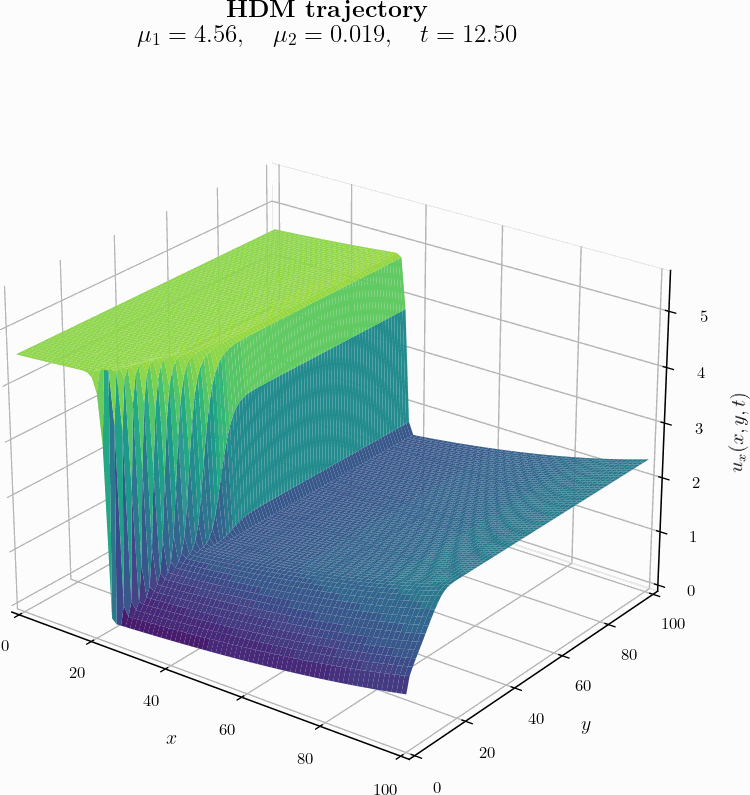
\includegraphics[height=0.56\textheight,keepaspectratio]{Figures/burgers_hdm_3d_transition_cropped.png}\\[0.20cm]
\Large Global and local HPROM validation\\[0.12cm]
\normalsize Linear POD bases, quadratic manifolds, and GPR manifolds
\end{frame}

\begin{frame}{Parameter Domain and Test Points}
\centering
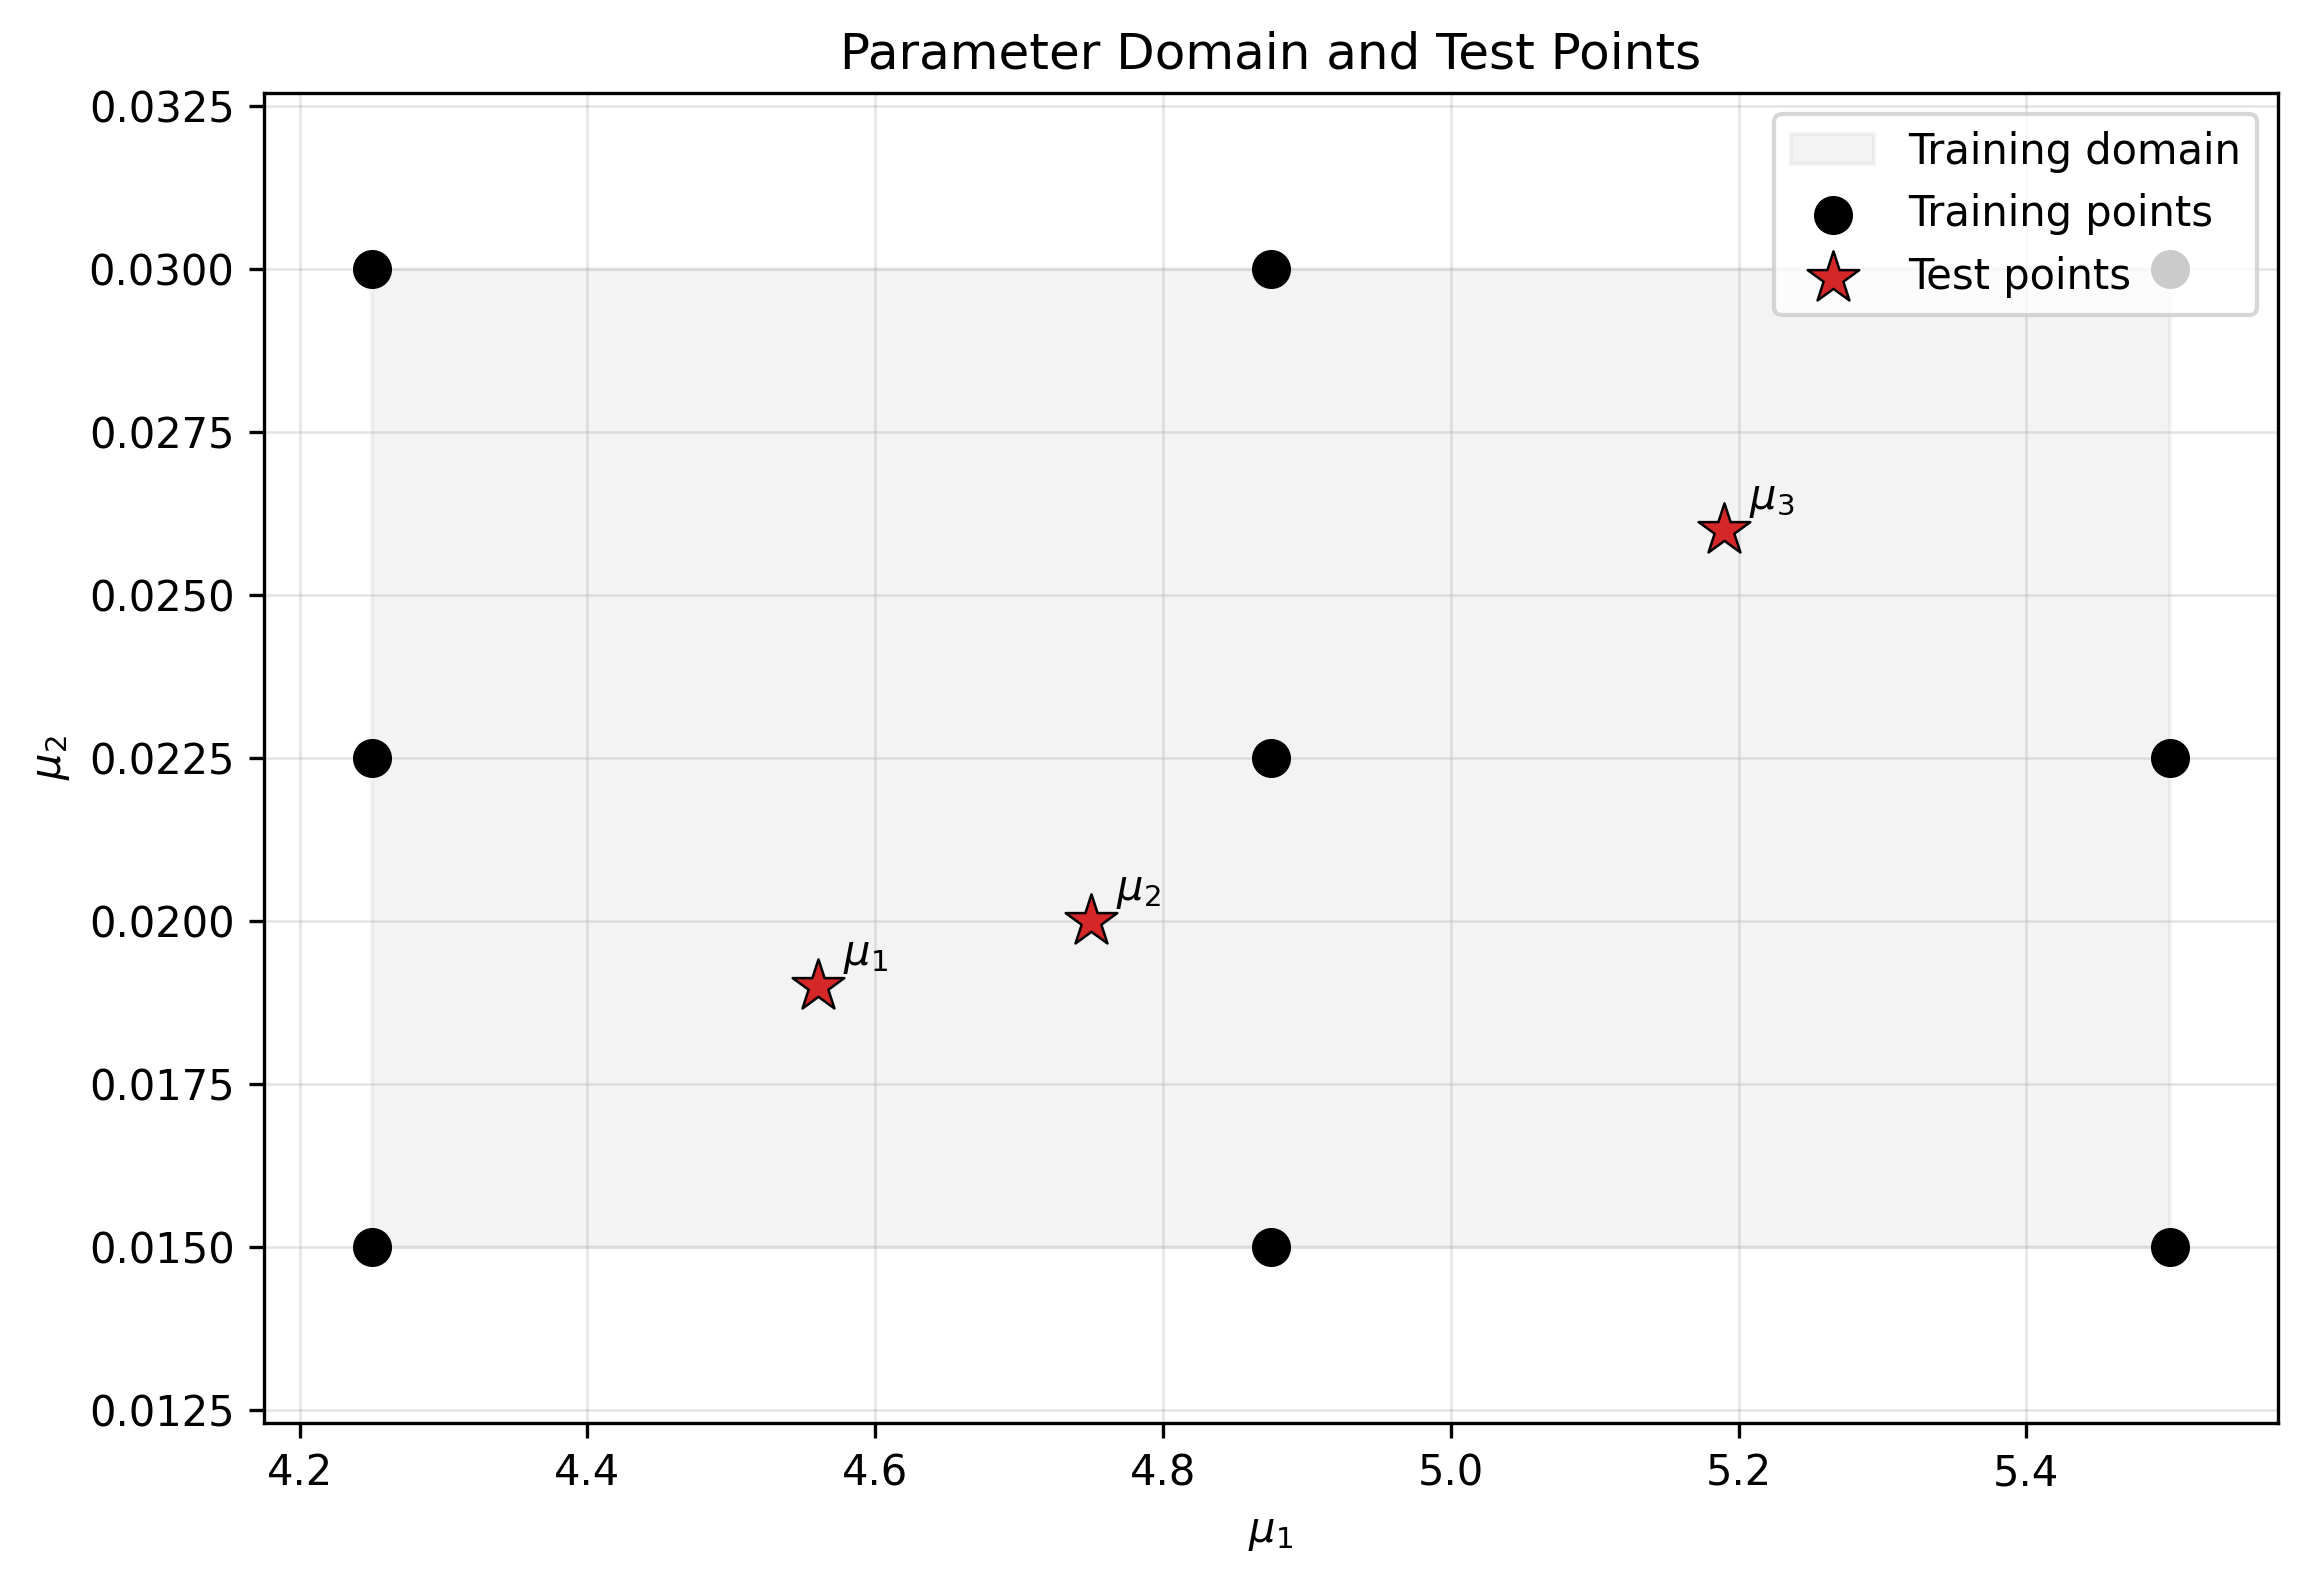
\includegraphics[width=0.82\textwidth,height=0.70\textheight,keepaspectratio]{Figures/parameter_domain_and_test_points.png}
\end{frame}

\newcommand{\BurgersTheoryFrames}{%
\begin{frame}{Global ROM Storyline: LSPG + Gauss-Newton}
\small
Given the implicit HDM residual $\mathbf{r}(\mathbf{u})=\mathbf{0}$, define a manifold
\[
\mathbf{u}\approx \mathbf{u}_{\mathrm{ref}}+\widetilde{\mathbf{u}}(\mathbf{q}).
\]
LSPG solves at each time step:
\[
\mathbf{q}^{\star}
=\arg\min_{\mathbf{q}}\;
\frac{1}{2}\left\|\mathbf{r}\!\left(\mathbf{u}_{\mathrm{ref}}+\widetilde{\mathbf{u}}(\mathbf{q})\right)\right\|_2^2.
\]
With Gauss-Newton (current iterate $\mathbf{q}^{(k)}$), the increment $\Delta\mathbf{q}$ is obtained from
\[
\left(\mathbf{\Psi}^{T}\mathbf{J}^{T}\mathbf{J}\mathbf{\Psi}\right)\Delta\mathbf{q}
=-\mathbf{\Psi}^{T}\mathbf{J}^{T}\mathbf{r},
\]
where
\[
\mathbf{\Psi}=\frac{\partial\widetilde{\mathbf{u}}}{\partial\mathbf{q}},
\qquad
\mathbf{J}=\frac{\partial\mathbf{r}}{\partial\mathbf{u}},
\qquad
\mathbf{q}^{(k+1)}=\mathbf{q}^{(k)}+\Delta\mathbf{q}.
\]
\end{frame}

\begin{frame}{Global Linear HPROM}
\small
State ansatz:
\[
\mathbf{u}\approx \mathbf{u}_{\mathrm{ref}}+\mathbf{V}\mathbf{q},
\qquad
\mathbf{V}\in\mathbb{R}^{N\times n},\; n=96.
\]
Hence
\[
\widetilde{\mathbf{u}}(\mathbf{q})=\mathbf{V}\mathbf{q},
\qquad
\mathbf{\Psi}=\frac{\partial\widetilde{\mathbf{u}}}{\partial\mathbf{q}}=\mathbf{V}.
\]
Gauss-Newton system:
\[
\left(\mathbf{V}^{T}\mathbf{J}^{T}\mathbf{J}\mathbf{V}\right)\Delta\mathbf{q}
=-\mathbf{V}^{T}\mathbf{J}^{T}\mathbf{r}.
\]
\end{frame}

\begin{frame}{Global HQPROM}
\small
Quadratic-manifold ansatz:
\[
\mathbf{u}\approx
\mathbf{u}_{\mathrm{ref}}
+\mathbf{V}\mathbf{q}
+\mathbf{H}\left(\mathbf{q}\otimes\mathbf{q}\right),
\qquad
n=39.
\]
Thus
\[
\widetilde{\mathbf{u}}(\mathbf{q})
=\mathbf{V}\mathbf{q}
+\mathbf{H}\left(\mathbf{q}\otimes\mathbf{q}\right),
\]
and the tangent depends on the current reduced state:
\[
\mathbf{\Psi}(\mathbf{q})
=\frac{\partial\widetilde{\mathbf{u}}}{\partial\mathbf{q}}
=\mathbf{V}
+\frac{\partial}{\partial\mathbf{q}}
\!\left[\mathbf{H}\left(\mathbf{q}\otimes\mathbf{q}\right)\right].
\]
\end{frame}

\begin{frame}{Global HPROM-GPR}
\small
Split basis and reduced coordinates:
\[
\mathbf{V}_{\mathrm{tot}}=[\mathbf{V},\bar{\mathbf{V}}],
\qquad
\mathbf{q}_{\mathrm{tot}}=
\begin{bmatrix}
\mathbf{q}\\
\bar{\mathbf{q}}
\end{bmatrix}.
\]
\[
\bar{\mathbf{q}}=\mathcal{N}_{\mathrm{GPR}}(\mathbf{q}),
\qquad
n=20,\;\bar{n}=131.
\]
State ansatz:
\[
\mathbf{u}\approx
\mathbf{u}_{\mathrm{ref}}
+\widetilde{\mathbf{u}}(\mathbf{q}),
\]
\[
\widetilde{\mathbf{u}}(\mathbf{q})
=\mathbf{V}_{\mathrm{tot}}\mathbf{q}_{\mathrm{tot}}
=\mathbf{V}\mathbf{q}
+\bar{\mathbf{V}}\,\mathcal{N}_{\mathrm{GPR}}(\mathbf{q}).
\]
Effective tangent for Gauss-Newton:
\[
\mathbf{\Psi}(\mathbf{q})
=\frac{\partial\widetilde{\mathbf{u}}}{\partial\mathbf{q}}
=\mathbf{V}
+\bar{\mathbf{V}}\frac{\partial\mathcal{N}_{\mathrm{GPR}}}{\partial\mathbf{q}}.
\]
\end{frame}

\begin{frame}{Local ROMs: Piecewise Manifolds}
\small
Partition the training snapshots into clusters $k=1,\dots,N_c$ and build one local trial manifold per cluster:
\[
\mathbf u \approx \Phi_k(\mathbf q_k).
\]

Examples used in this work:
\[
\Phi_k^{\mathrm{lin}}(\mathbf q)
=
\mathbf u_{0,k}+\mathbf V_k\mathbf q,
\]
\[
\Phi_k^{\mathrm{quad}}(\mathbf q)
=
\mathbf u_{0,k}+\mathbf V_k\mathbf q+\mathbf H_k(\mathbf q\otimes\mathbf q),
\]
\[
\Phi_k^{\mathrm{gpr}}(\mathbf q)
=
\mathbf u_{0,k}+\mathbf V_k\mathbf q+\bar{\mathbf V}_k\,\mathcal N_{\mathrm{GPR},k}(\mathbf q).
\]

\vspace{0.3em}
\textbf{Online workflow}
\begin{enumerate}
\item Select the active cluster.
\item If the cluster changes, transfer the current state to the new local manifold.
\item Solve the local LSPG problem in the active manifold.
\end{enumerate}
\end{frame}

\begin{frame}{Cluster Selection: Final Form (Linear)}
\small
Shared nearest-centroid selector (used in all local models):
\[
k^+=\arg\min_{\ell=1,\dots,N_c}\|\mathbf u^s-\mathbf u_{c,\ell}\|_2^2,
\qquad
\mathbf u^s=\Phi_{k^-}(\mathbf q_{k^-}).
\]

\vspace{0.2em}
For the linear local manifold $\Phi_{k^-}^{\mathrm{lin}}(\mathbf q)=\mathbf u_{0,k^-}+\mathbf V_{k^-}\mathbf q$:
\[
k^+=\arg\min_{\ell=1,\dots,N_c} S_{k^-,\ell}^{\mathrm{lin}}(\mathbf q_{k^-}),
\]
\[
S_{k^-,\ell}^{\mathrm{lin}}(\mathbf q)
=
2\,\mathbf g_{k^-,\ell}^T\mathbf q + d_{k^-,\ell},
\]
with offline-precomputed terms
\[
\mathbf g_{k^-,\ell}
:=
\mathbf V_{k^-}^T(\mathbf u_{0,k^-}-\mathbf u_{c,\ell}),
\qquad
d_{k^-,\ell}
:=
\|\mathbf u_{0,k^-}-\mathbf u_{c,\ell}\|_2^2.
\]
\end{frame}

\begin{frame}{Cluster Selection: Final Form (HQPROM and HPROM-GPR)}
\scriptsize
\textbf{HQPROM selector}
\[
k^+=\arg\min_{\ell} S_{k^-,\ell}^{\mathrm{quad}}(\mathbf q_{k^-}),
\]
\[
S_{k^-,\ell}^{\mathrm{quad}}(\mathbf q)
=
2\,\mathbf g_{k^-,\ell}^T\mathbf q
+
2\,\mathbf m_{k^-,\ell}^T(\mathbf q\otimes\mathbf q)
+
d_{k^-,\ell},
\]
\[
\mathbf m_{k^-,\ell}^T(\mathbf q\otimes\mathbf q)
:=
(\mathbf u_{0,k^-}-\mathbf u_{c,\ell})^T\mathbf H_{k^-}(\mathbf q\otimes\mathbf q).
\]

\vspace{0.35em}
\textbf{HPROM-GPR selector}
\[
k^+=\arg\min_{\ell} S_{k^-,\ell}^{\mathrm{gpr}}(\mathbf q_{k^-}),
\]
\[
S_{k^-,\ell}^{\mathrm{gpr}}(\mathbf q)
=
2\,\mathbf g_{k^-,\ell}^T\mathbf q
+
2\,\bar{\mathbf g}_{k^-,\ell}^T\mathcal N_{\mathrm{GPR},k^-}(\mathbf q)
+
d_{k^-,\ell}.
\]
\[
\bar{\mathbf q}_{k^-}:=\mathcal N_{\mathrm{GPR},k^-}(\mathbf q_{k^-}),
\qquad
\bar{\mathbf g}_{k^-,\ell}:=\bar{\mathbf V}_{k^-}^T(\mathbf u_{0,k^-}-\mathbf u_{c,\ell}).
\]
\end{frame}

\begin{frame}{Cluster Change: Linear and Nonlinear Transfers}
\scriptsize
\[
k^+=k^- \Rightarrow \text{no transfer},
\qquad
k^+\neq k^- \Rightarrow \text{solve transfer problem}.
\]
Transferred state:
\[
\mathbf u^s=\Phi_{k^-}(\mathbf q_{k^-}).
\]

\textbf{Linear local target}
\[
\mathbf q_{k^+}^{\mathrm{lin}}
=\arg\min_{\mathbf q}
\left\|
\mathbf u^s-\left(\mathbf u_{0,k^+}+\mathbf V_{k^+}\mathbf q\right)
\right\|_2^2,
\]
\[
\text{if }\mathbf V_{k^+}^T\mathbf V_{k^+}=\mathbf I,\quad
\mathbf q_{k^+}^{\mathrm{lin}}=\mathbf V_{k^+}^T(\mathbf u^s-\mathbf u_{0,k^+}).
\]

\textbf{Nonlinear local targets (HQPROM / HPROM-GPR)}
\[
\mathbf q_{k^+}^{\mathrm{nl}}
=\arg\min_{\mathbf q}
\left\|\mathbf u^s-\Phi_{k^+}^{\mathrm{nl}}(\mathbf q)\right\|_2^2.
\]
\end{frame}

\begin{frame}{Cluster Change: Nonlinear Least Squares}
\small
For nonlinear local manifolds, define
\[
\mathbf r_{\mathrm{tr}}(\mathbf q):=\Phi_{k^+}(\mathbf q)-\mathbf u^s,
\qquad
\mathbf J_{\Phi}(\mathbf q):=\frac{\partial \Phi_{k^+}}{\partial \mathbf q}.
\]
Gauss--Newton at iterate $\mathbf q^{(j)}$:
\[
\left(\mathbf J_{\Phi}^T\mathbf J_{\Phi}\right)\Delta\mathbf q
=
-\mathbf J_{\Phi}^T\mathbf r_{\mathrm{tr}}(\mathbf q^{(j)}),
\qquad
\mathbf q^{(j+1)}=\mathbf q^{(j)}+\Delta\mathbf q.
\]
\end{frame}

}

\begin{frame}{Online Performance ($250\times250$): Avg/Max Error over 3 Test Points}
\scriptsize
\centering
\resizebox{\textwidth}{!}{%
\begin{tabular}{lrrrrrrr}
\hline
\textbf{Computational model} & $n$ ($N$ for HDM) & $\bar{n}$ & $N_e$ & avg $\mathbb{RE}_{2,\mathbf{u}}$ (\%) & max $\mathbb{RE}_{2,\mathbf{u}}$ (\%) & Wall-clock time (min) & Speedup \\
\hline
HDM & 125\,000 & -- & 62\,500 & -- & -- & 12.517 & -- \\
\addlinespace[0.35em]
HPROM & 96 & -- & 4\,241 & 1.030 & 1.096 & 0.366 & 34.2 \\
HQPROM & 39 & -- & 3\,460 & 0.818 & 0.861 & 0.641 & 19.5 \\
HPROM-GPR & 20 & 131 & 1\,799 & 0.666 & 0.785 & 0.236 & 53.1 \\
\addlinespace[0.35em]
Local HPROM ($N_c=3$) & 35--48 & -- & 3\,405 & 0.897 & 0.933 & 0.154 & 81.4 \\
Local HQPROM ($N_c=3$) & 21--27 & -- & 2\,152 & 0.888 & 1.025 & 0.215 & 58.3 \\
Local HPROM-GPR ($N_c=3$) & 9 & 60--97 & 811 & 0.714 & 0.786 & 0.113 & 110.5 \\
\addlinespace[0.35em]
Local HPROM ($N_c=5$) & 23--31 & -- & 2\,384 & 0.915 & 0.943 & 0.095 & 132.0 \\
Local HQPROM ($N_c=5$) & 15--20 & -- & 1\,593 & 0.760 & 0.878 & 0.128 & 97.9 \\
Local HPROM-GPR ($N_c=5$) & 7 & 41--68 & 631 & 0.673 & 0.880 & 0.094 & 133.2 \\
\hline
\end{tabular}}
\vspace{0.2em}

{\tiny Speedup is computed with respect to the HDM runtime, $t_{\mathrm{HDM}}=751.043$ s, averaged over the three test points.}

{\tiny Online timings were measured on Sherlock using one node, 24 MPI ranks, and 24 cores.}

{\tiny $N_e$ denotes the number of sampled ECSW elements ($N_e=62{,}500$ for HDM/full mesh).}

{\tiny All models are reported at a matched accuracy target of $1\% \pm 0.2\%$ in max $\mathbb{RE}_{2,\mathbf{u}}$: for each $N_c$ the accuracy knob is tuned into that window ($\mathtt{pod\_tol}$ for Local HPROM, $\zeta_{\mathrm{qua}}$ for Local HQPROM, $n$ for Local HPROM-GPR), so differences in $n$, $N_e$ and speedup are read at constant accuracy.}
\end{frame}

\begin{frame}{Global Reduced Meshes (ECSW)}
\centering
\begin{columns}[T]
\column{0.33\textwidth}
\centering
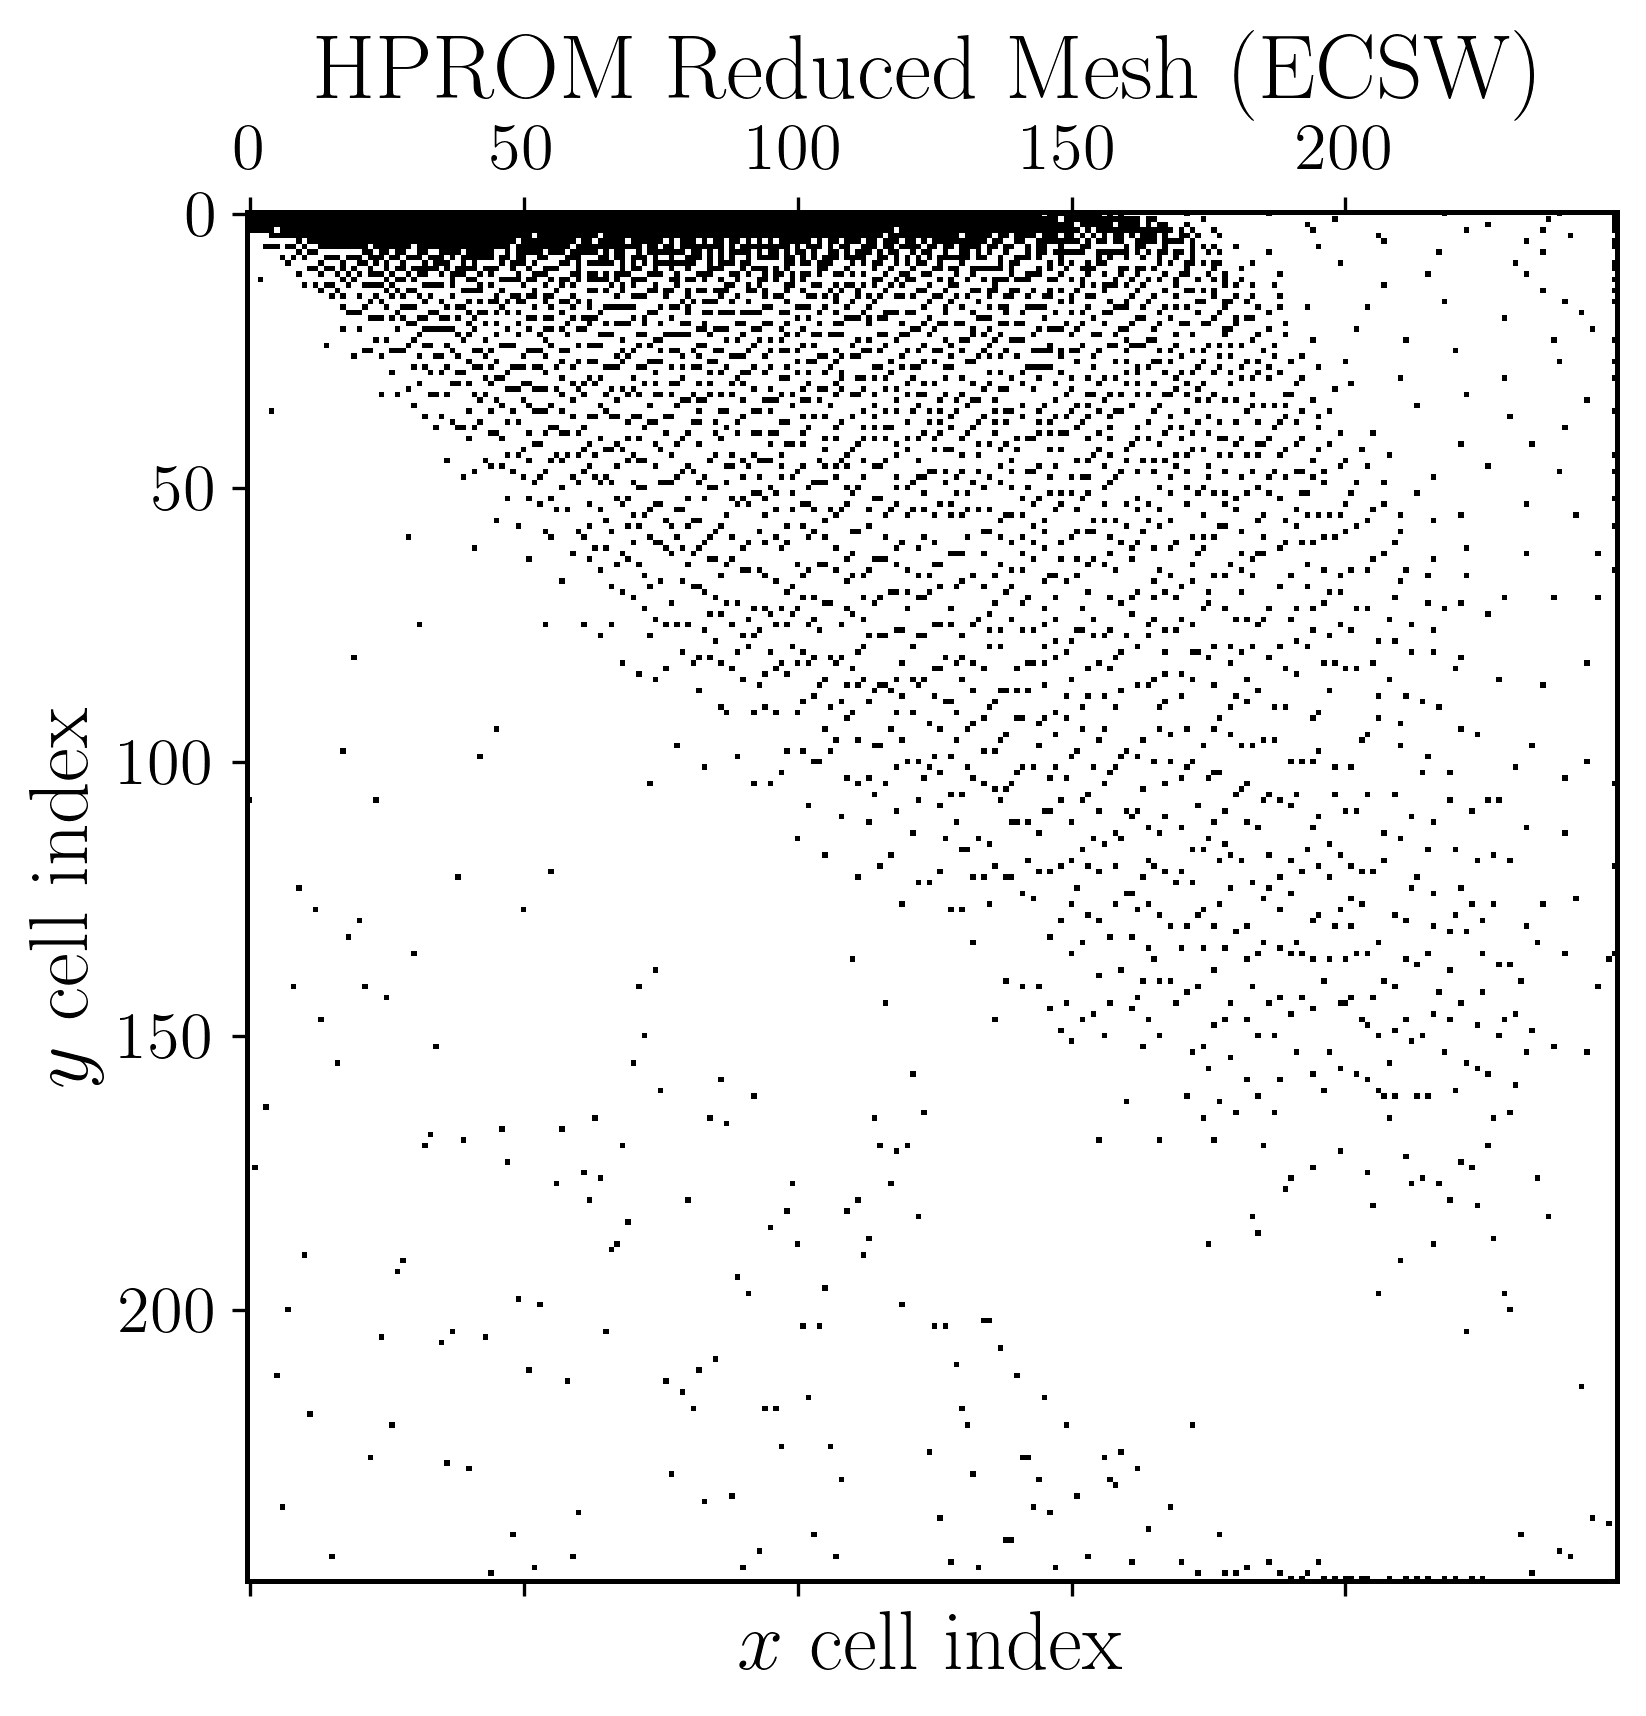
\includegraphics[width=\linewidth]{hprom_reduced_mesh.png}\\
{\tiny HPROM ($N_e=4{,}241$)}

\column{0.33\textwidth}
\centering
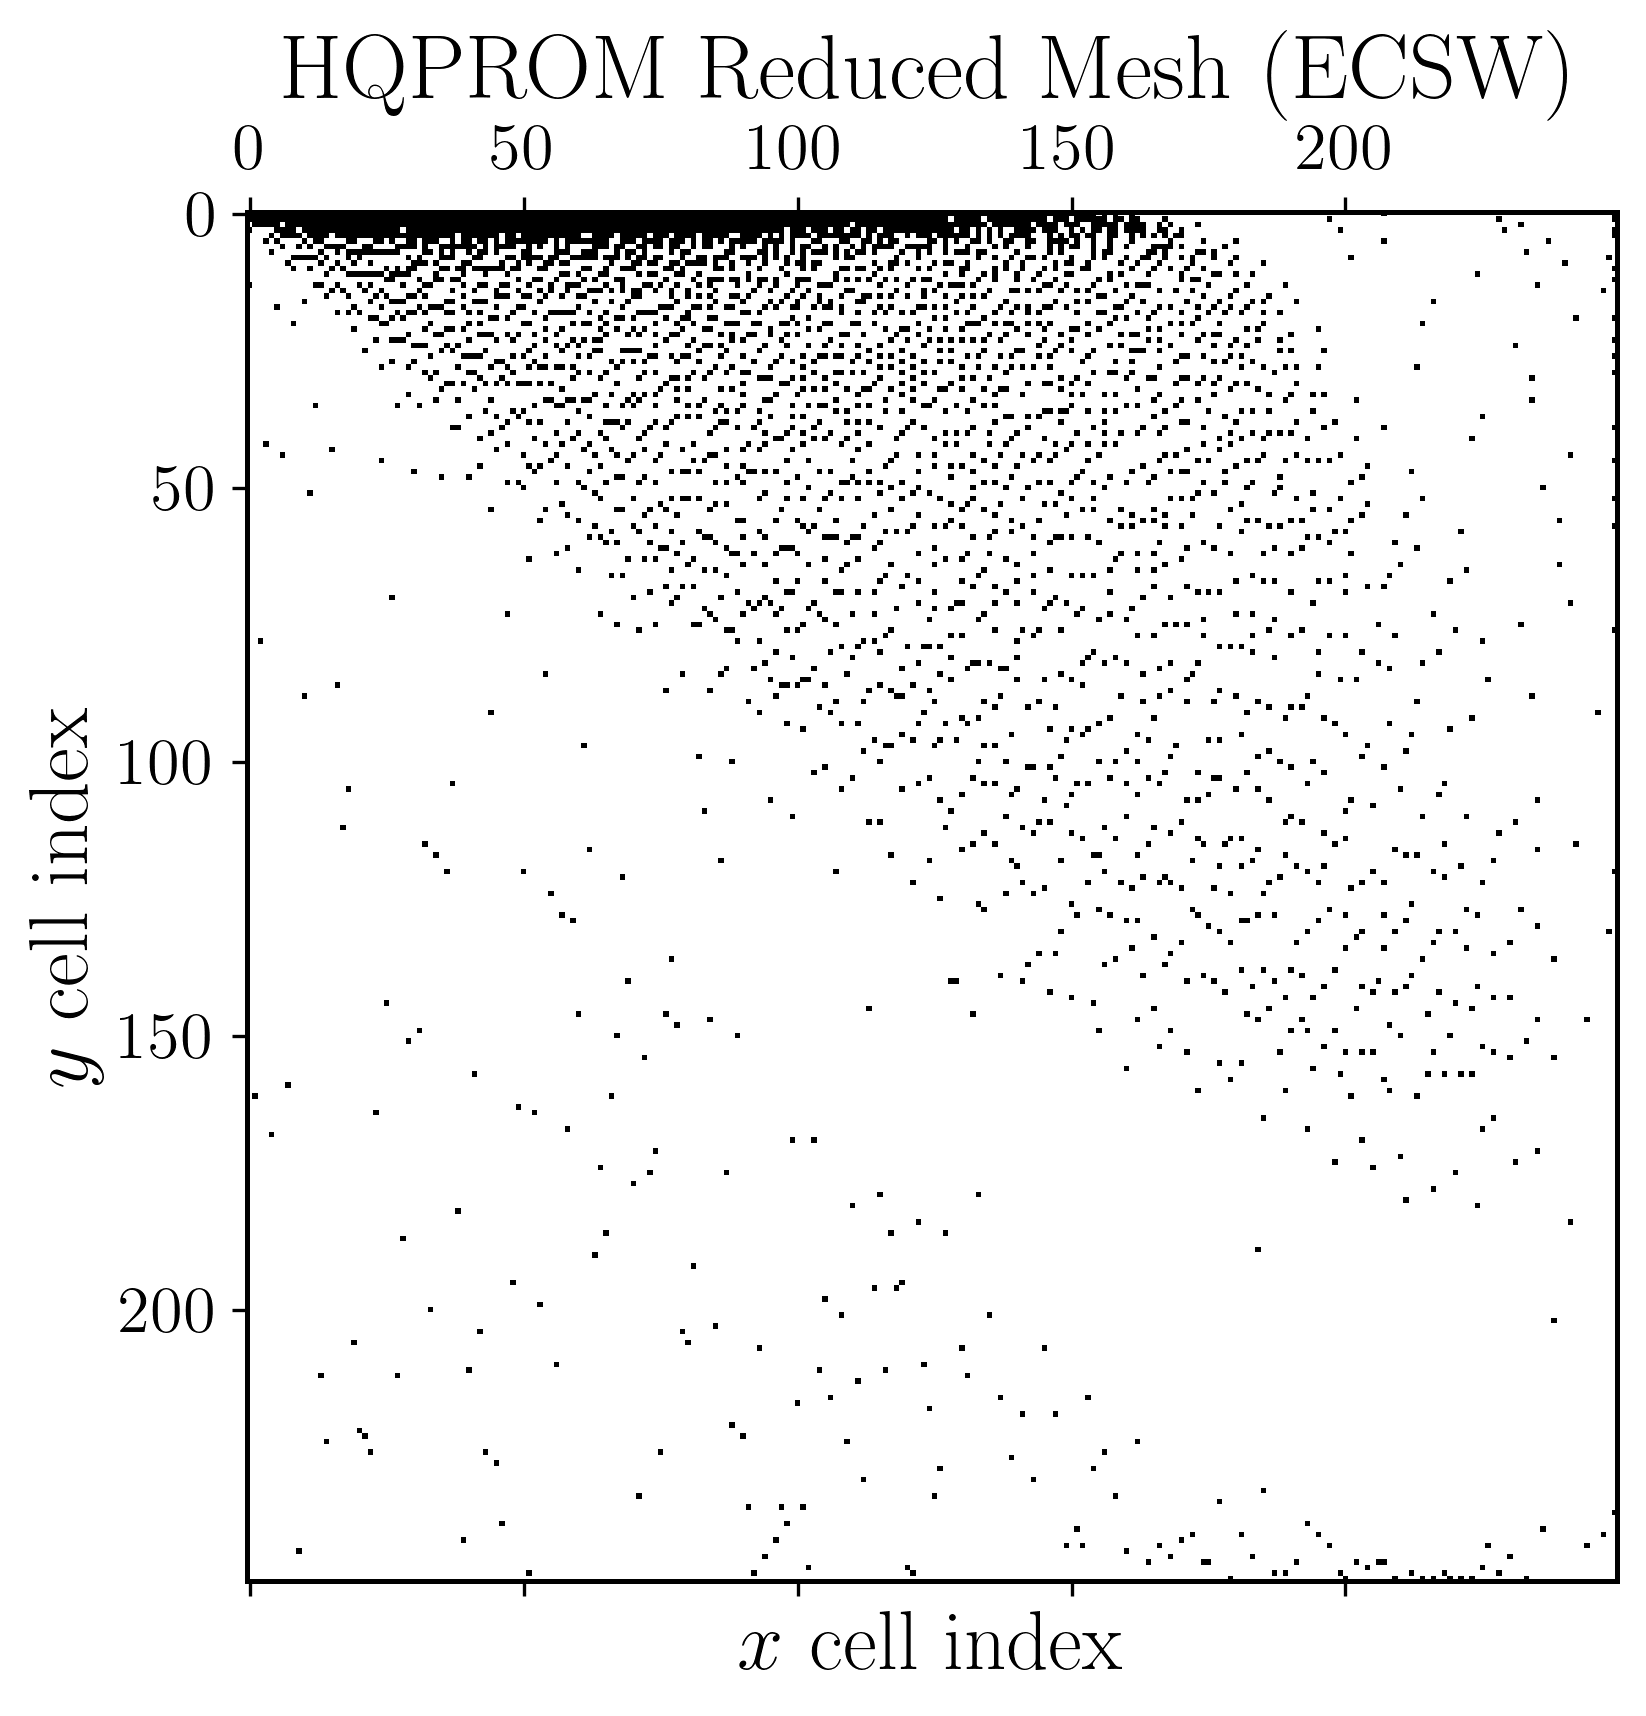
\includegraphics[width=\linewidth]{hqprom_reduced_mesh.png}\\
{\tiny HQPROM ($N_e=3{,}460$)}

\column{0.33\textwidth}
\centering
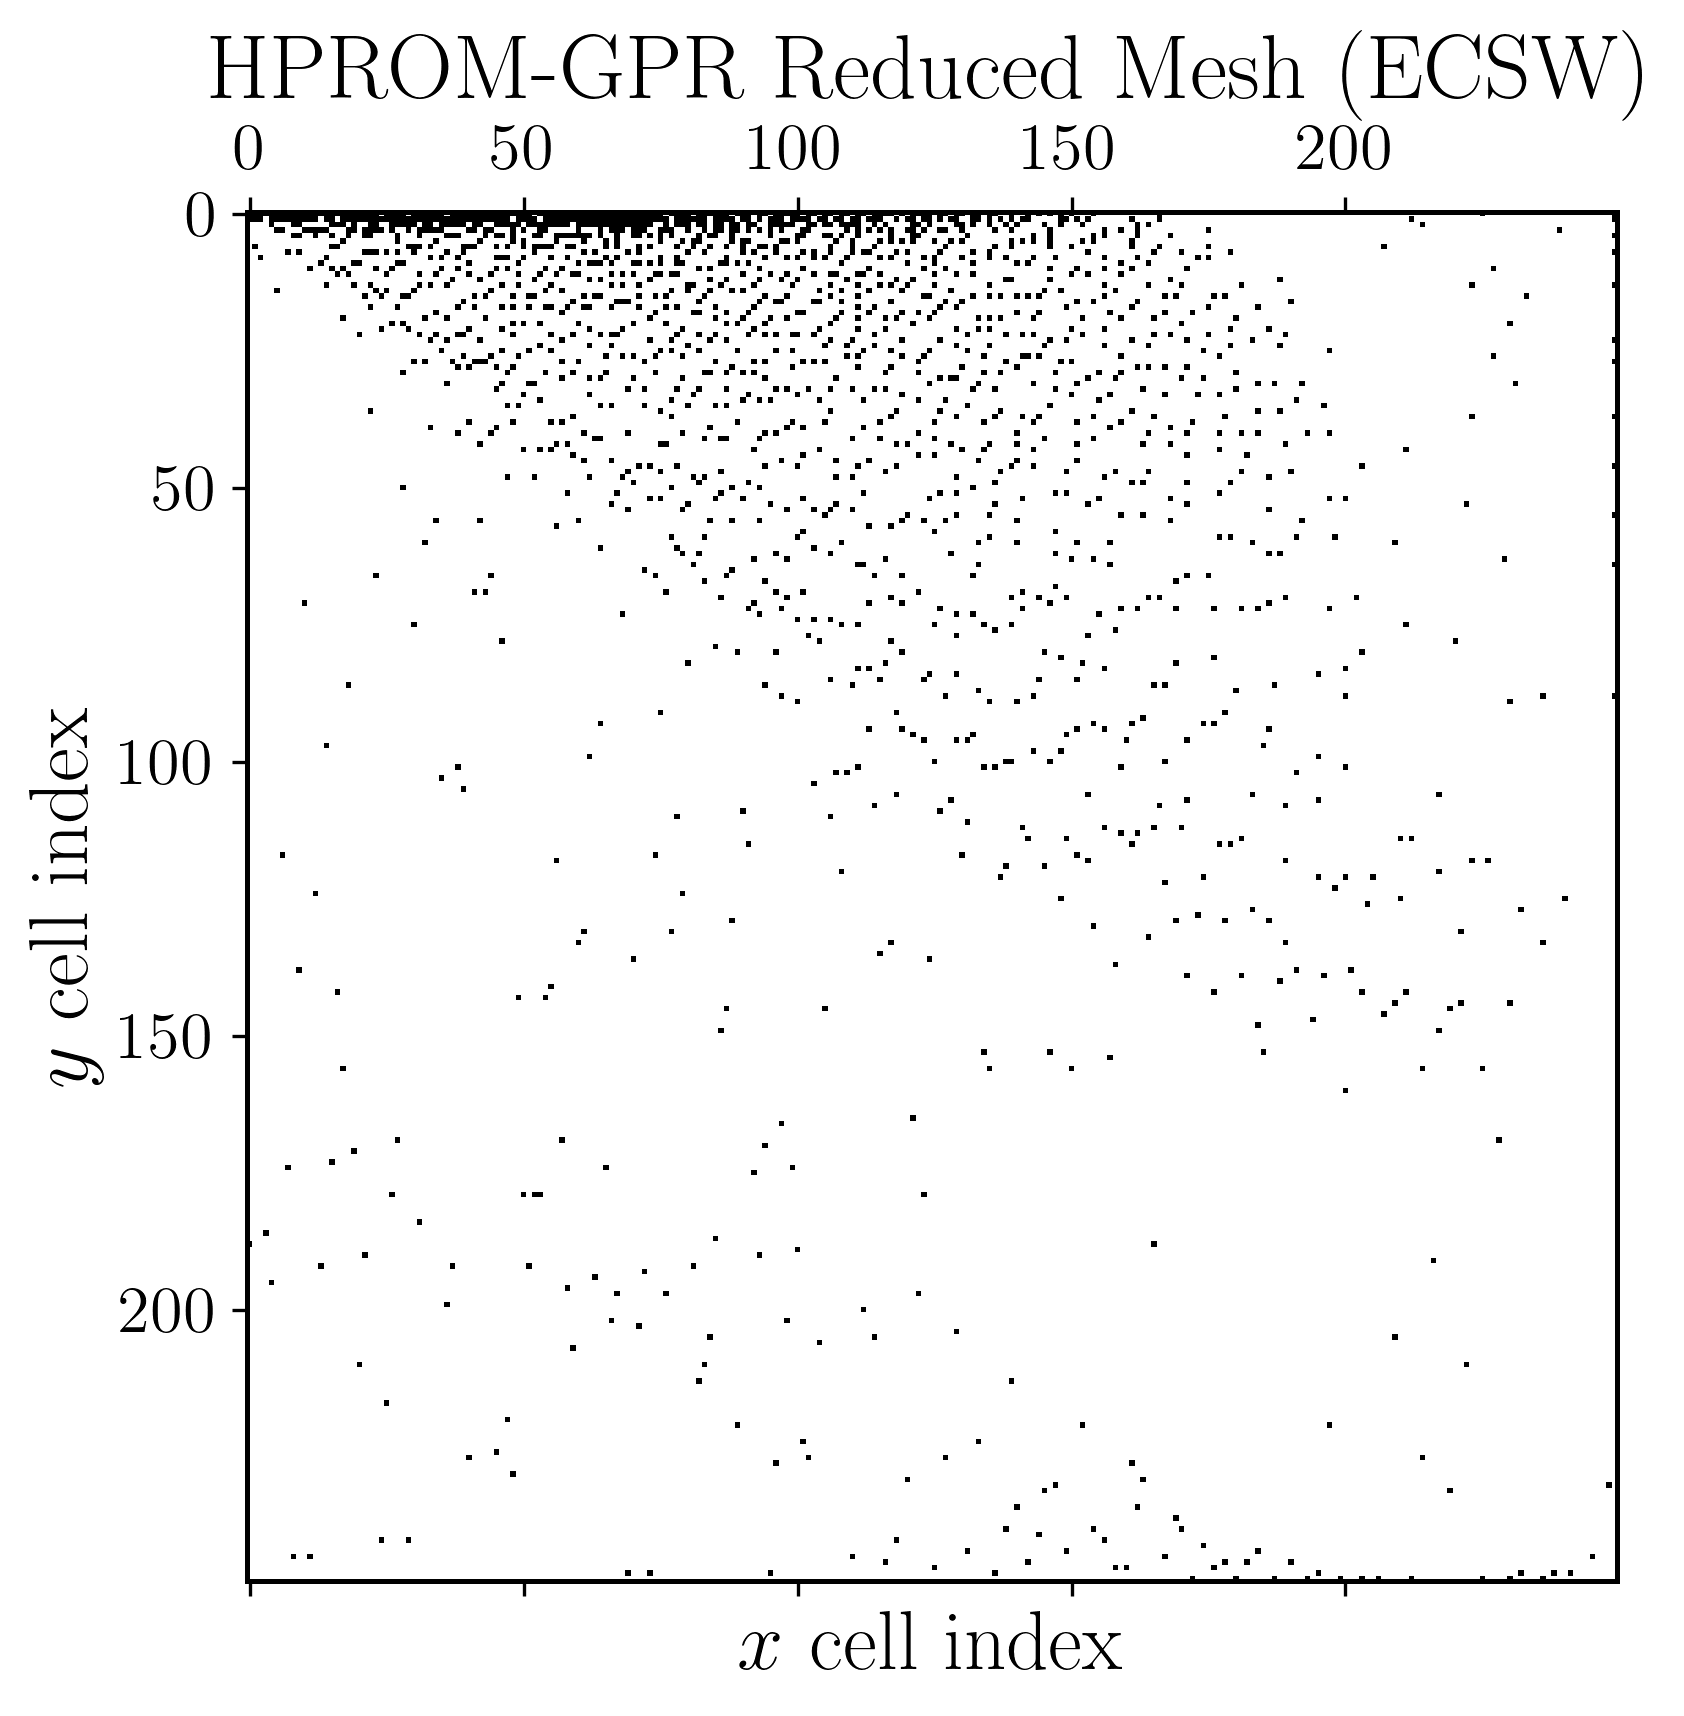
\includegraphics[width=\linewidth]{hprom_gpr_reduced_mesh.png}\\
{\tiny HPROM-GPR ($N_e=1{,}799$)}
\end{columns}
\end{frame}

\begin{frame}{Local Reduced Meshes (ECSW), $N_c=3$}
\centering
\begin{columns}[T]
\column{0.33\textwidth}
\centering
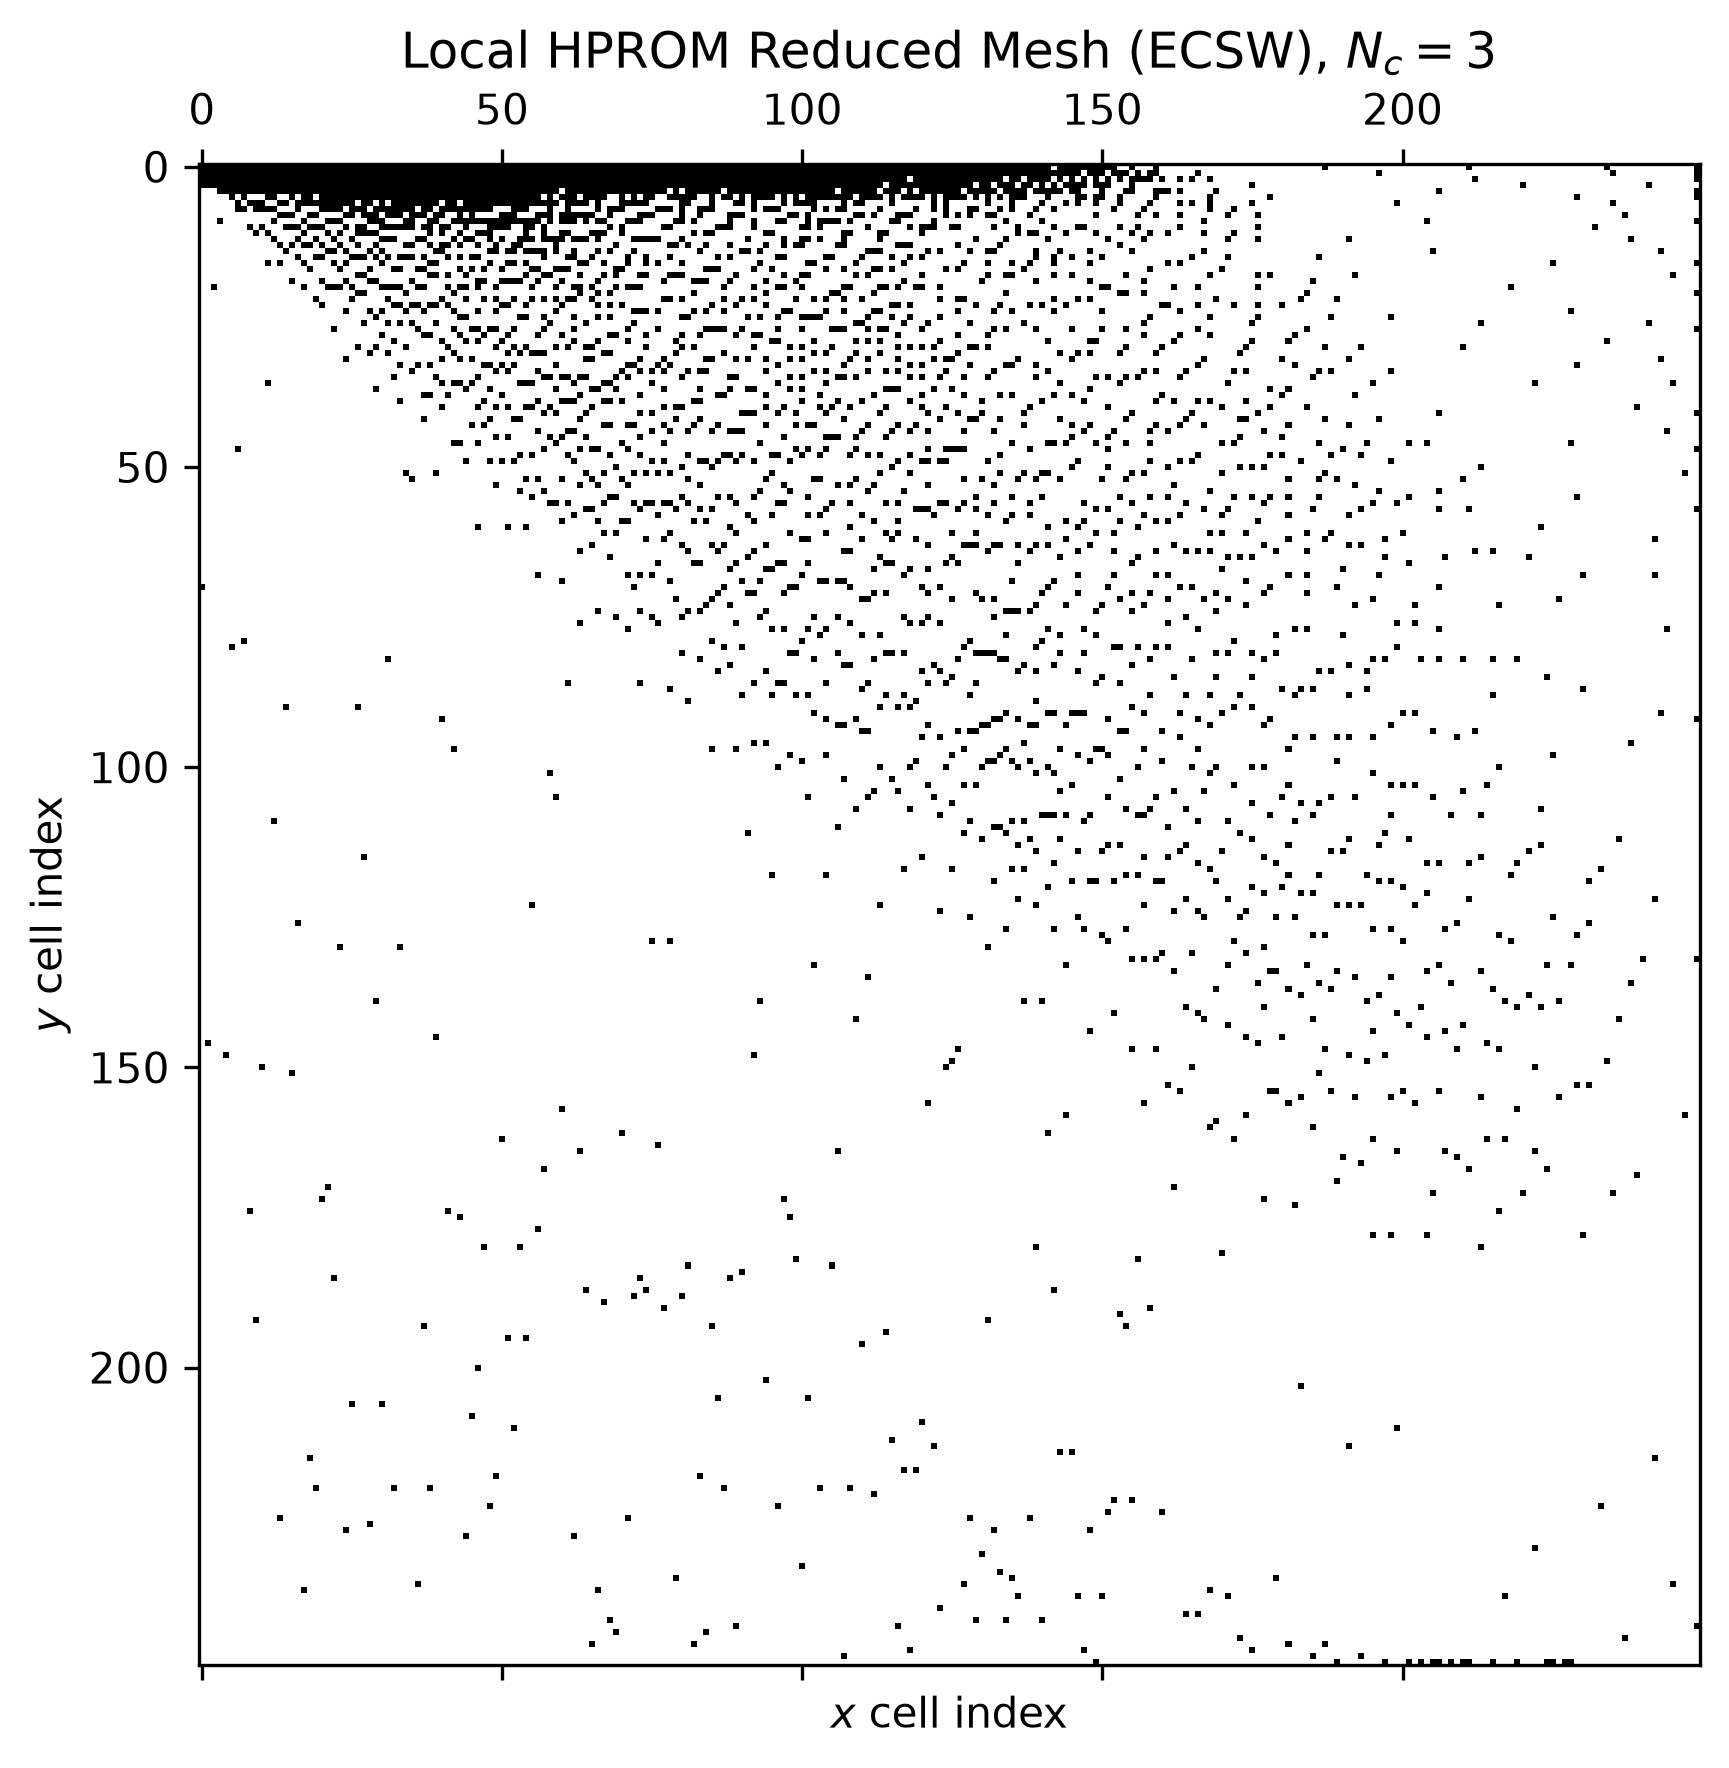
\includegraphics[width=\linewidth]{local_hprom_reduced_mesh.png}\\
{\tiny Local HPROM ($N_e=3{,}405$)}

\column{0.33\textwidth}
\centering
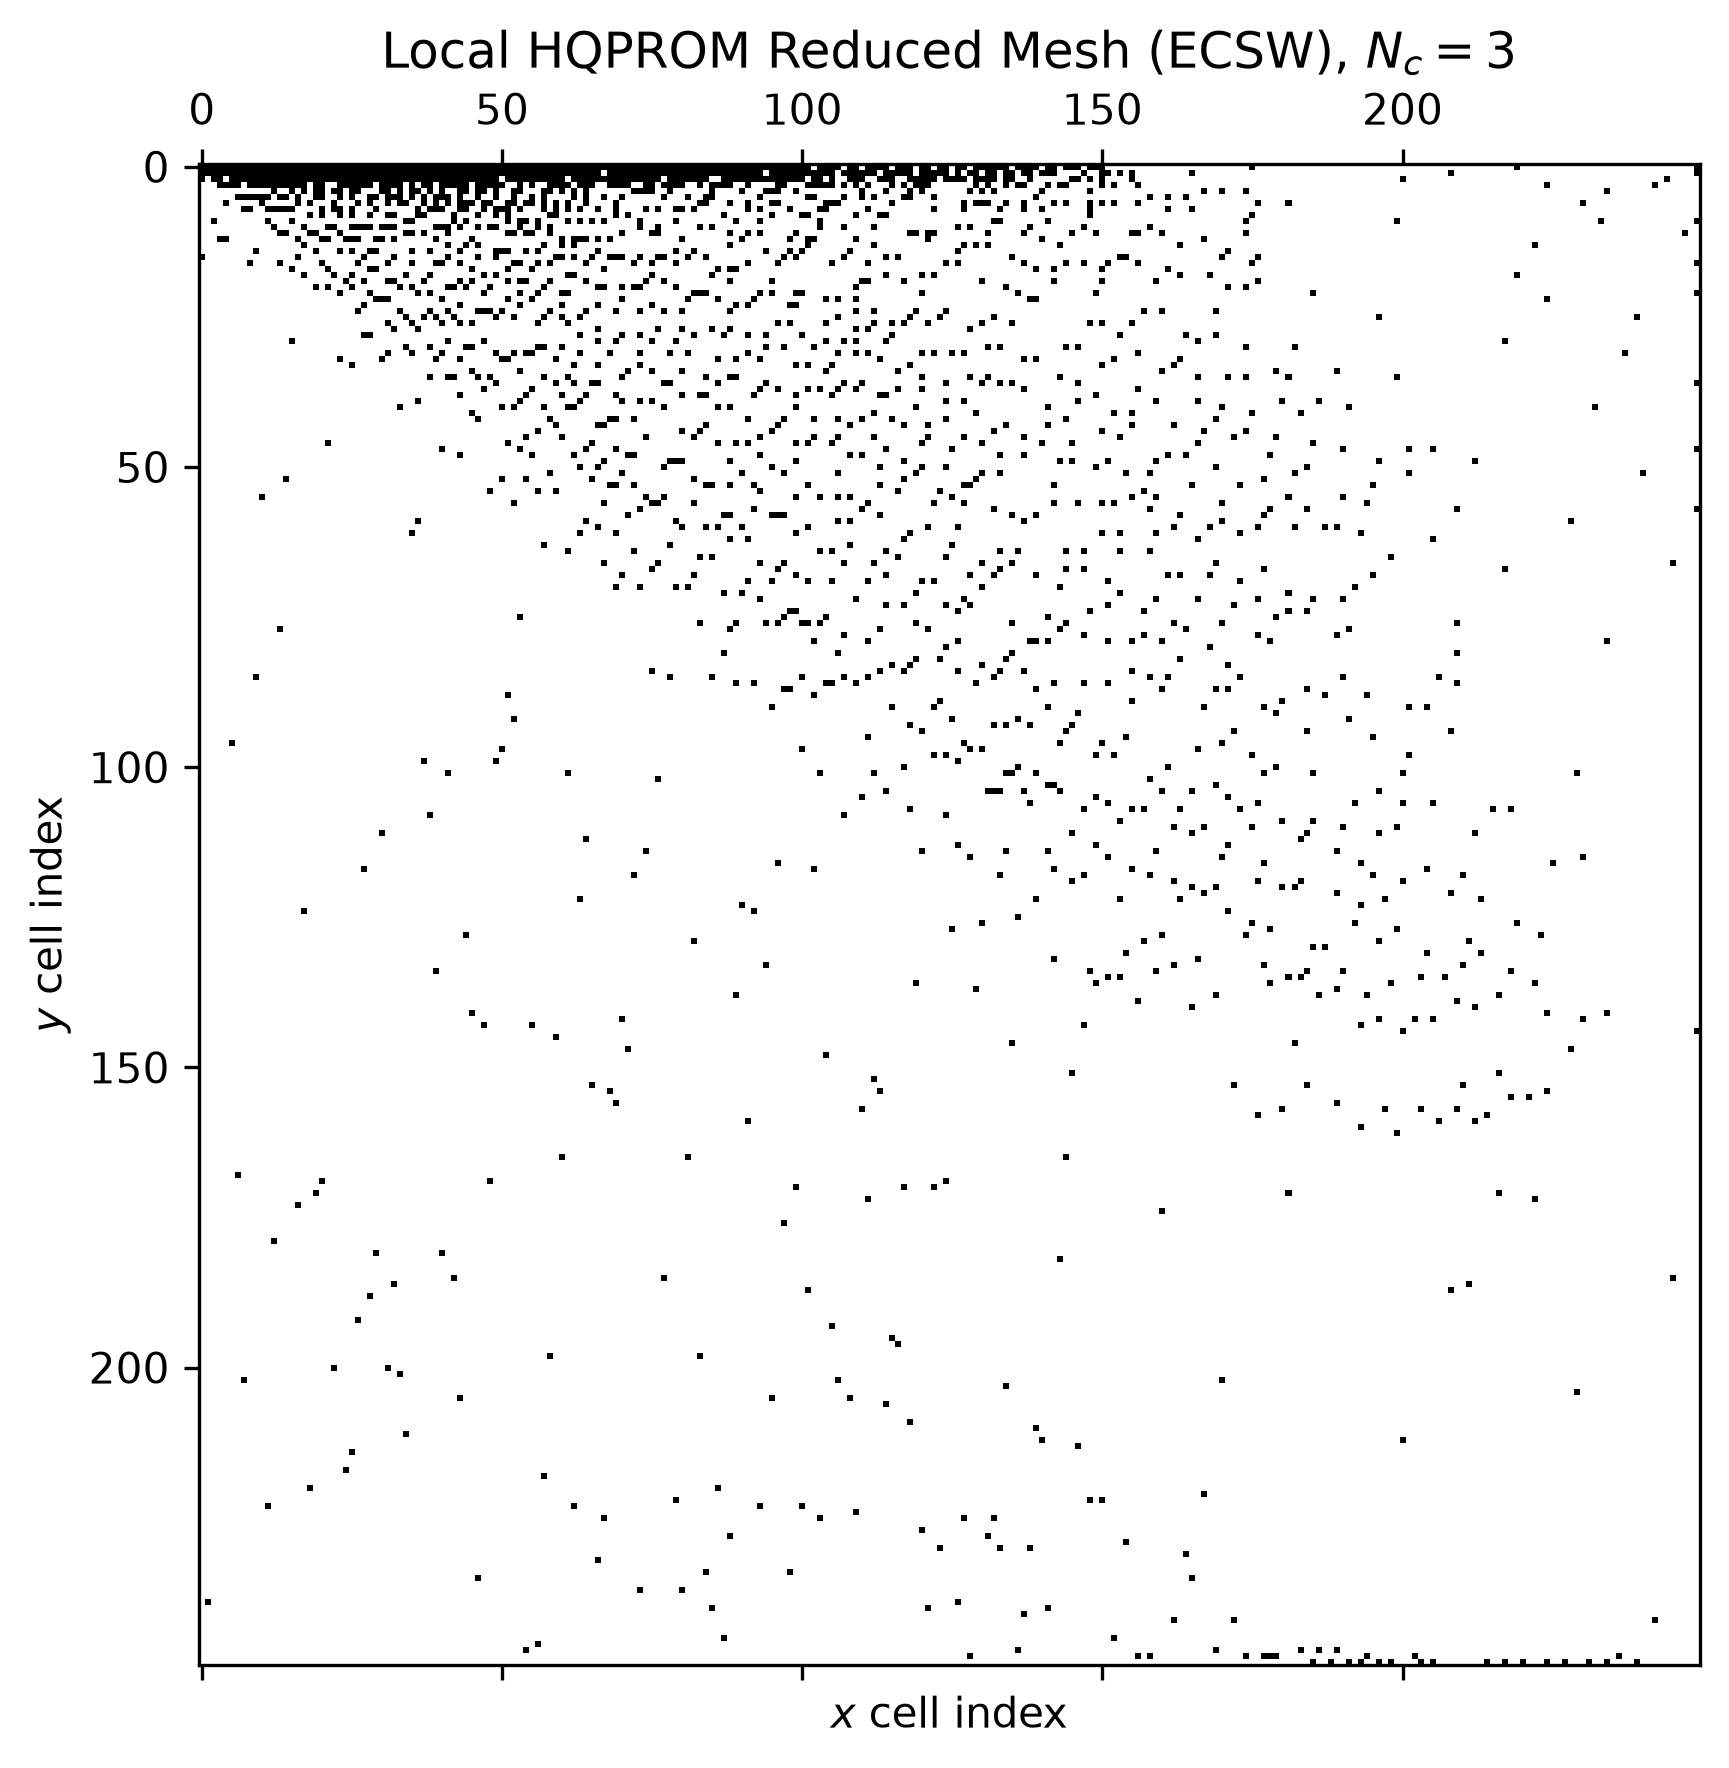
\includegraphics[width=\linewidth]{local_hqprom_reduced_mesh.png}\\
{\tiny Local HQPROM ($N_e=2{,}152$)}

\column{0.33\textwidth}
\centering
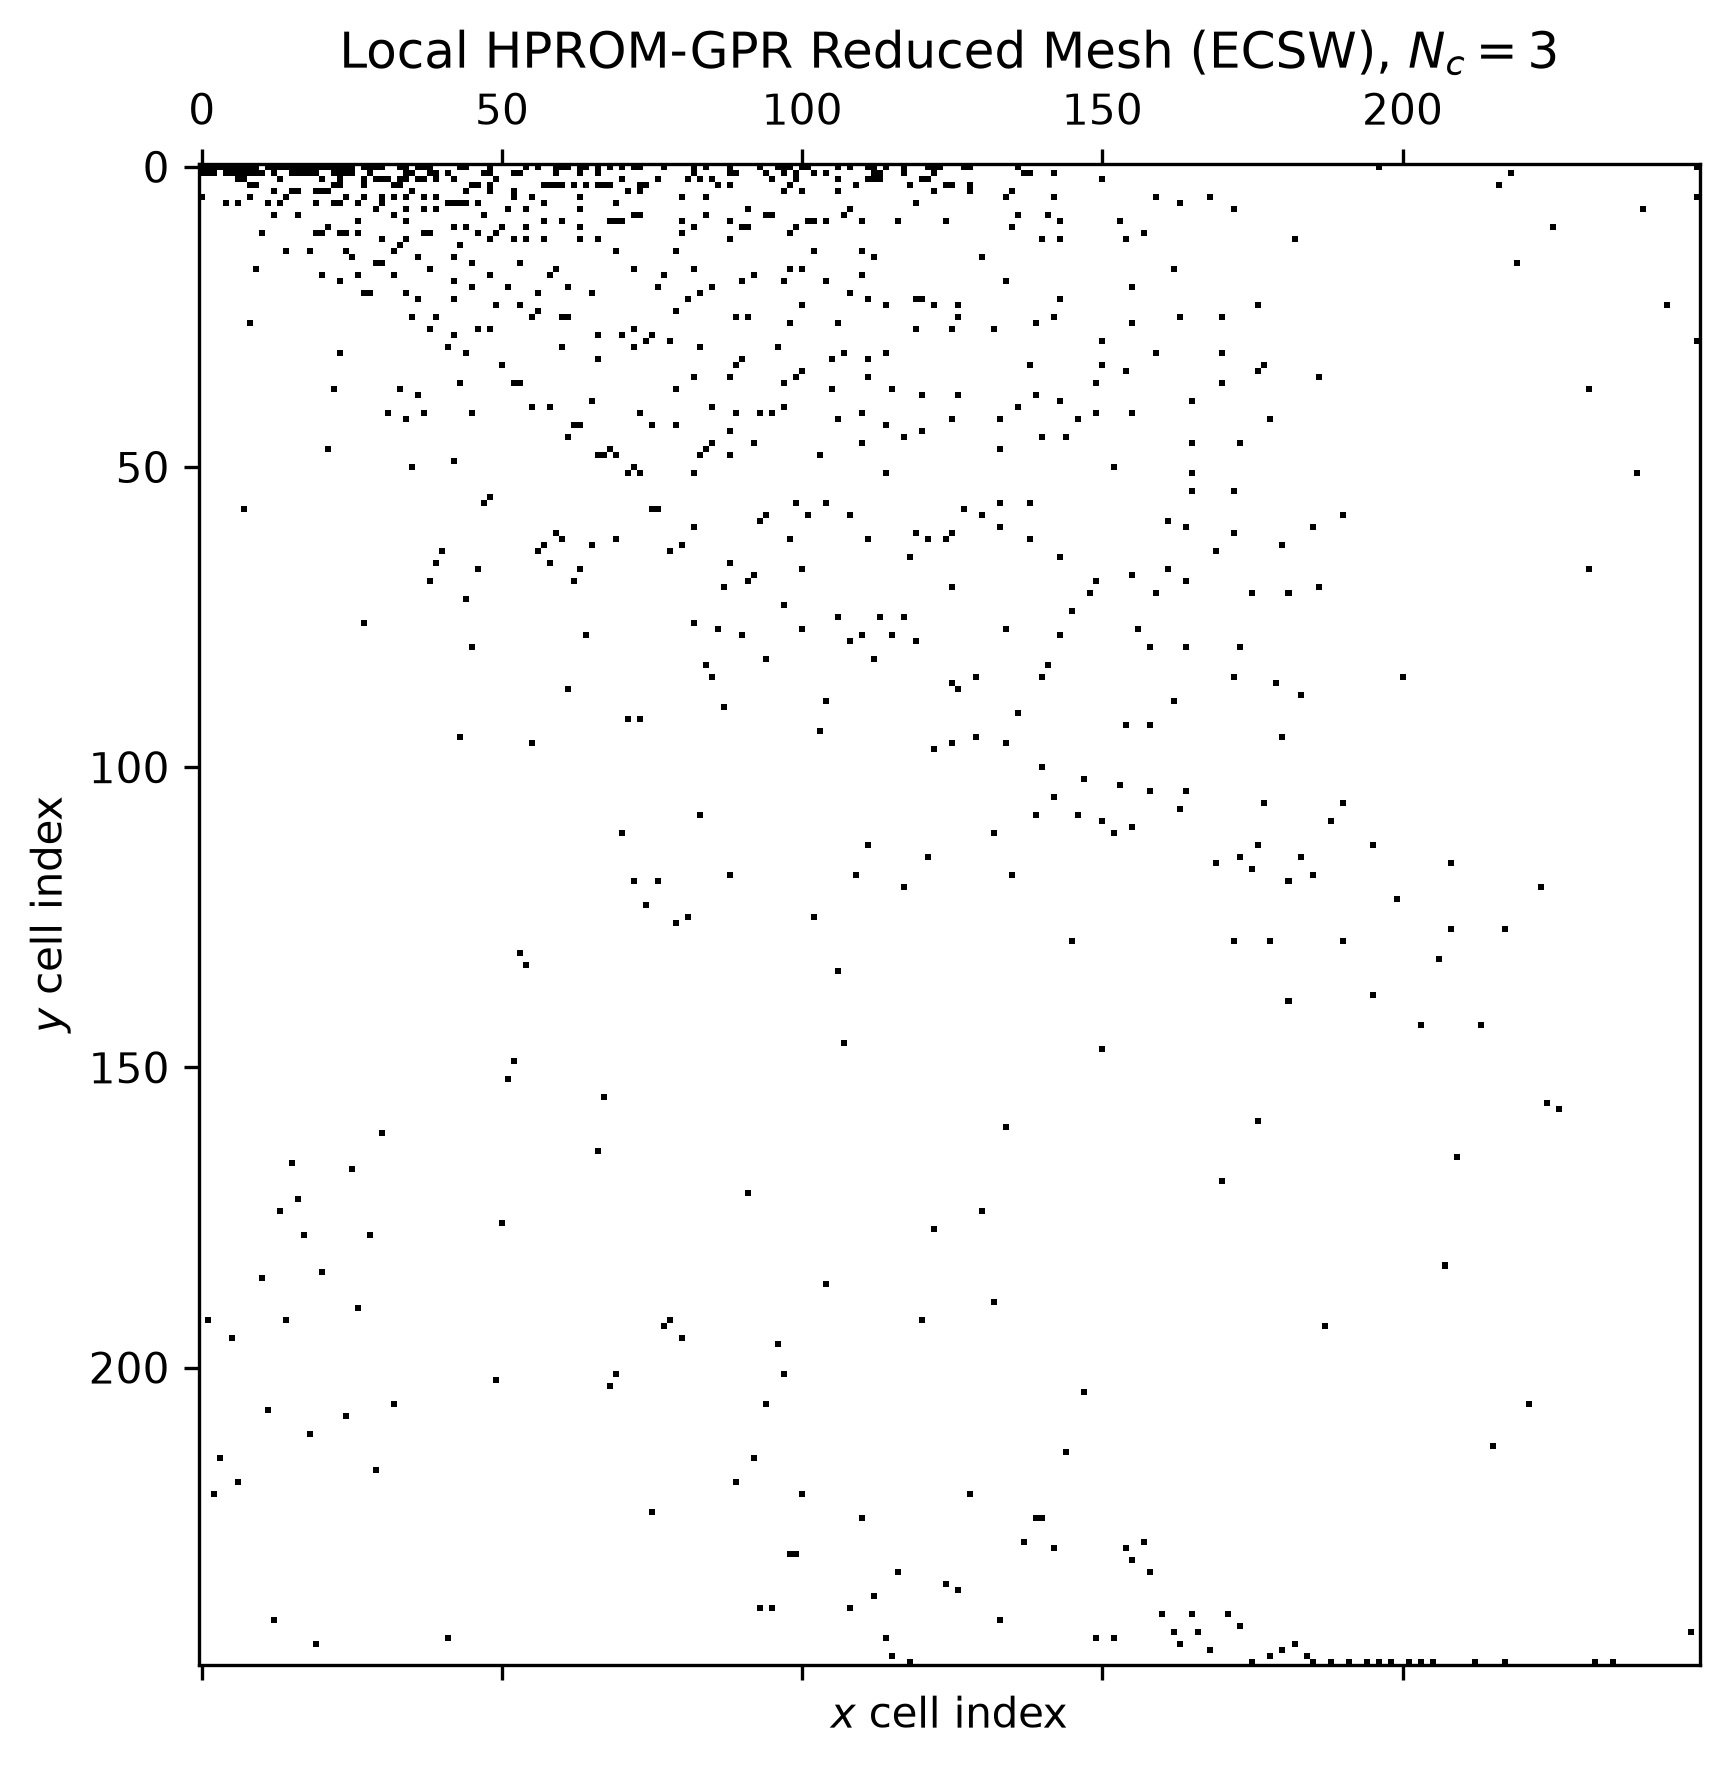
\includegraphics[width=\linewidth]{local_hprom_gpr_reduced_mesh.png}\\
{\tiny Local HPROM-GPR ($N_e=811$)}
\end{columns}
\end{frame}

\begin{frame}{Burgers Observations}
\small
\begin{itemize}
  \item Clustering accelerates all three families, monotonically from global to
        $N_c=3$ to $N_c=5$.
  \item The linear basis has the most to gain from it, since it starts without any
        compression of its own, and by $N_c=5$ it draws level with local GPR
        ($132\times$ versus $133\times$).
  \item The two mechanisms therefore overlap: clustering and nonlinear compression both
        reduce the local dimension, so their gains are not simply additive. How much each
        contributes appears to be problem dependent.
\end{itemize}

\vspace{0.3em}
{\footnotesize Timings come from a Python implementation and are indicative: the
nonlinear models carry the most per-step overhead, so they have the most to gain from
vectorization, and their speedups are lower bounds rather than limits of the method.
This shows up most in HQPROM against HPROM.}
\end{frame}

\newcommand{\BurgersSolutionFigureFrames}{%
\begin{frame}{HPROM vs HDM: $\boldsymbol\mu=(4.56,\,0.019)$}
\centering
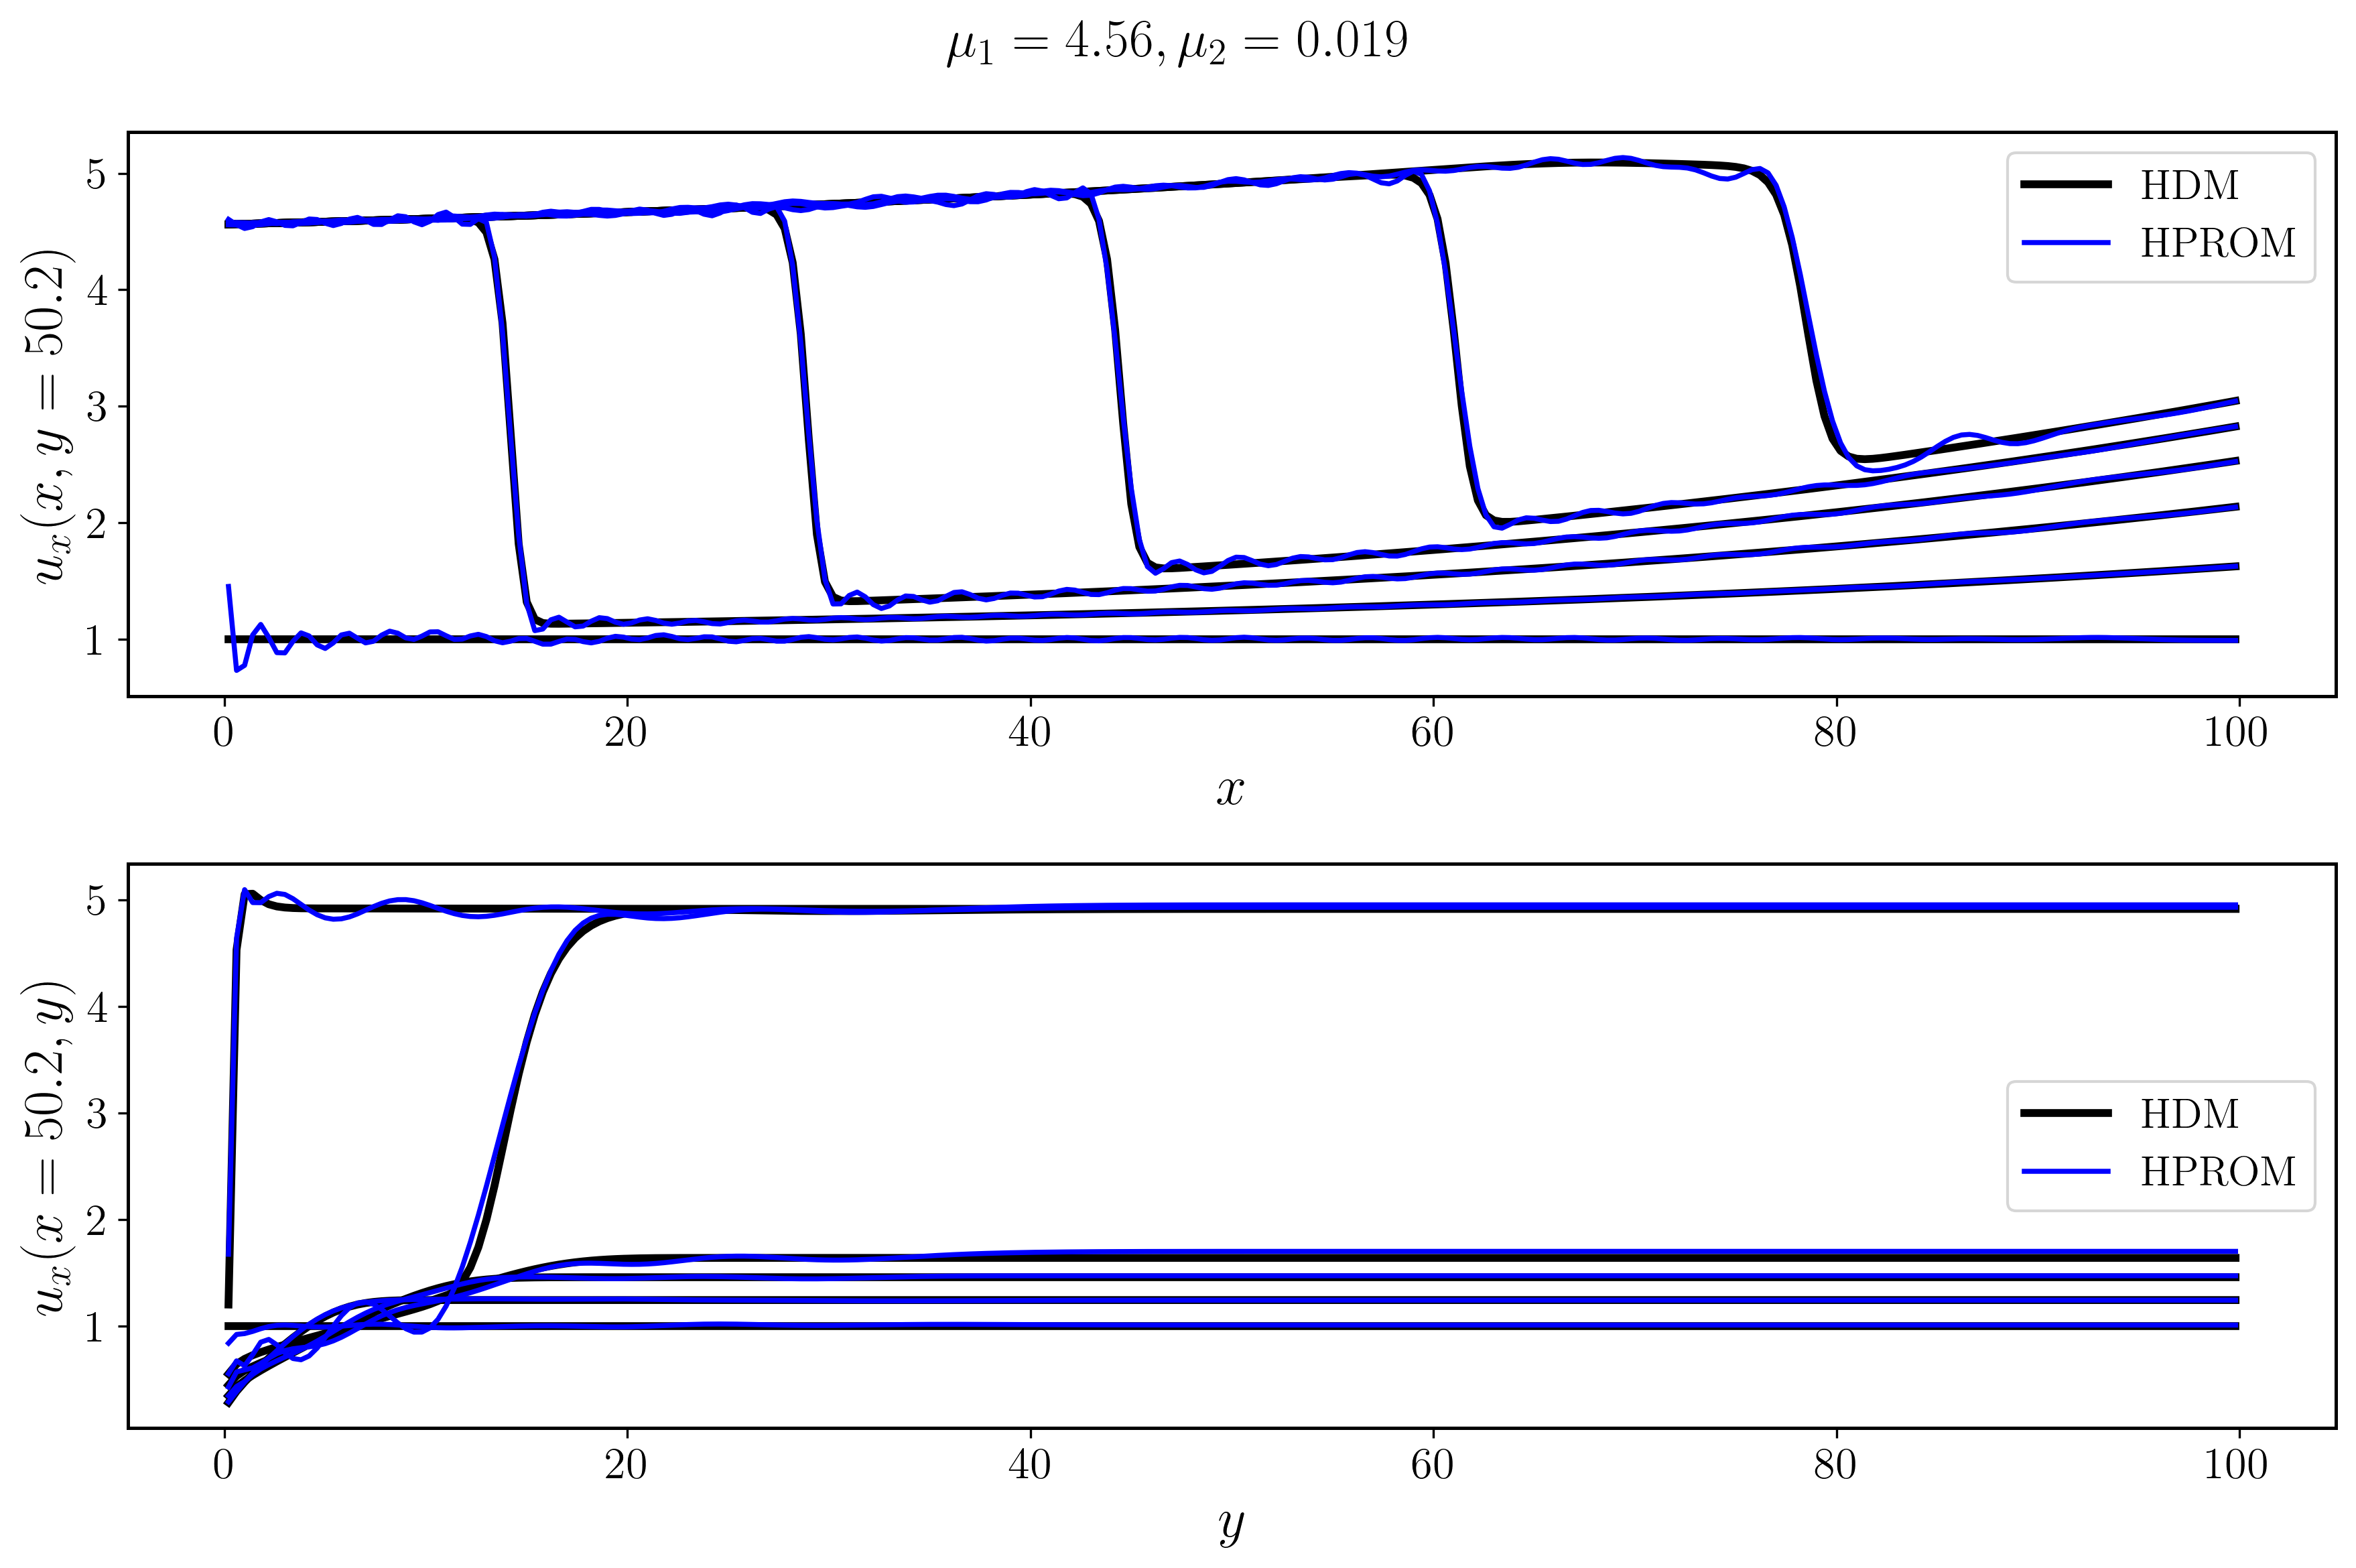
\includegraphics[width=0.82\textwidth,height=0.70\textheight,keepaspectratio]{Figures/hprom_vs_hdm_mu1_4.56_mu2_0.019.png}
\end{frame}

\begin{frame}{HPROM vs HDM: $\boldsymbol\mu=(4.75,\,0.020)$}
\centering
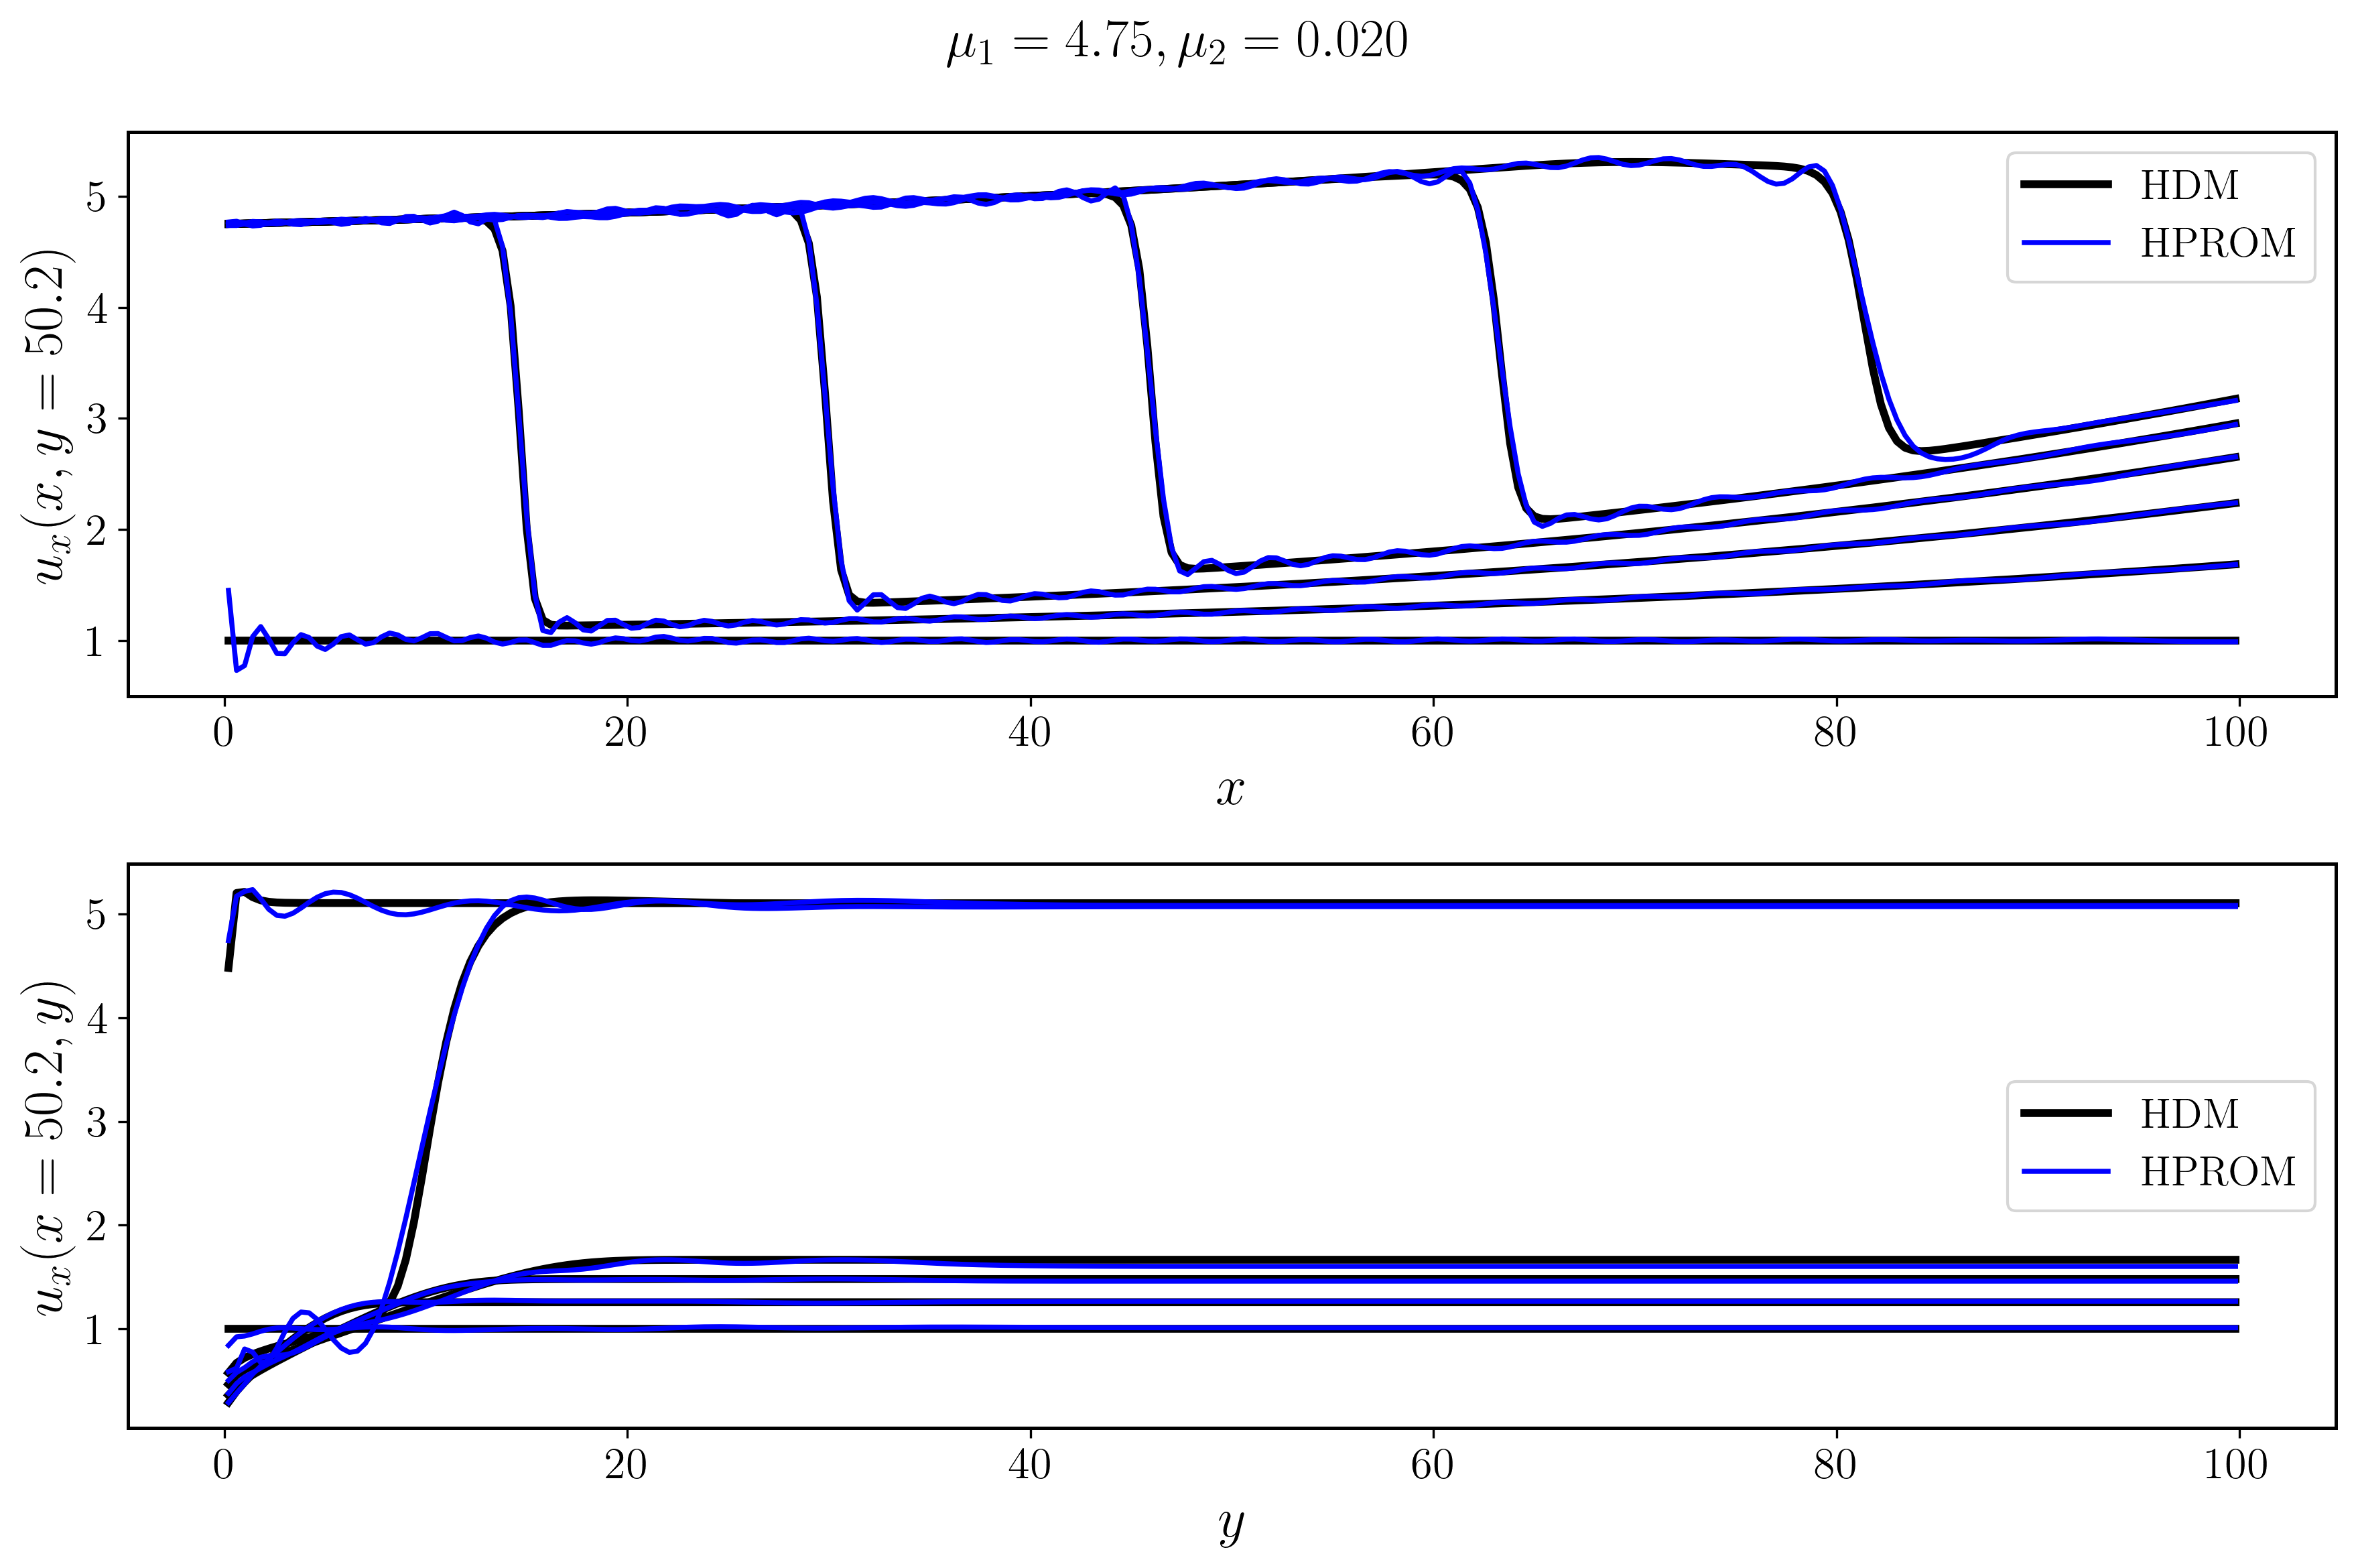
\includegraphics[width=0.82\textwidth,height=0.70\textheight,keepaspectratio]{Figures/hprom_vs_hdm_mu1_4.75_mu2_0.020.png}
\end{frame}

\begin{frame}{HPROM vs HDM: $\boldsymbol\mu=(5.19,\,0.026)$}
\centering
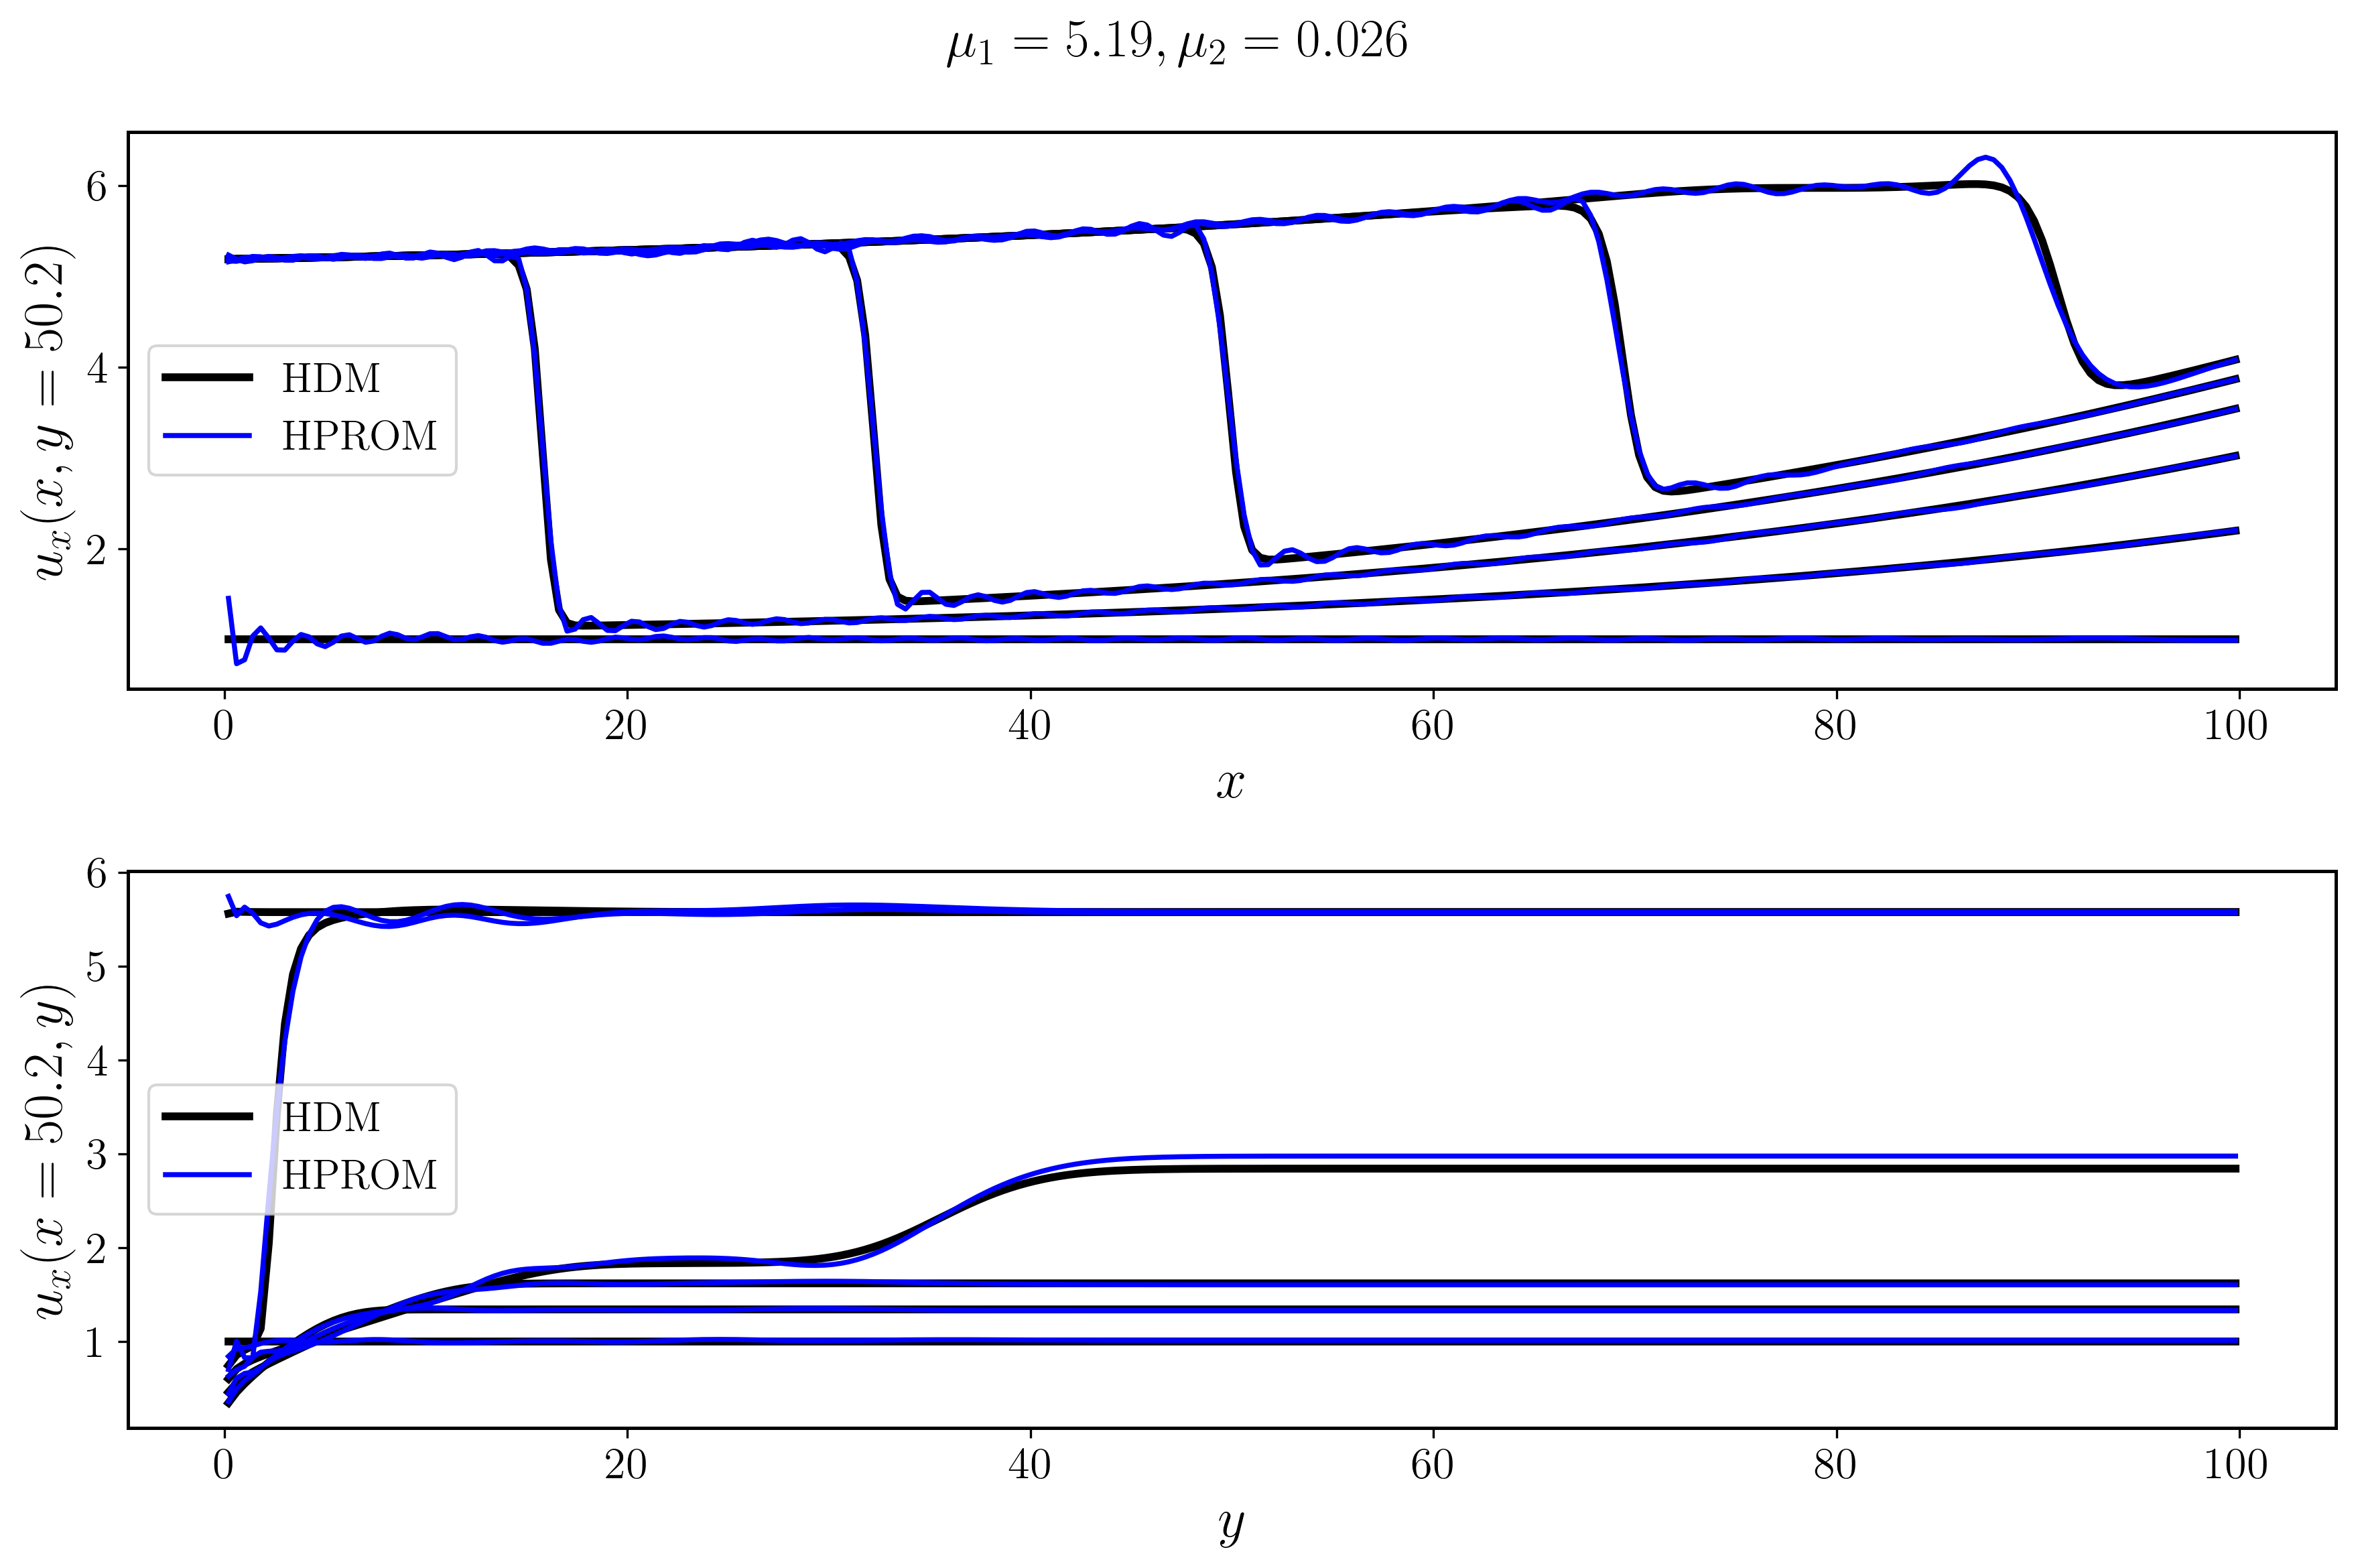
\includegraphics[width=0.82\textwidth,height=0.70\textheight,keepaspectratio]{Figures/hprom_vs_hdm_mu1_5.19_mu2_0.026.png}
\end{frame}

\begin{frame}{Local HPROM ($N_c=3$) vs HDM: $\boldsymbol\mu=(4.56,\,0.019)$}
\centering
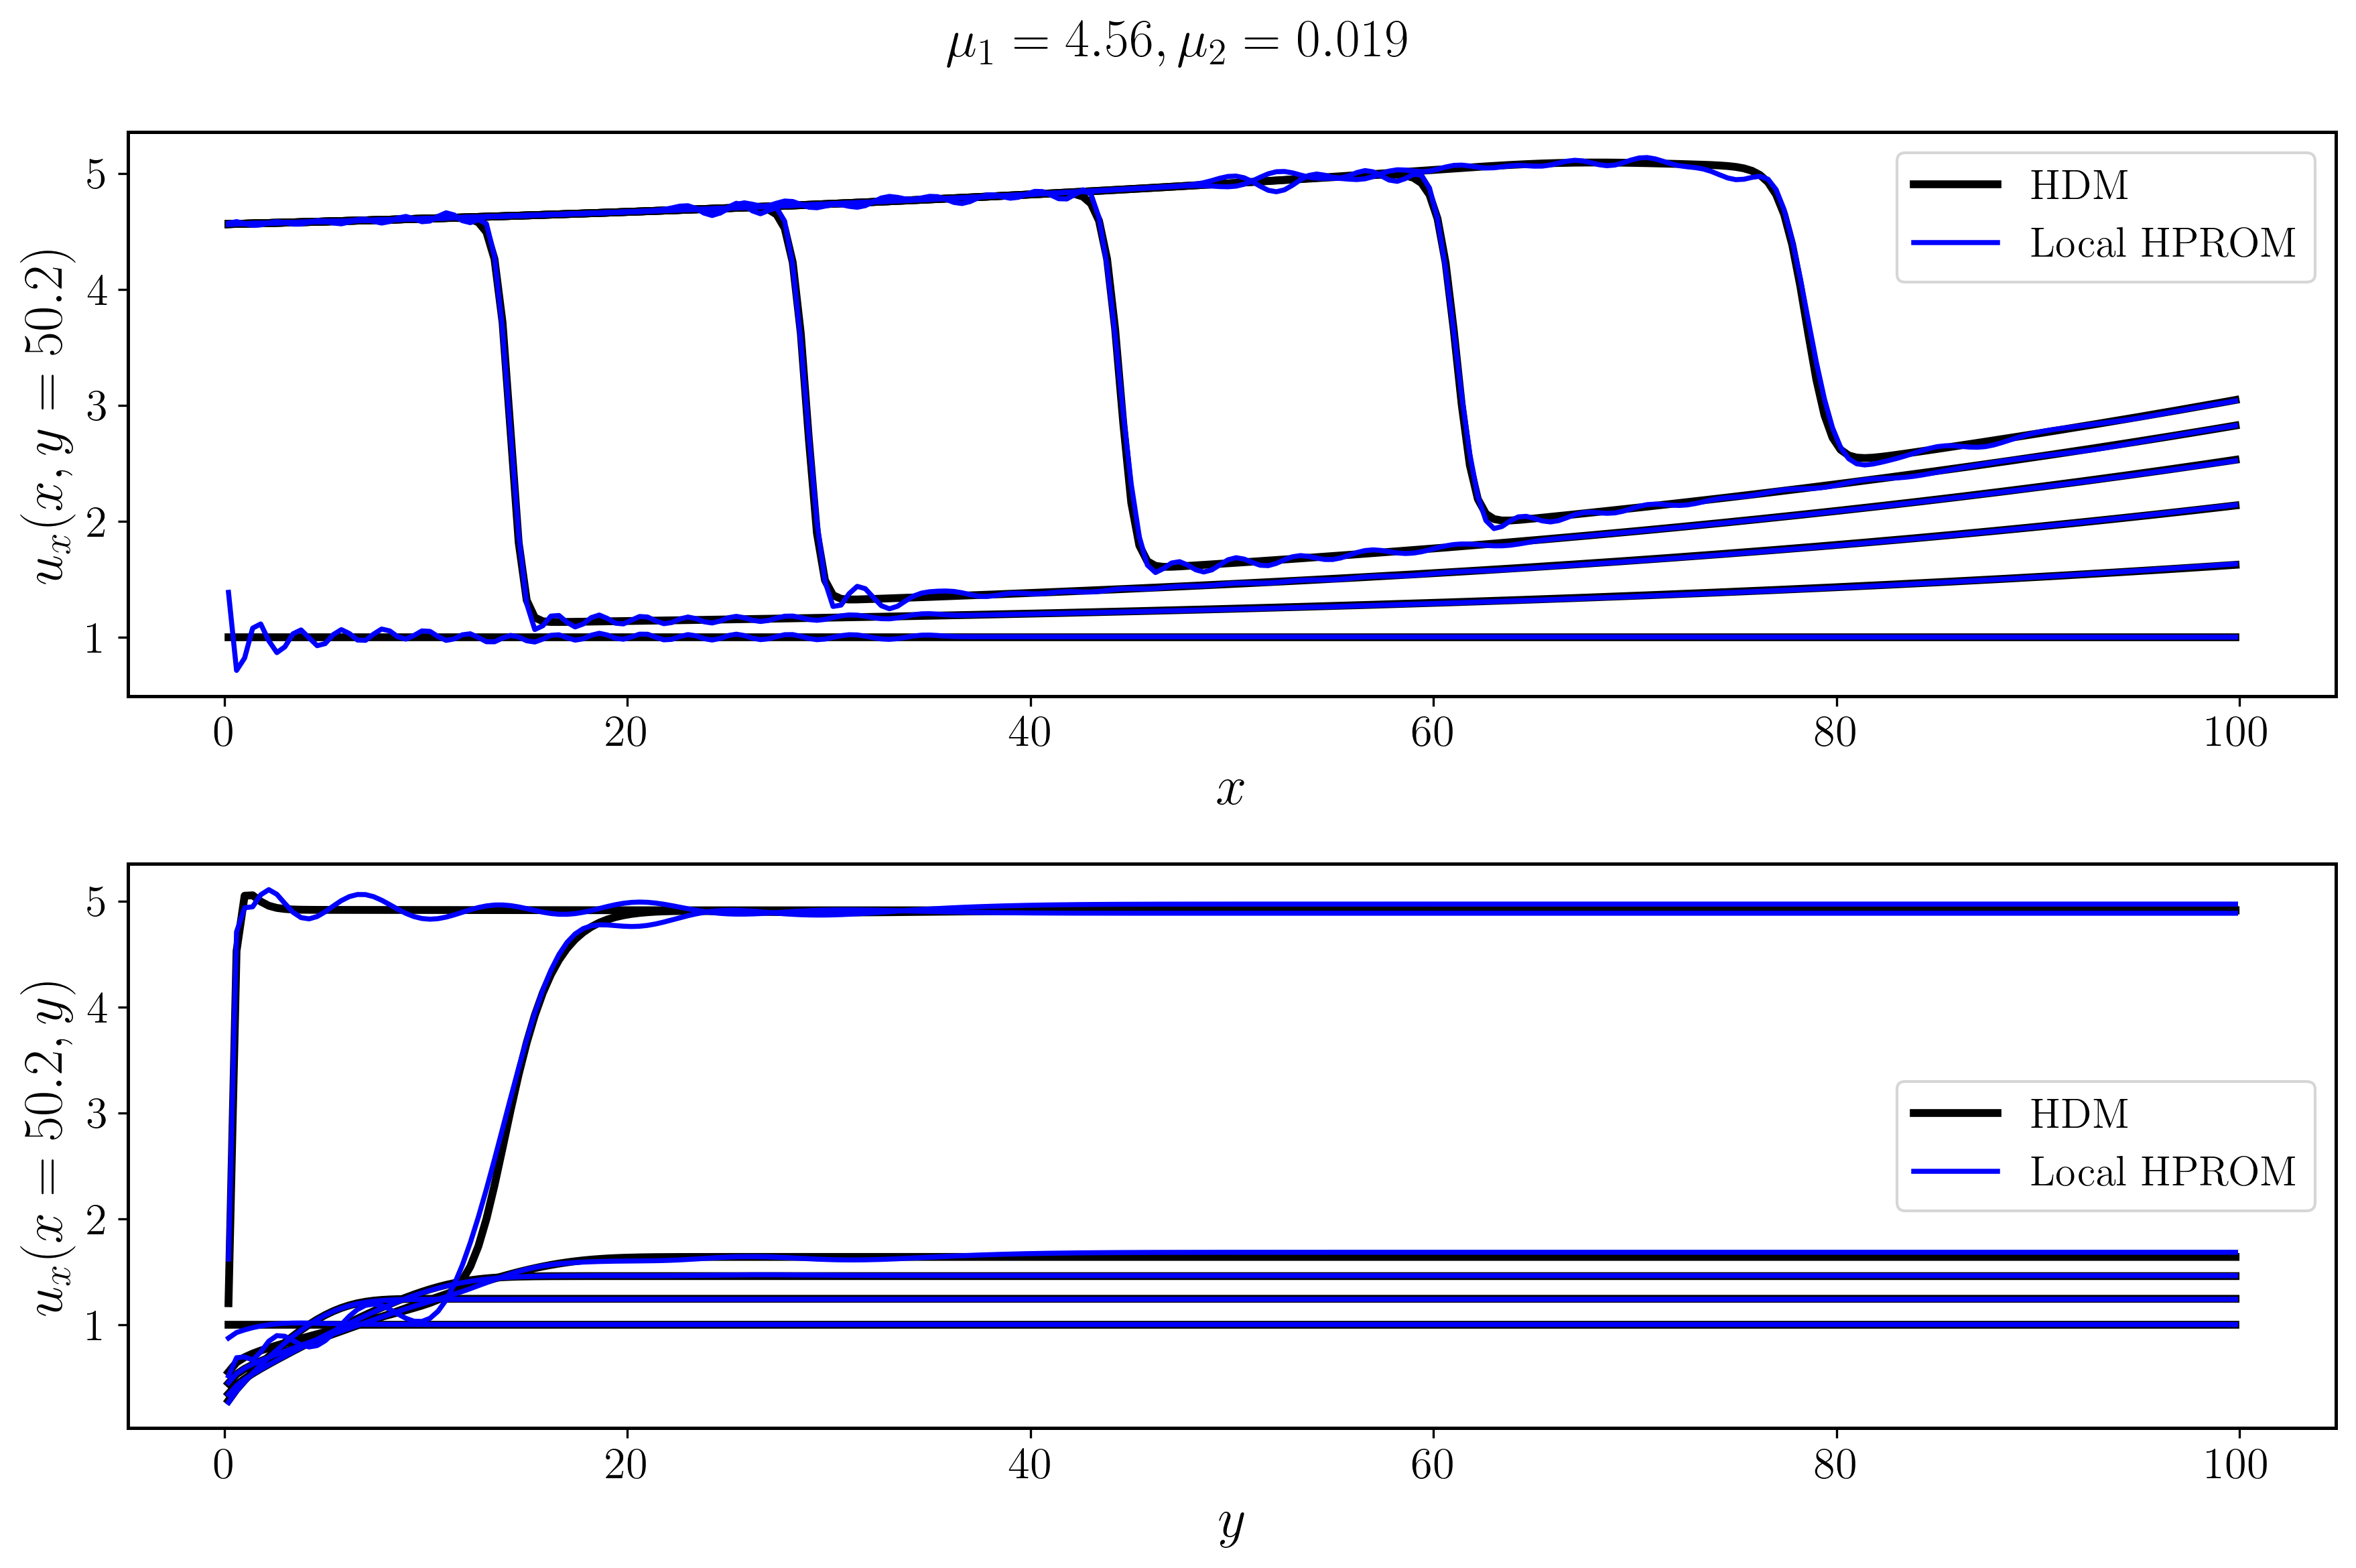
\includegraphics[width=0.82\textwidth,height=0.70\textheight,keepaspectratio]{Figures/local_hprom_vs_hdm_mu1_4.56_mu2_0.019.png}
\end{frame}

\begin{frame}{Local HPROM ($N_c=3$) vs HDM: $\boldsymbol\mu=(4.75,\,0.020)$}
\centering
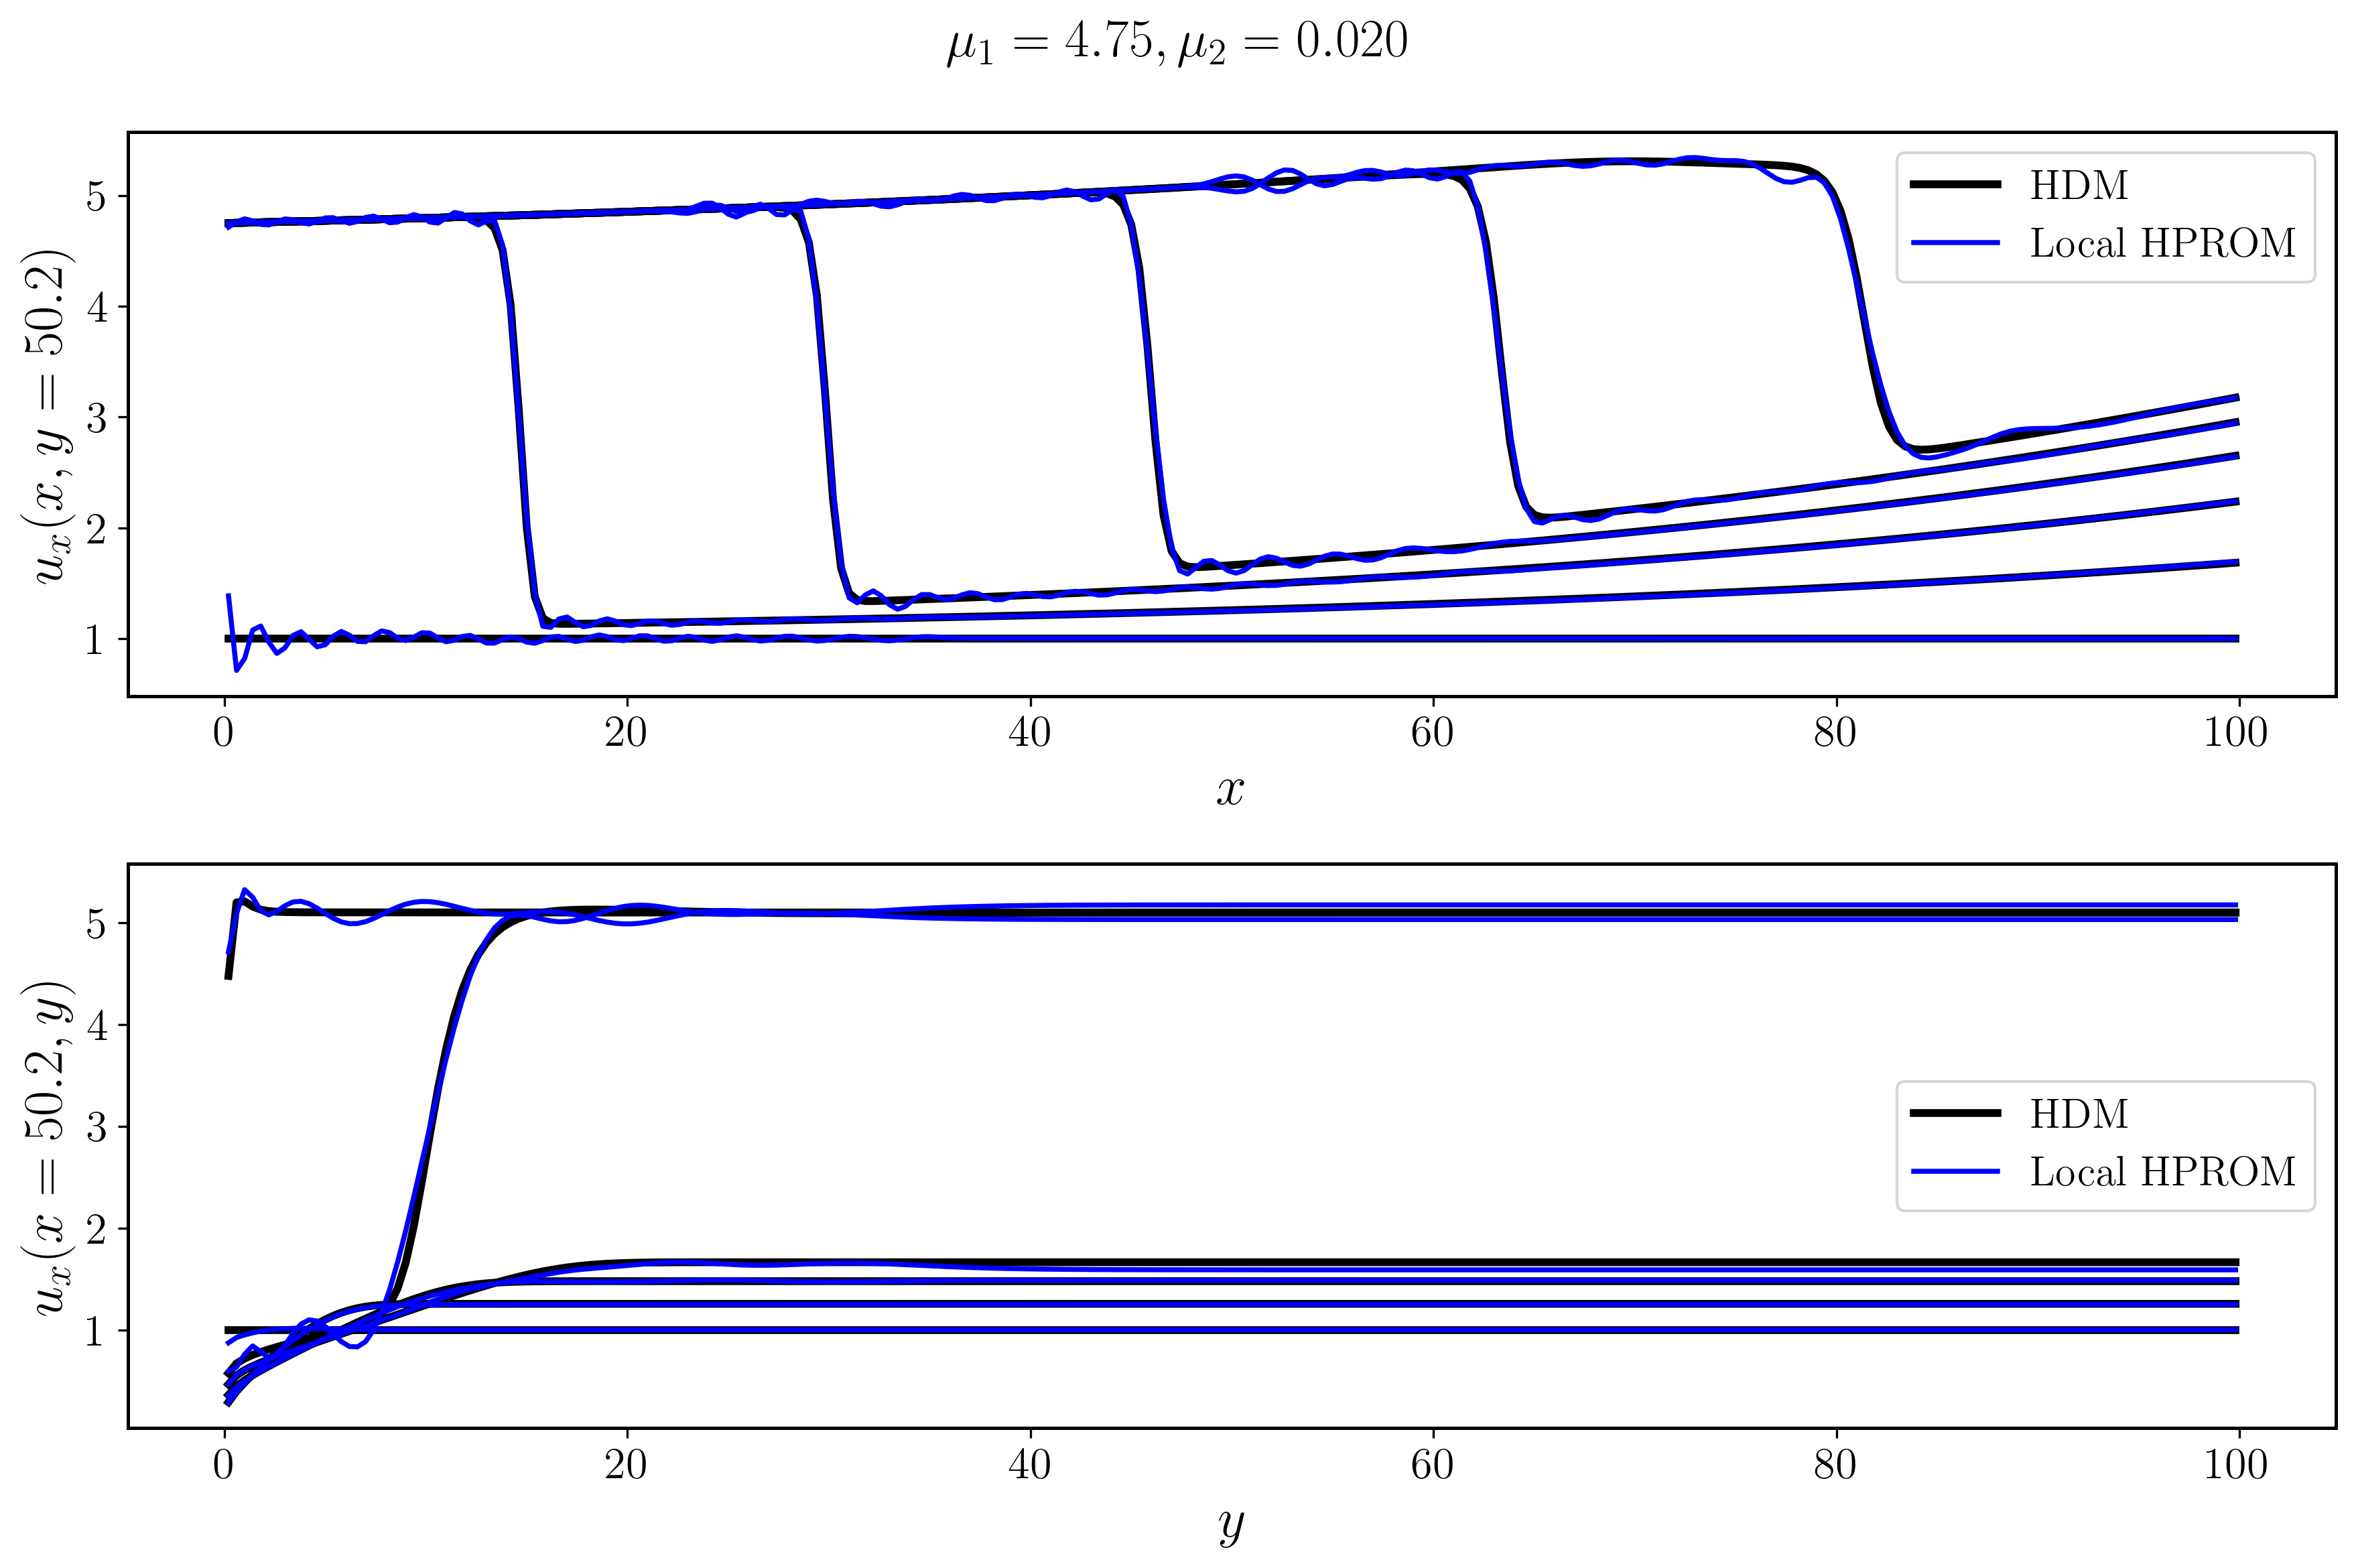
\includegraphics[width=0.82\textwidth,height=0.70\textheight,keepaspectratio]{Figures/local_hprom_vs_hdm_mu1_4.75_mu2_0.020.png}
\end{frame}

\begin{frame}{Local HPROM ($N_c=3$) vs HDM: $\boldsymbol\mu=(5.19,\,0.026)$}
\centering
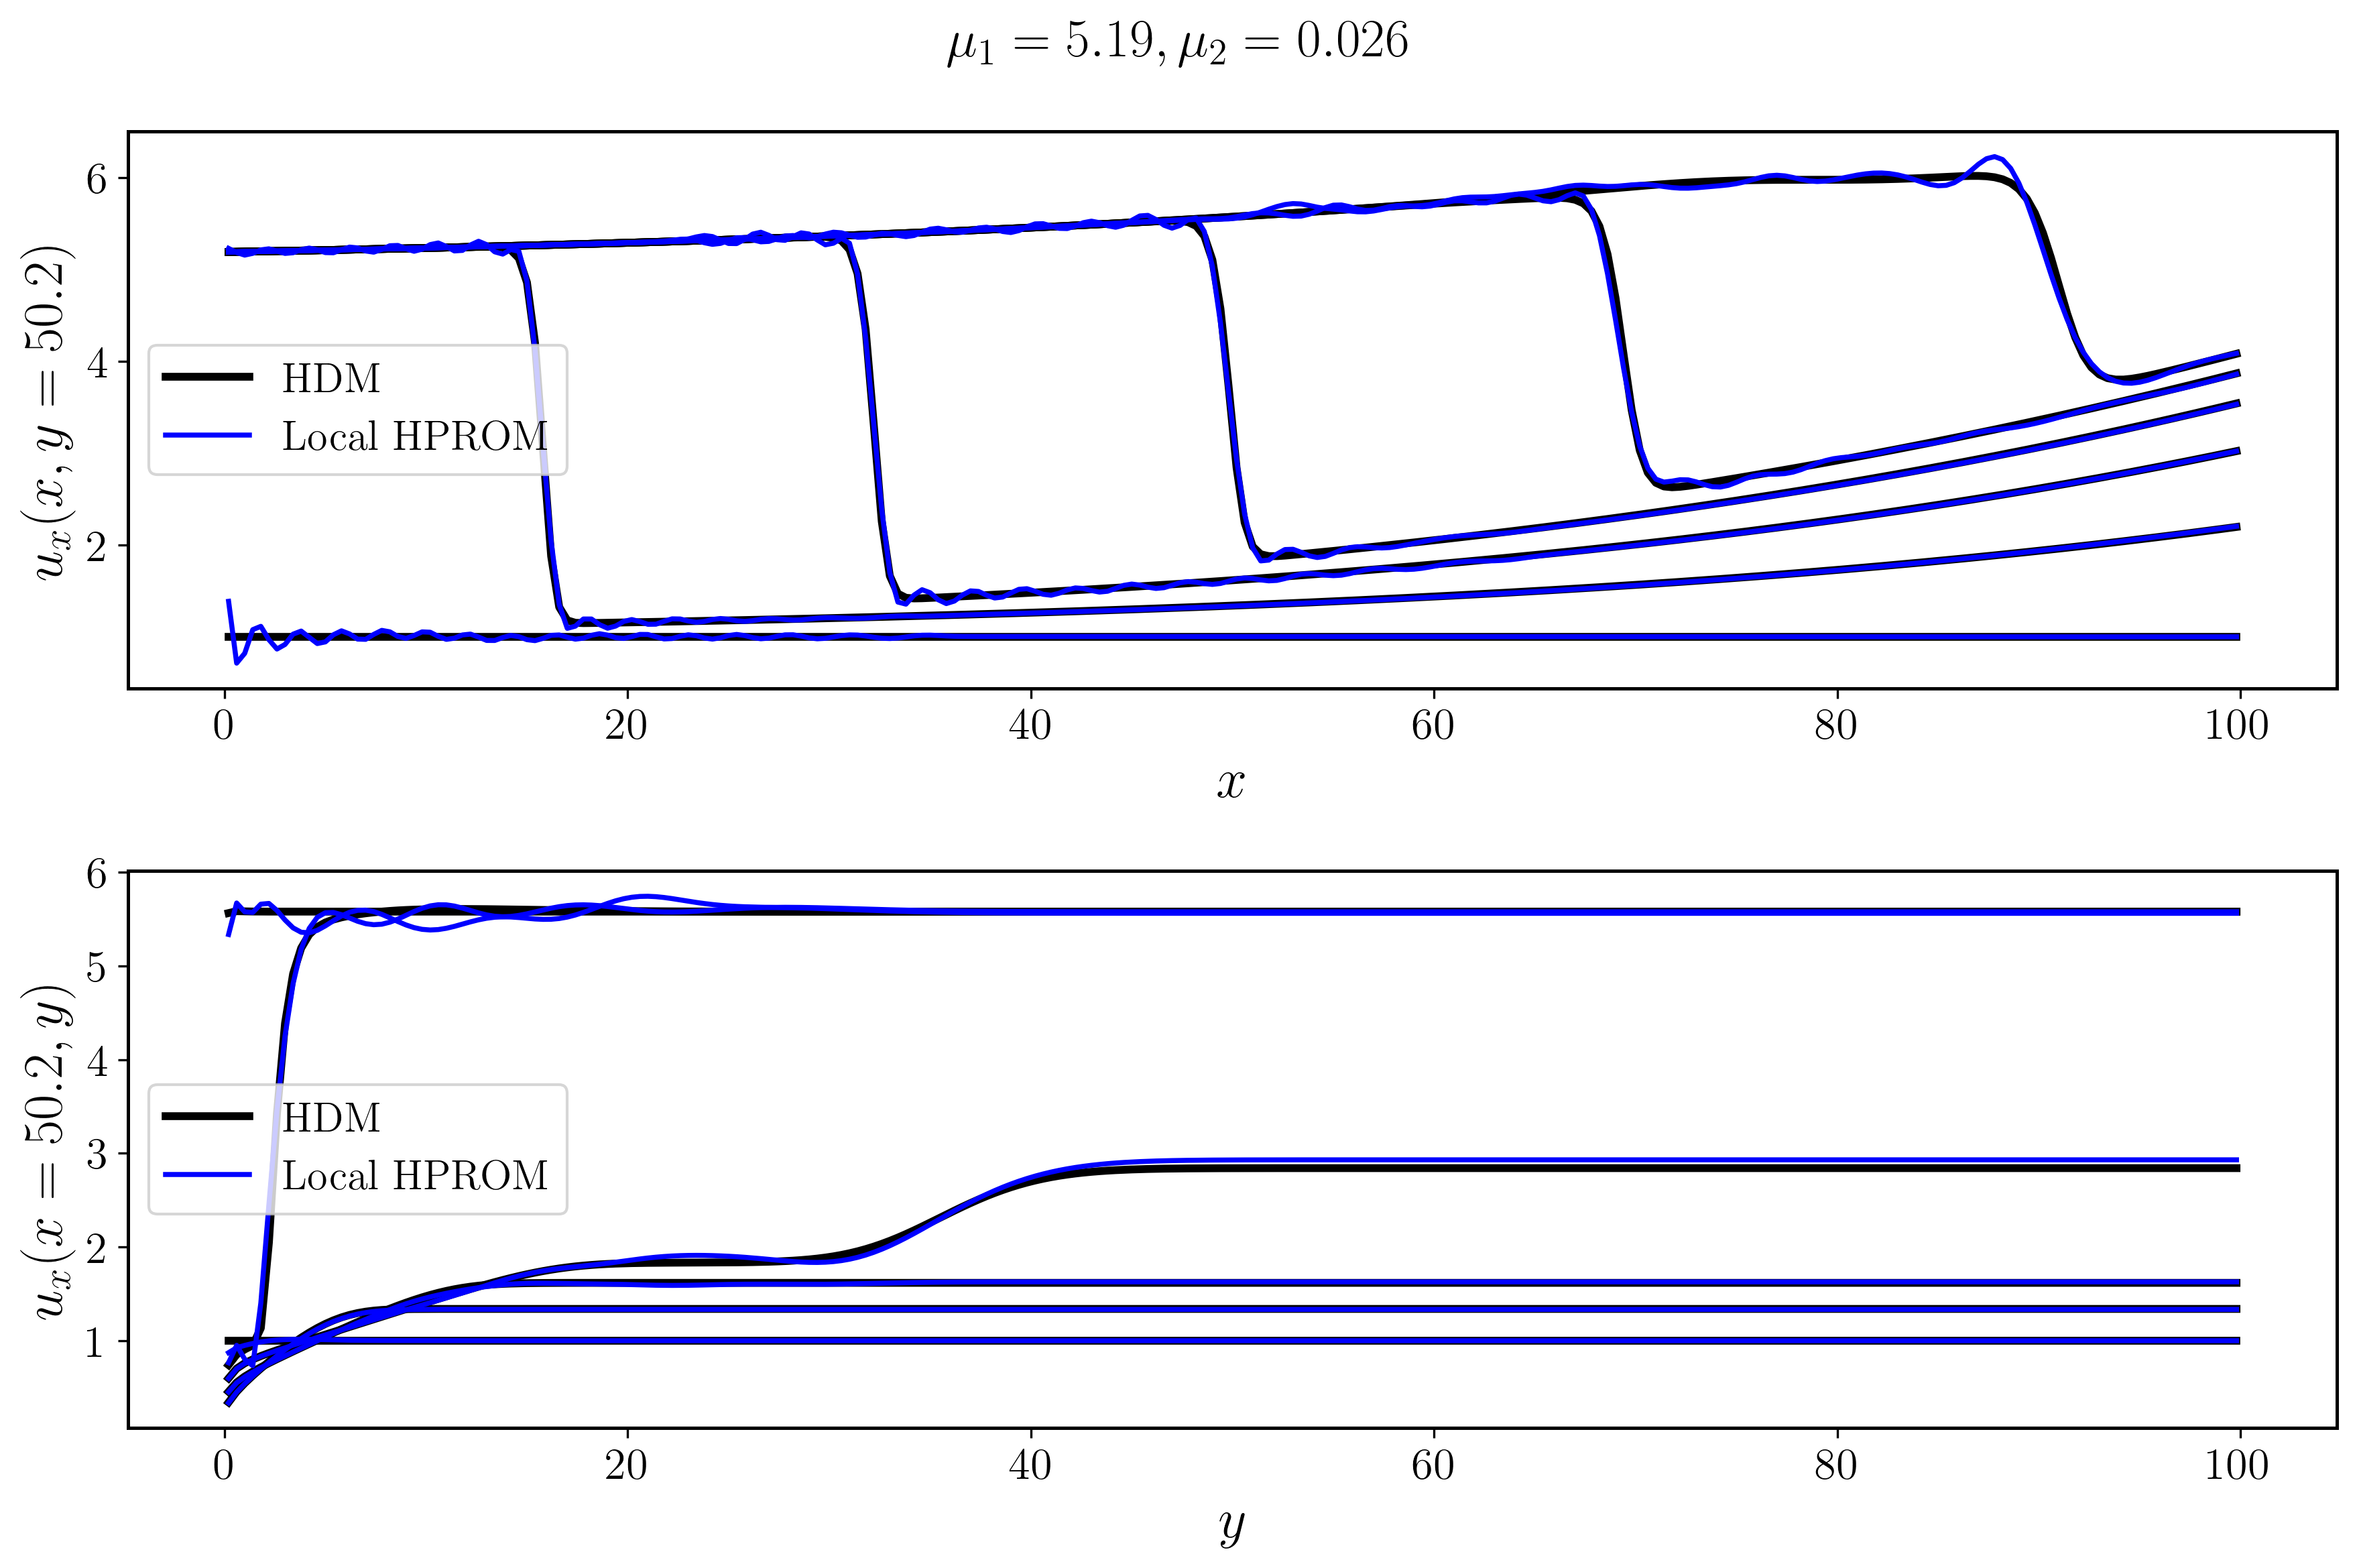
\includegraphics[width=0.82\textwidth,height=0.70\textheight,keepaspectratio]{Figures/local_hprom_vs_hdm_mu1_5.19_mu2_0.026.png}
\end{frame}

\begin{frame}{HQPROM vs HDM: $\boldsymbol\mu=(4.56,\,0.019)$}
\centering
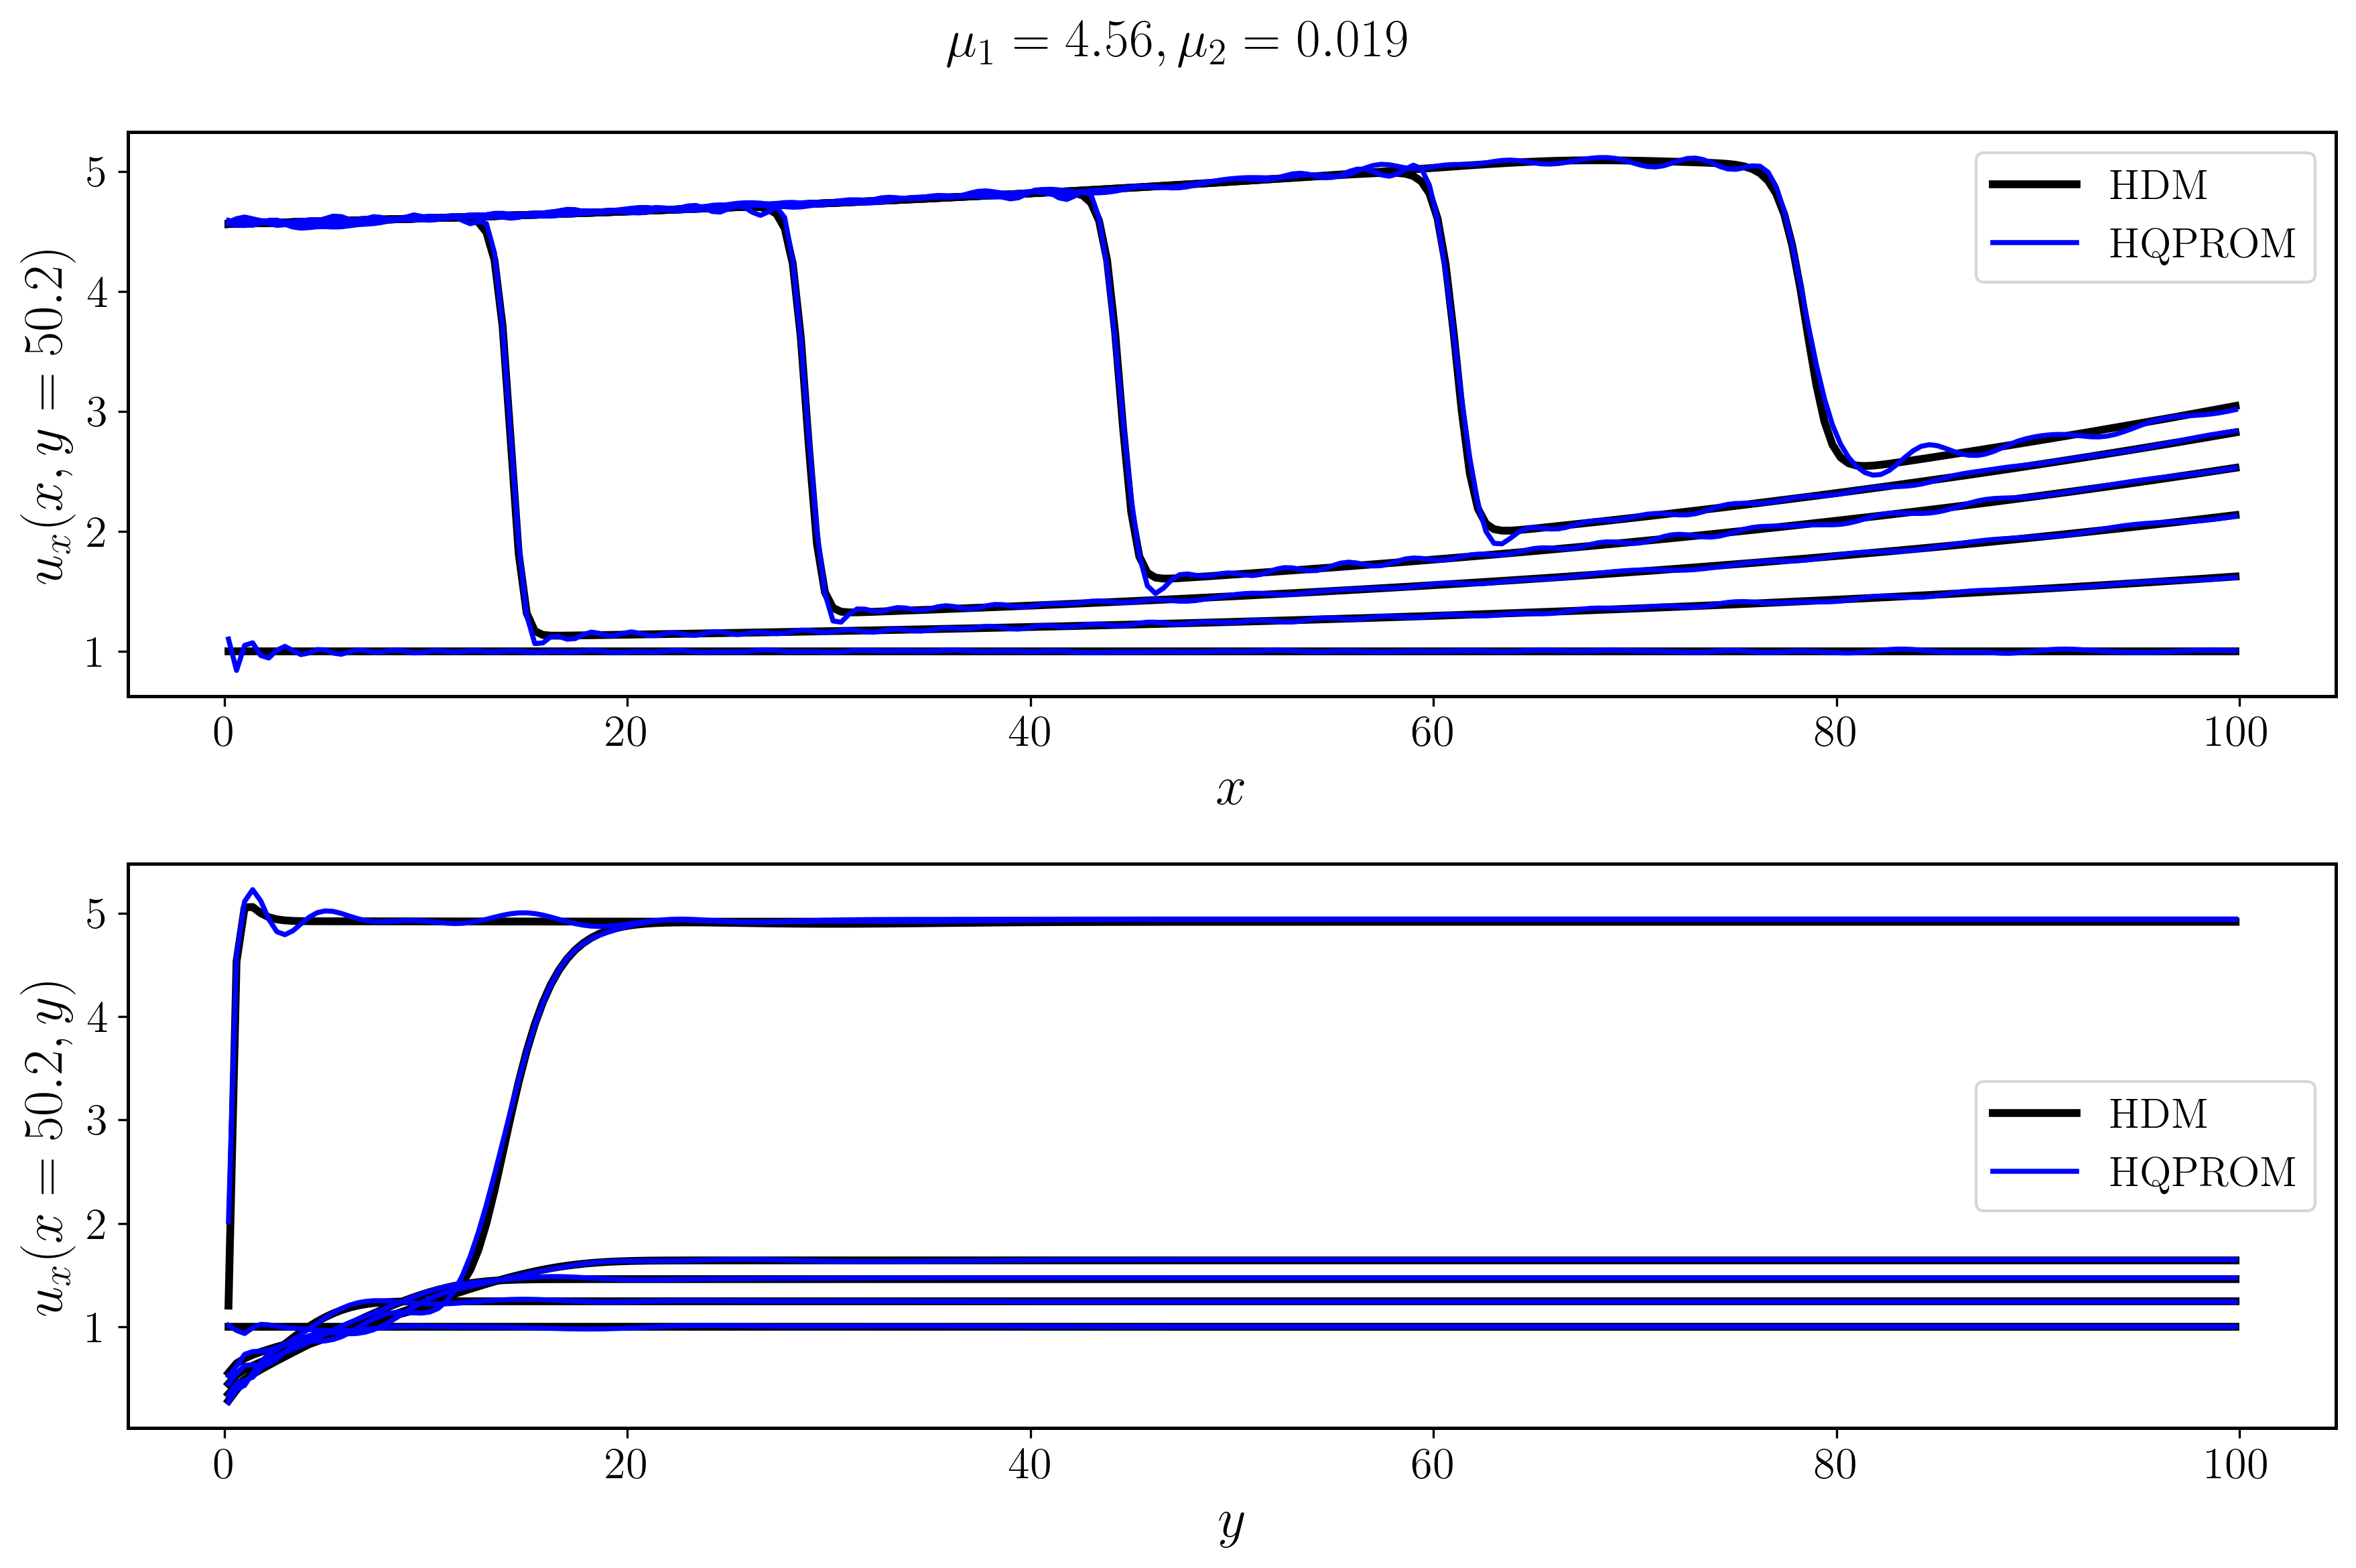
\includegraphics[width=0.82\textwidth,height=0.70\textheight,keepaspectratio]{Figures/hqprom_vs_hdm_mu1_4.56_mu2_0.019.png}
\end{frame}

\begin{frame}{HQPROM vs HDM: $\boldsymbol\mu=(4.75,\,0.020)$}
\centering
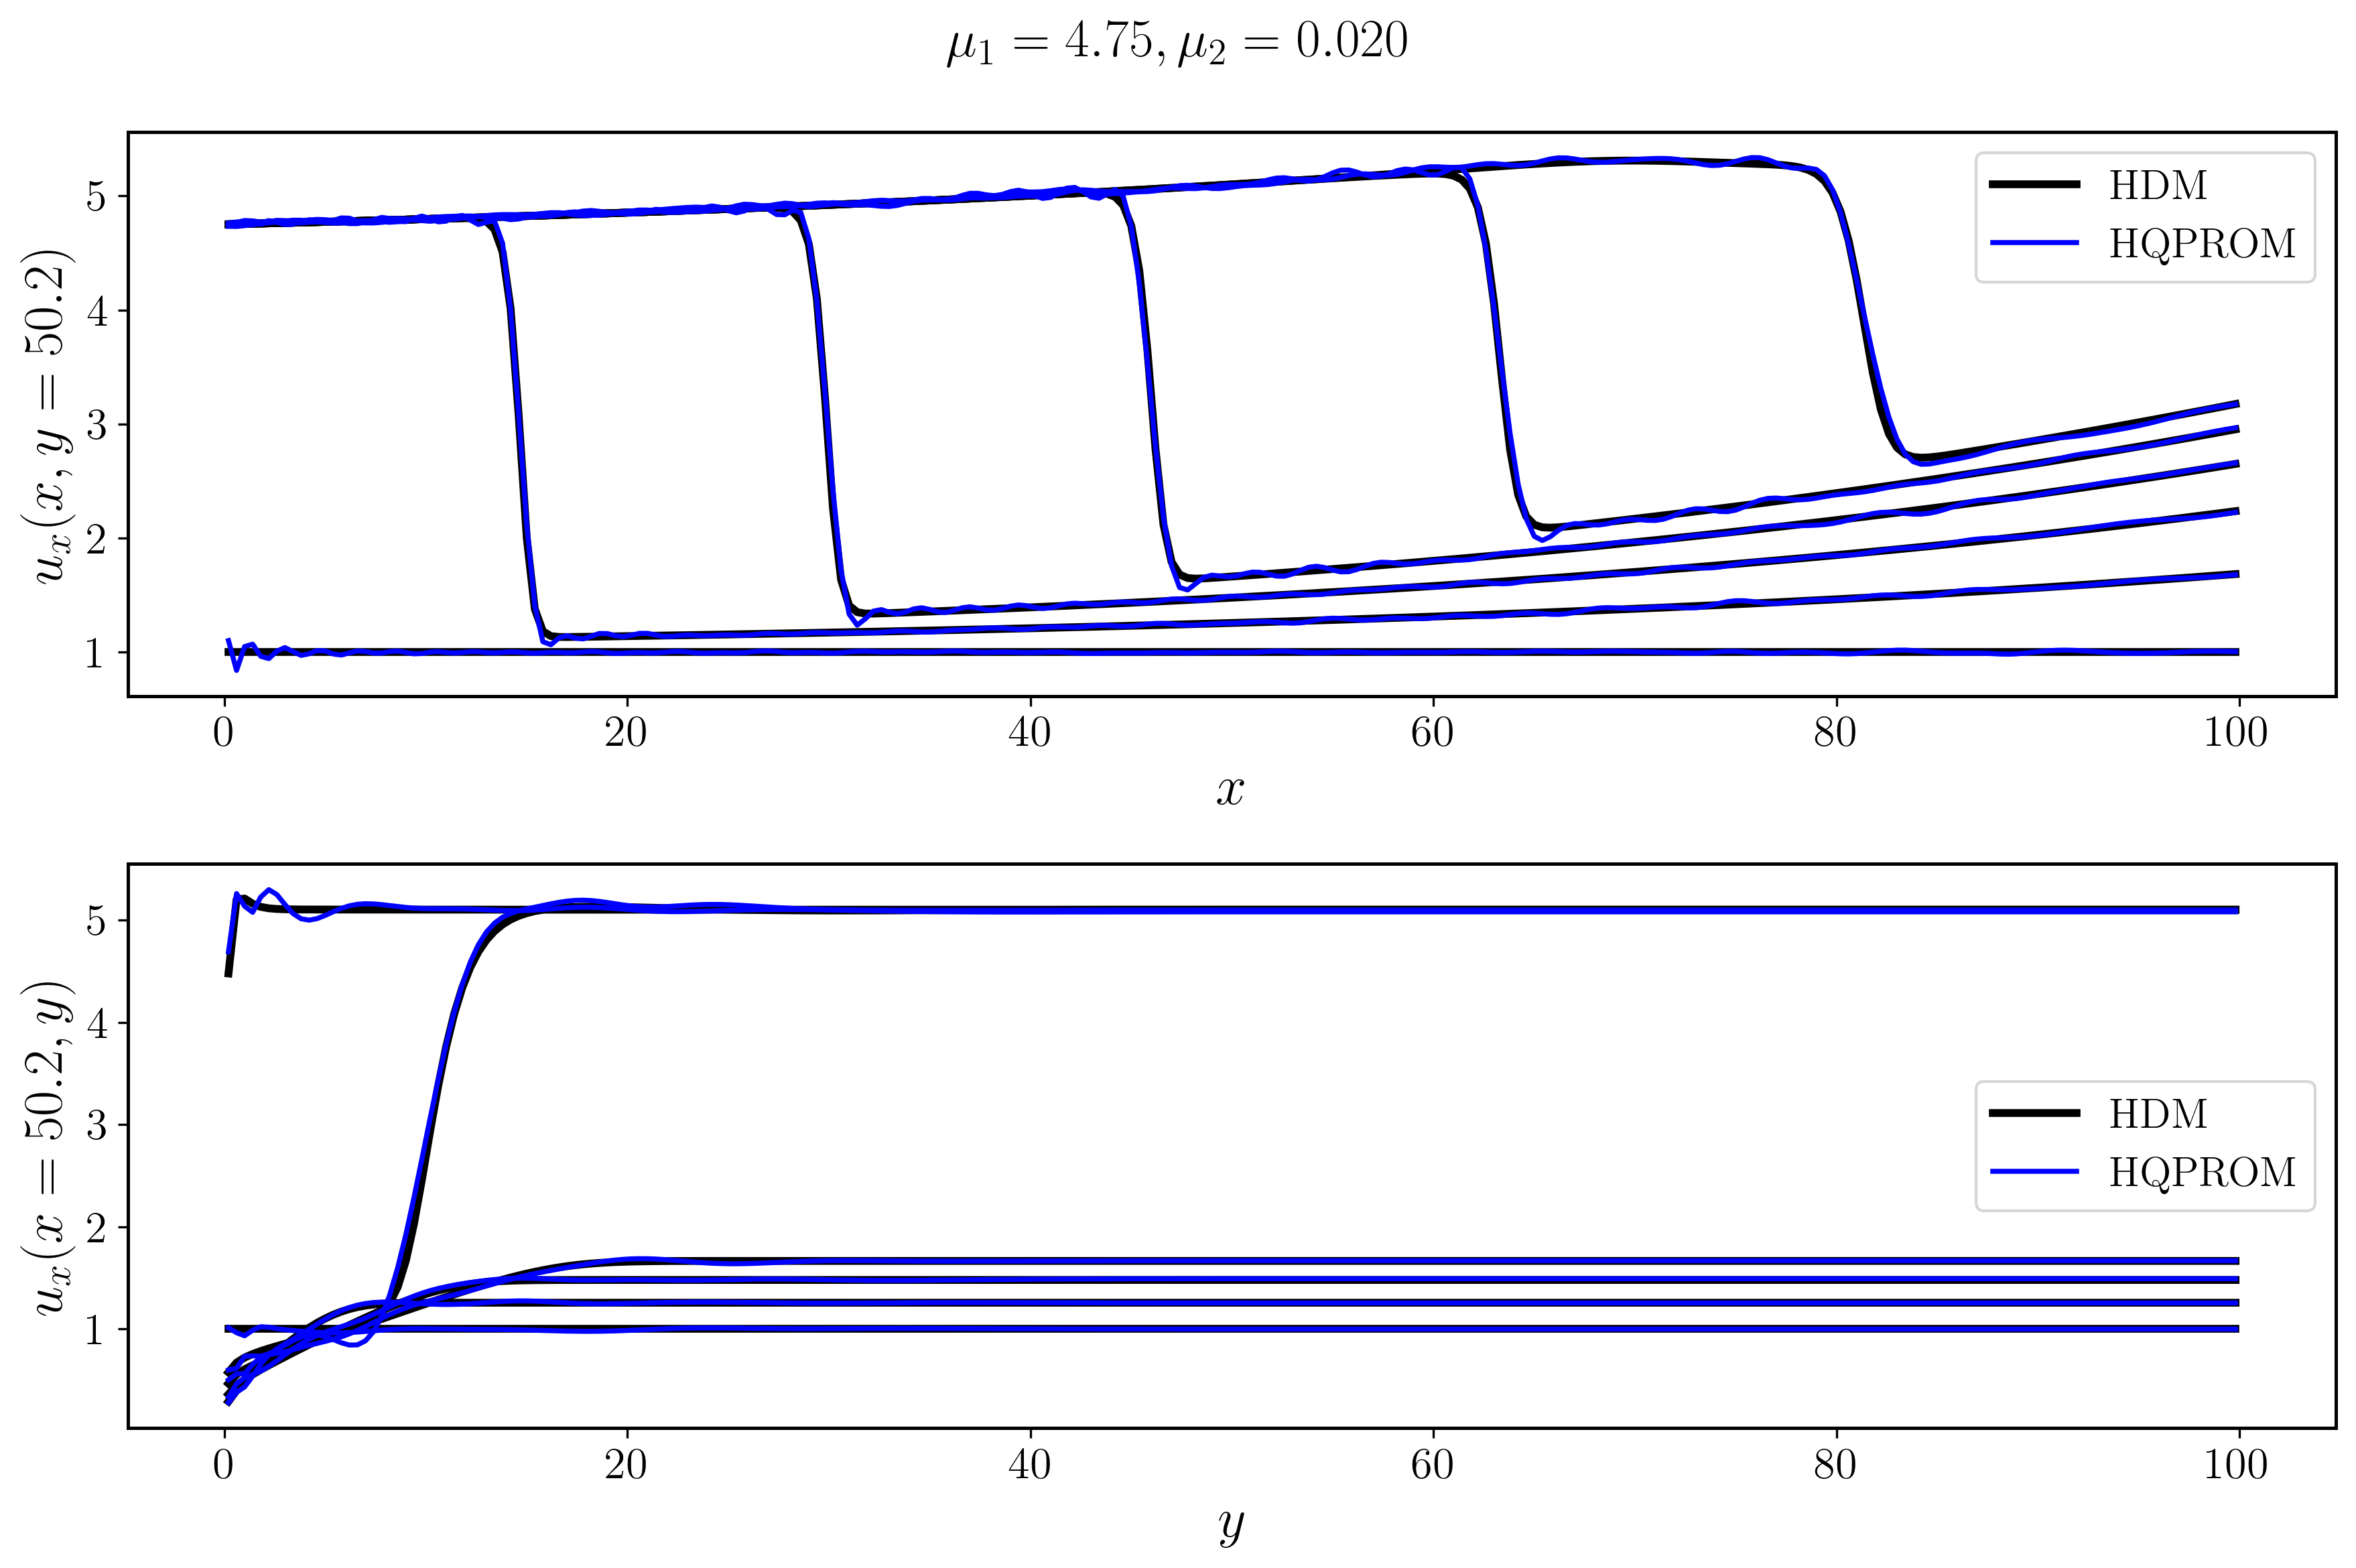
\includegraphics[width=0.82\textwidth,height=0.70\textheight,keepaspectratio]{Figures/hqprom_vs_hdm_mu1_4.75_mu2_0.020.png}
\end{frame}

\begin{frame}{HQPROM vs HDM: $\boldsymbol\mu=(5.19,\,0.026)$}
\centering
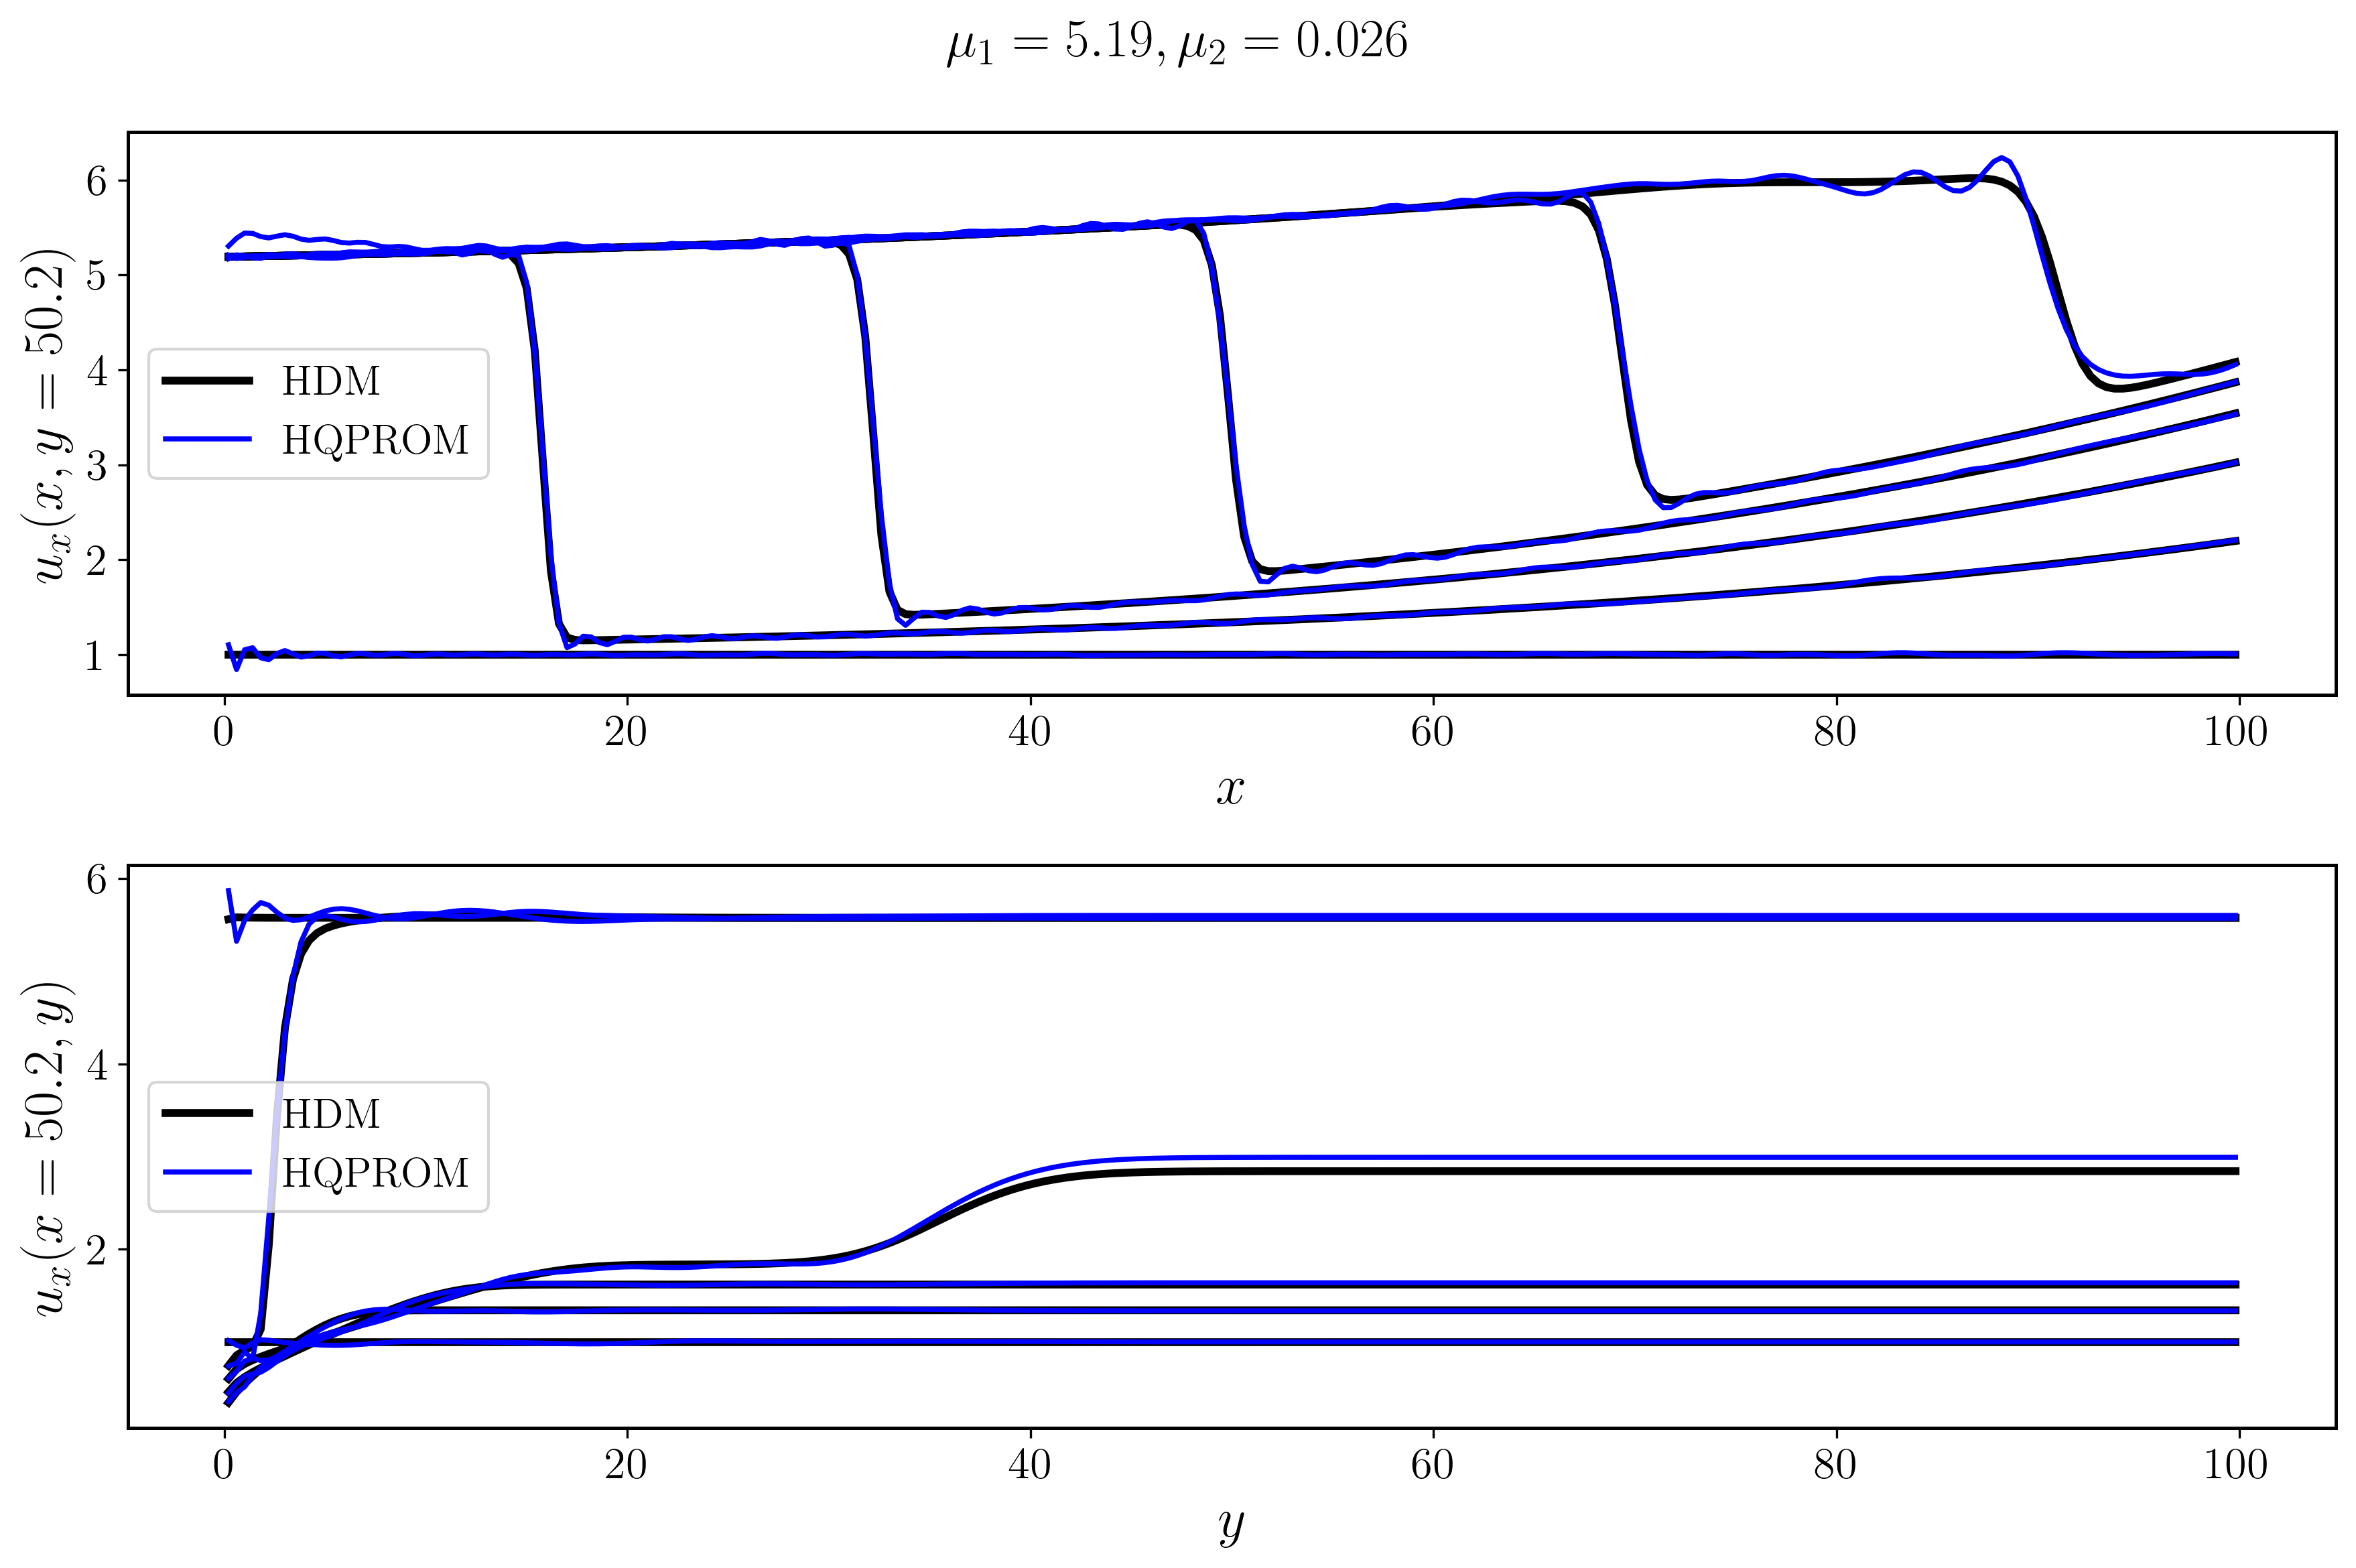
\includegraphics[width=0.82\textwidth,height=0.70\textheight,keepaspectratio]{Figures/hqprom_vs_hdm_mu1_5.19_mu2_0.026.png}
\end{frame}

\begin{frame}{Local HQPROM ($N_c=3$) vs HDM: $\boldsymbol\mu=(4.56,\,0.019)$}
\centering
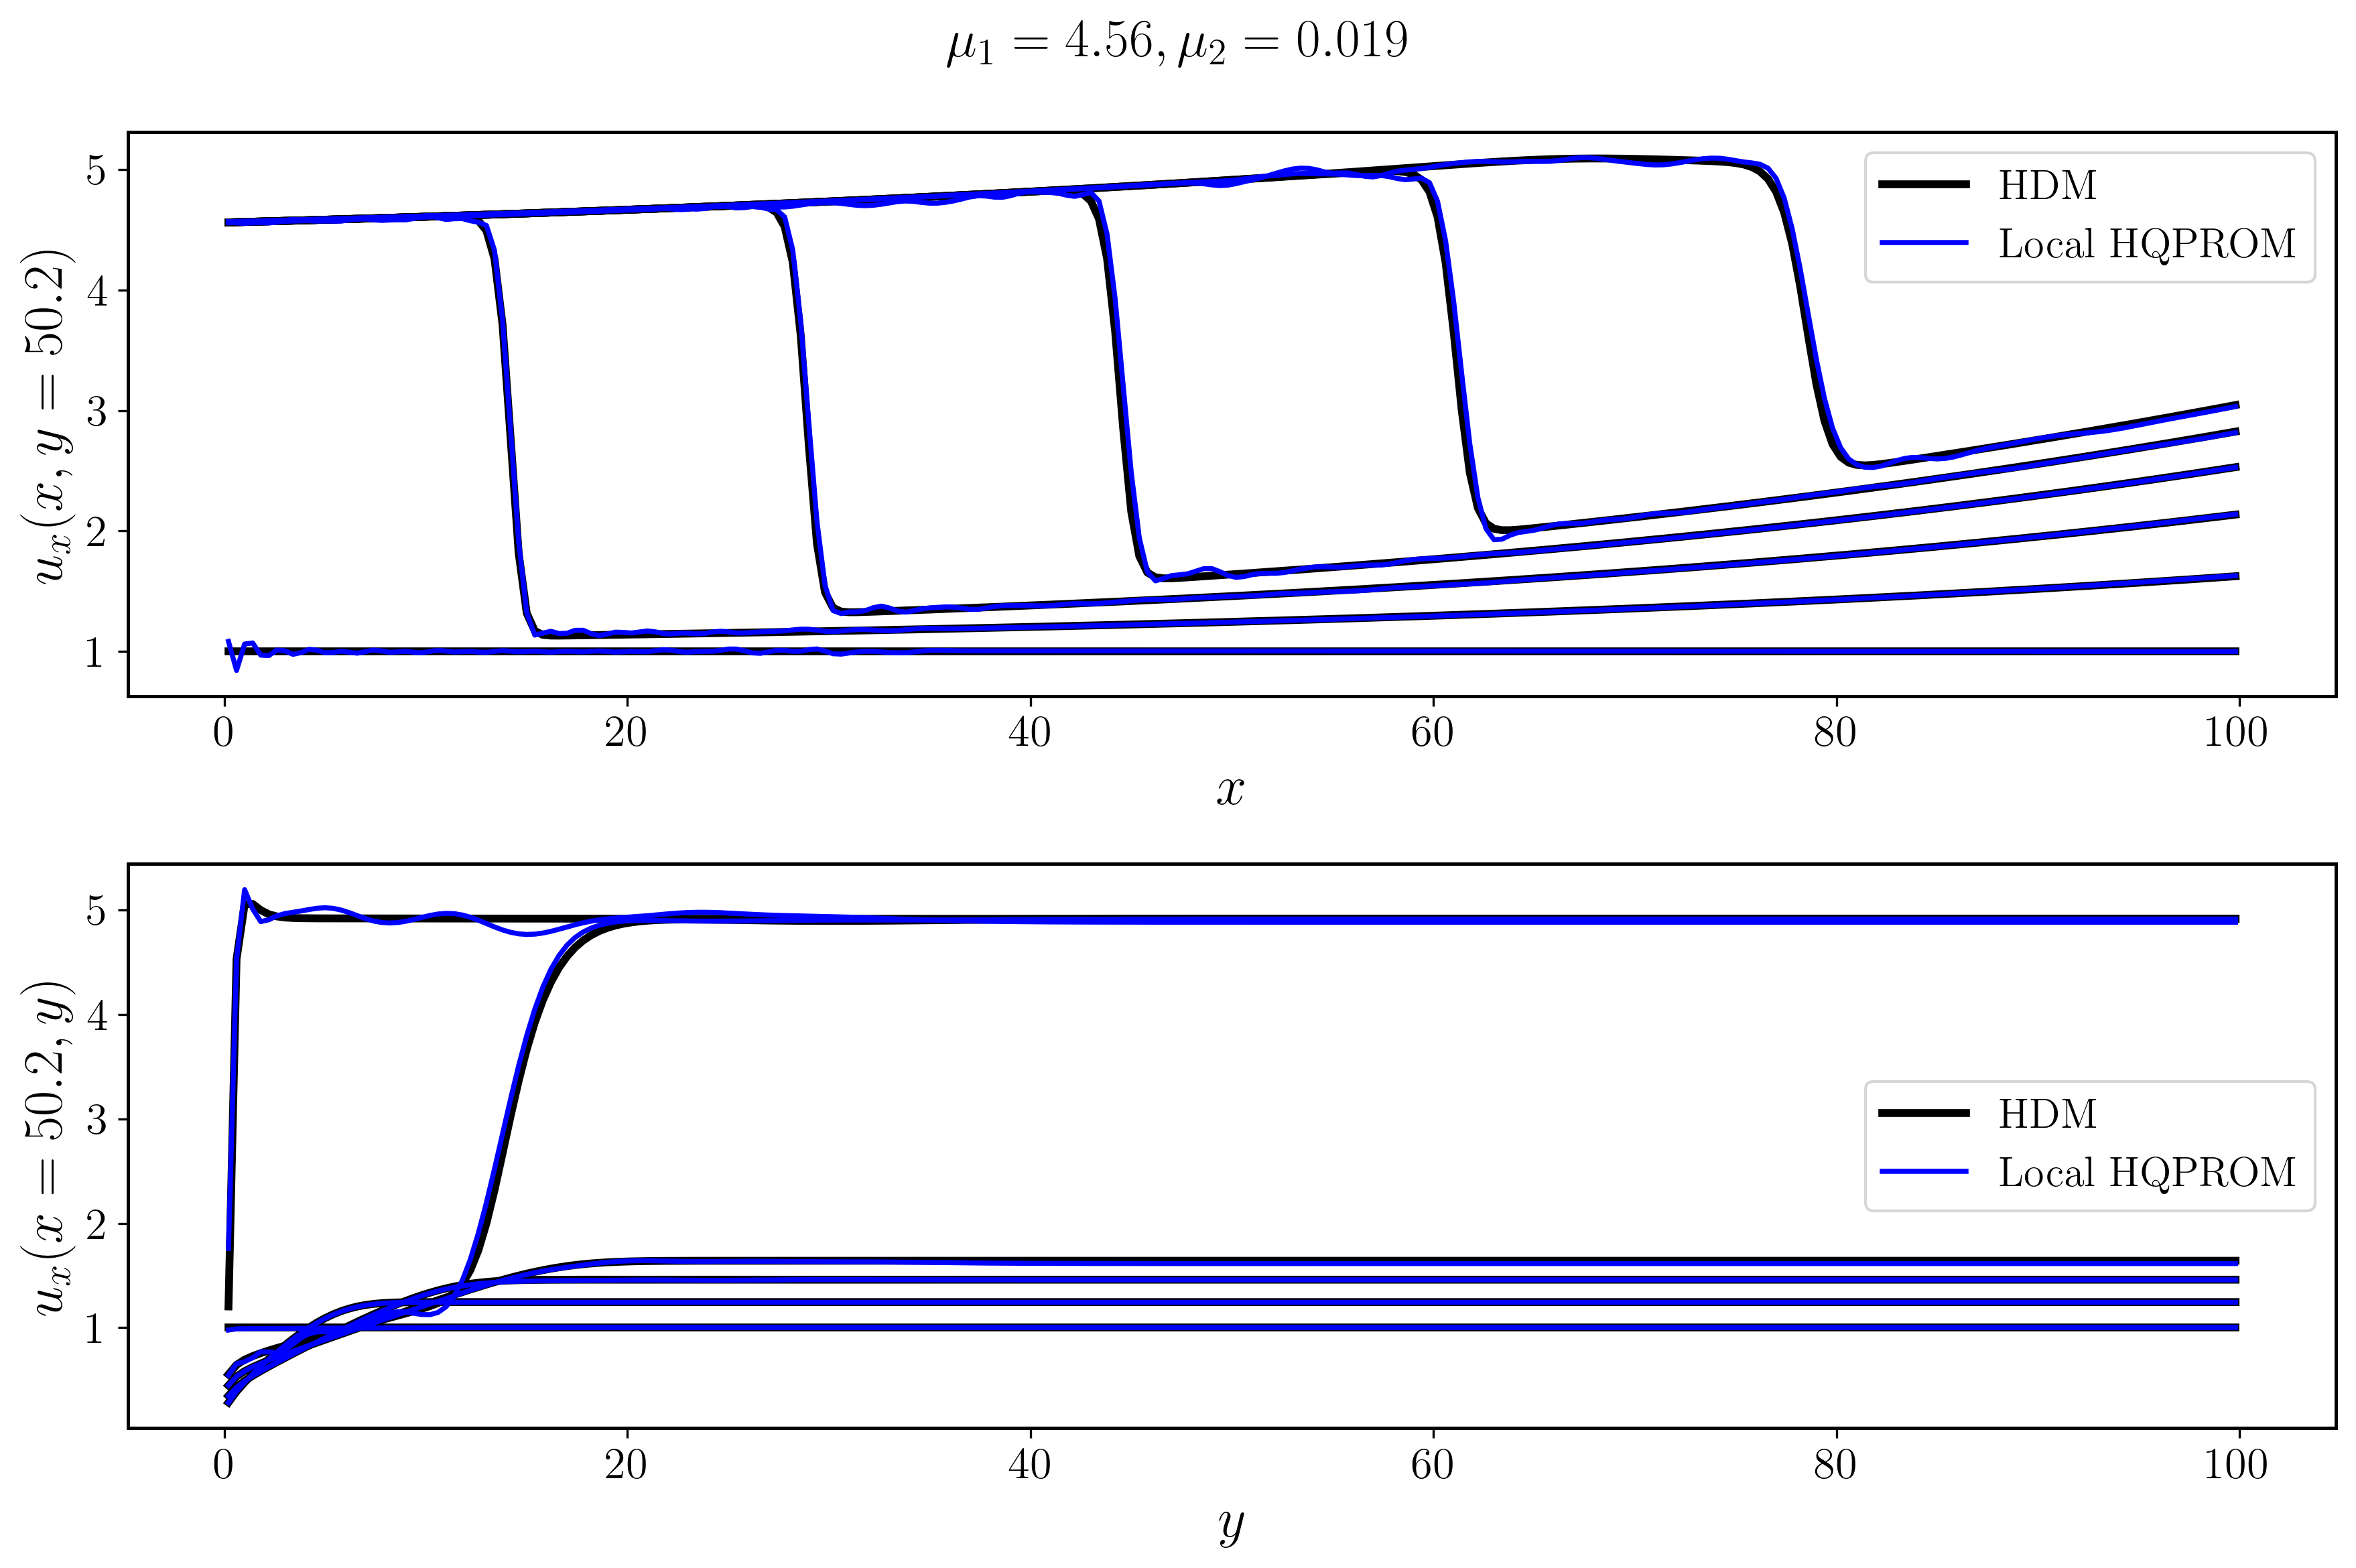
\includegraphics[width=0.82\textwidth,height=0.70\textheight,keepaspectratio]{Figures/local_hqprom_vs_hdm_mu1_4.56_mu2_0.019.png}
\end{frame}

\begin{frame}{Local HQPROM ($N_c=3$) vs HDM: $\boldsymbol\mu=(4.75,\,0.020)$}
\centering
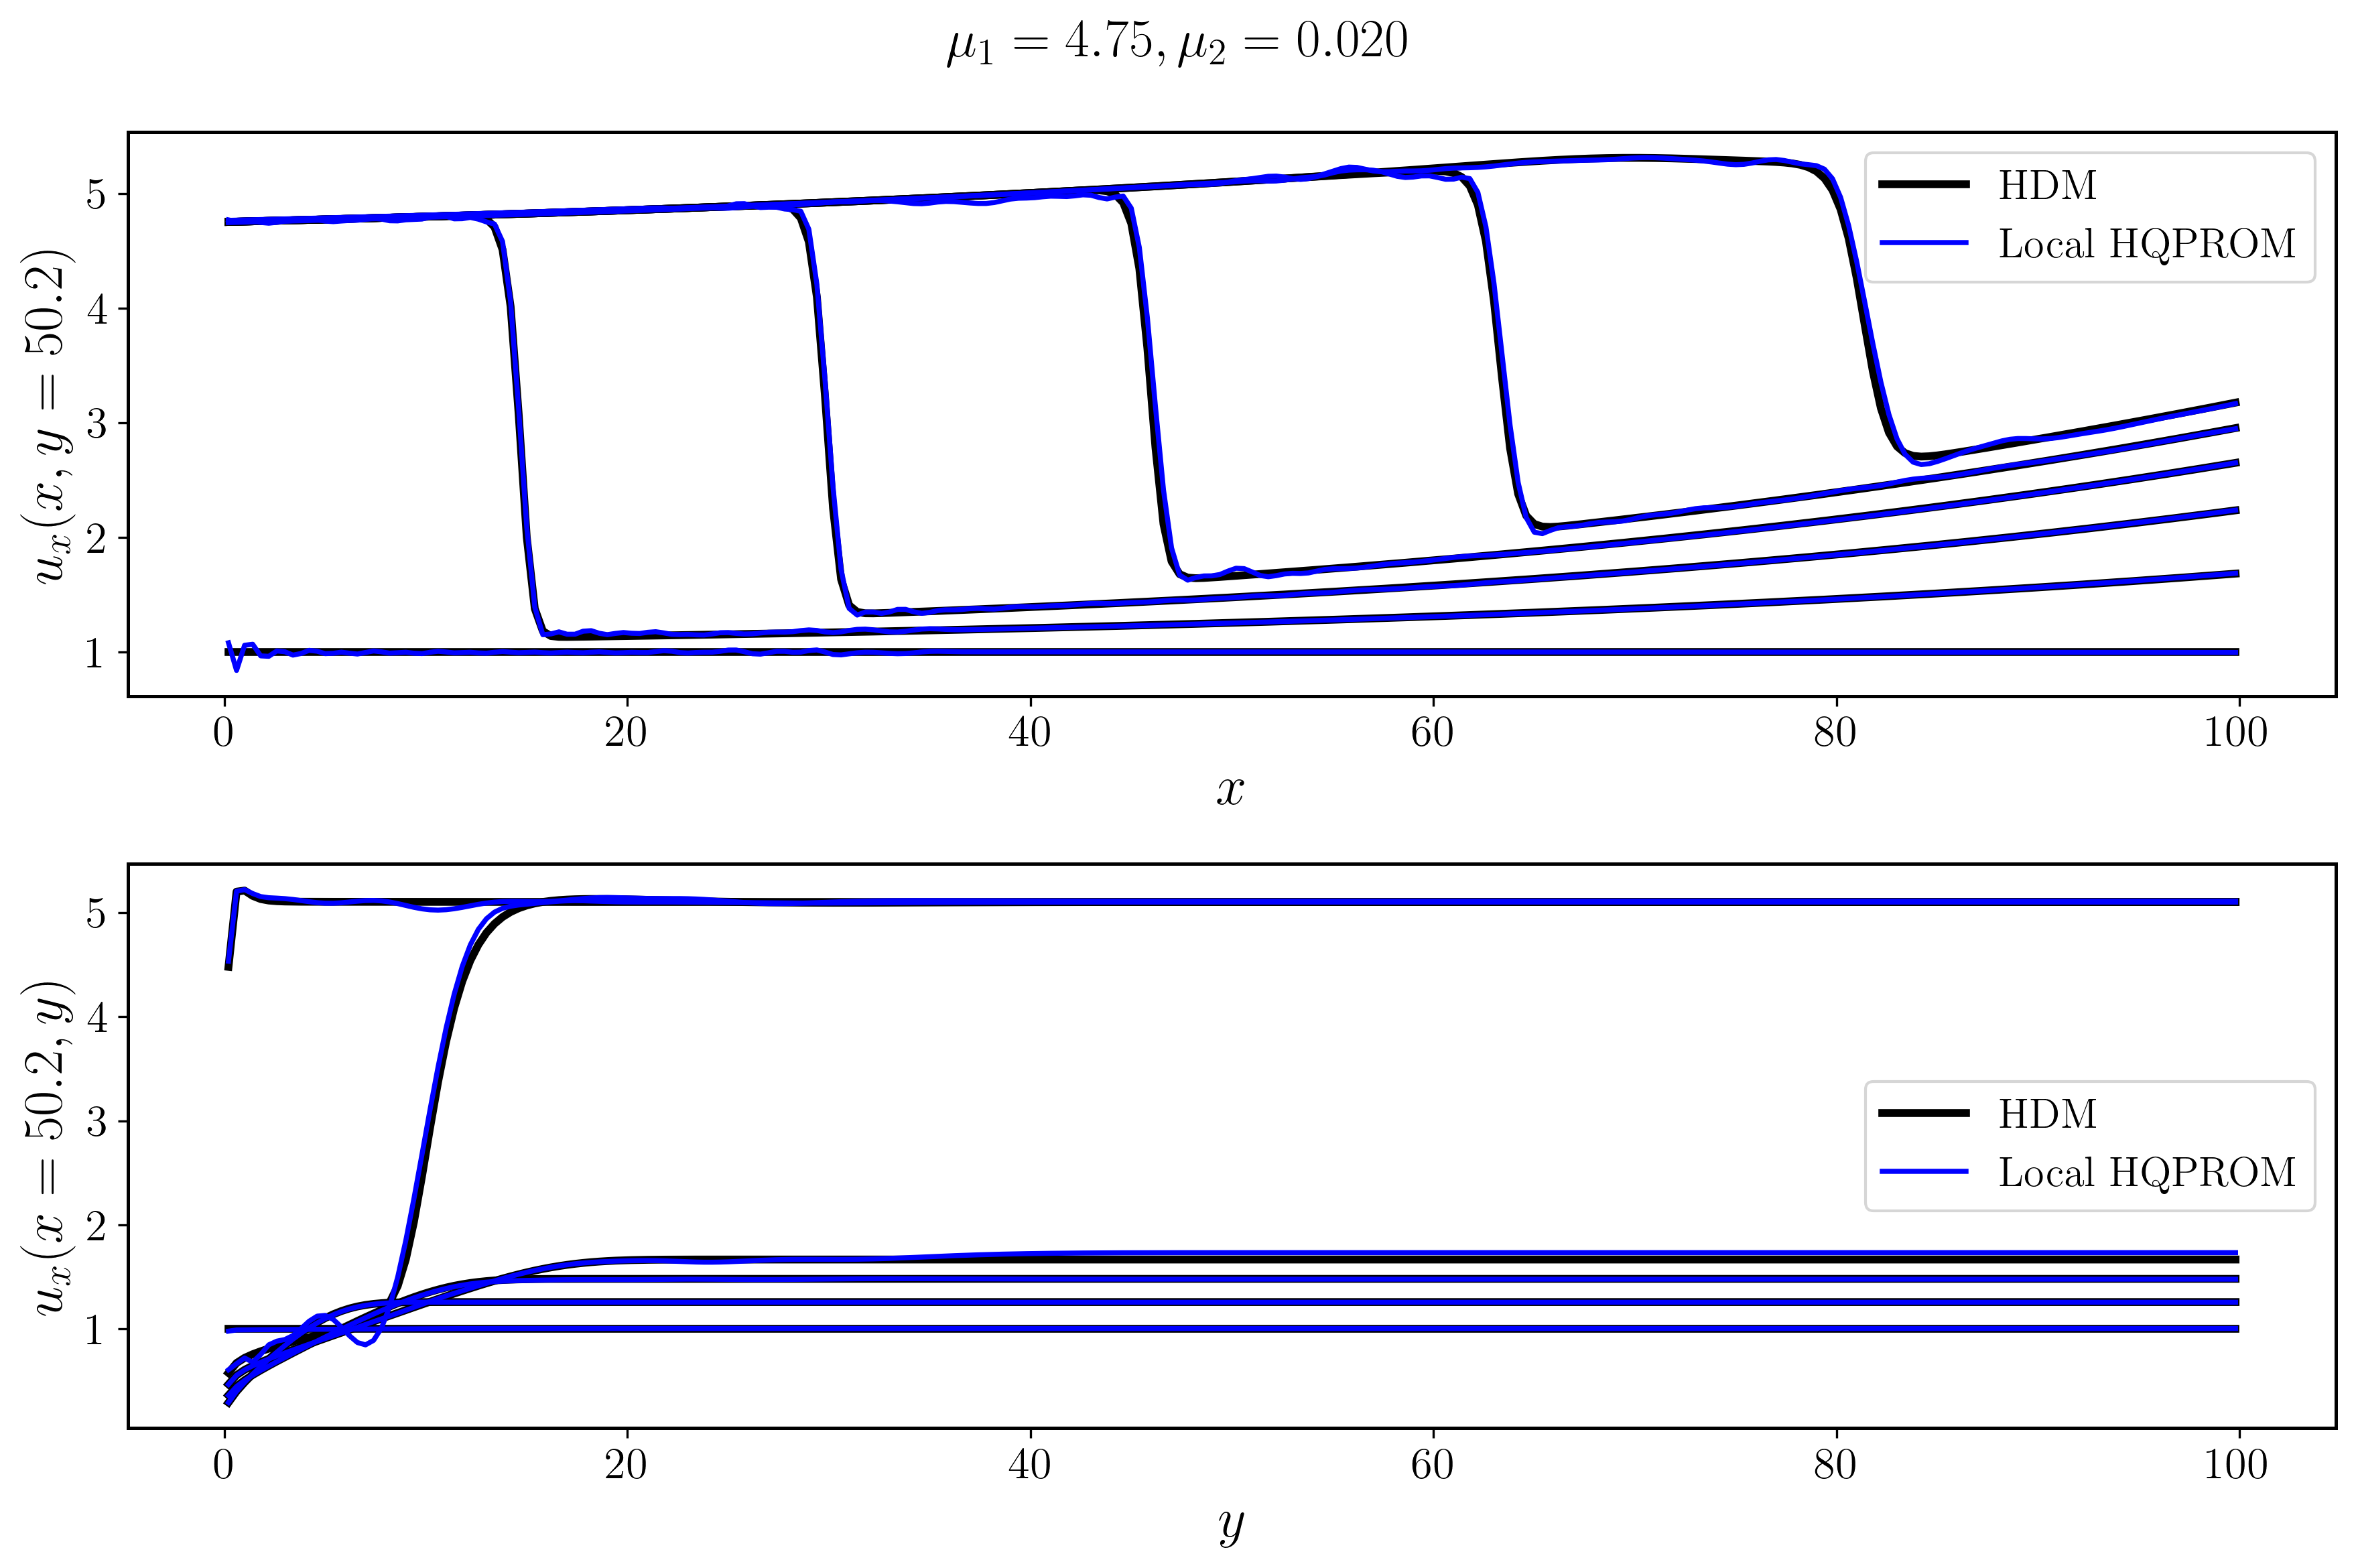
\includegraphics[width=0.82\textwidth,height=0.70\textheight,keepaspectratio]{Figures/local_hqprom_vs_hdm_mu1_4.75_mu2_0.020.png}
\end{frame}

\begin{frame}{Local HQPROM ($N_c=3$) vs HDM: $\boldsymbol\mu=(5.19,\,0.026)$}
\centering
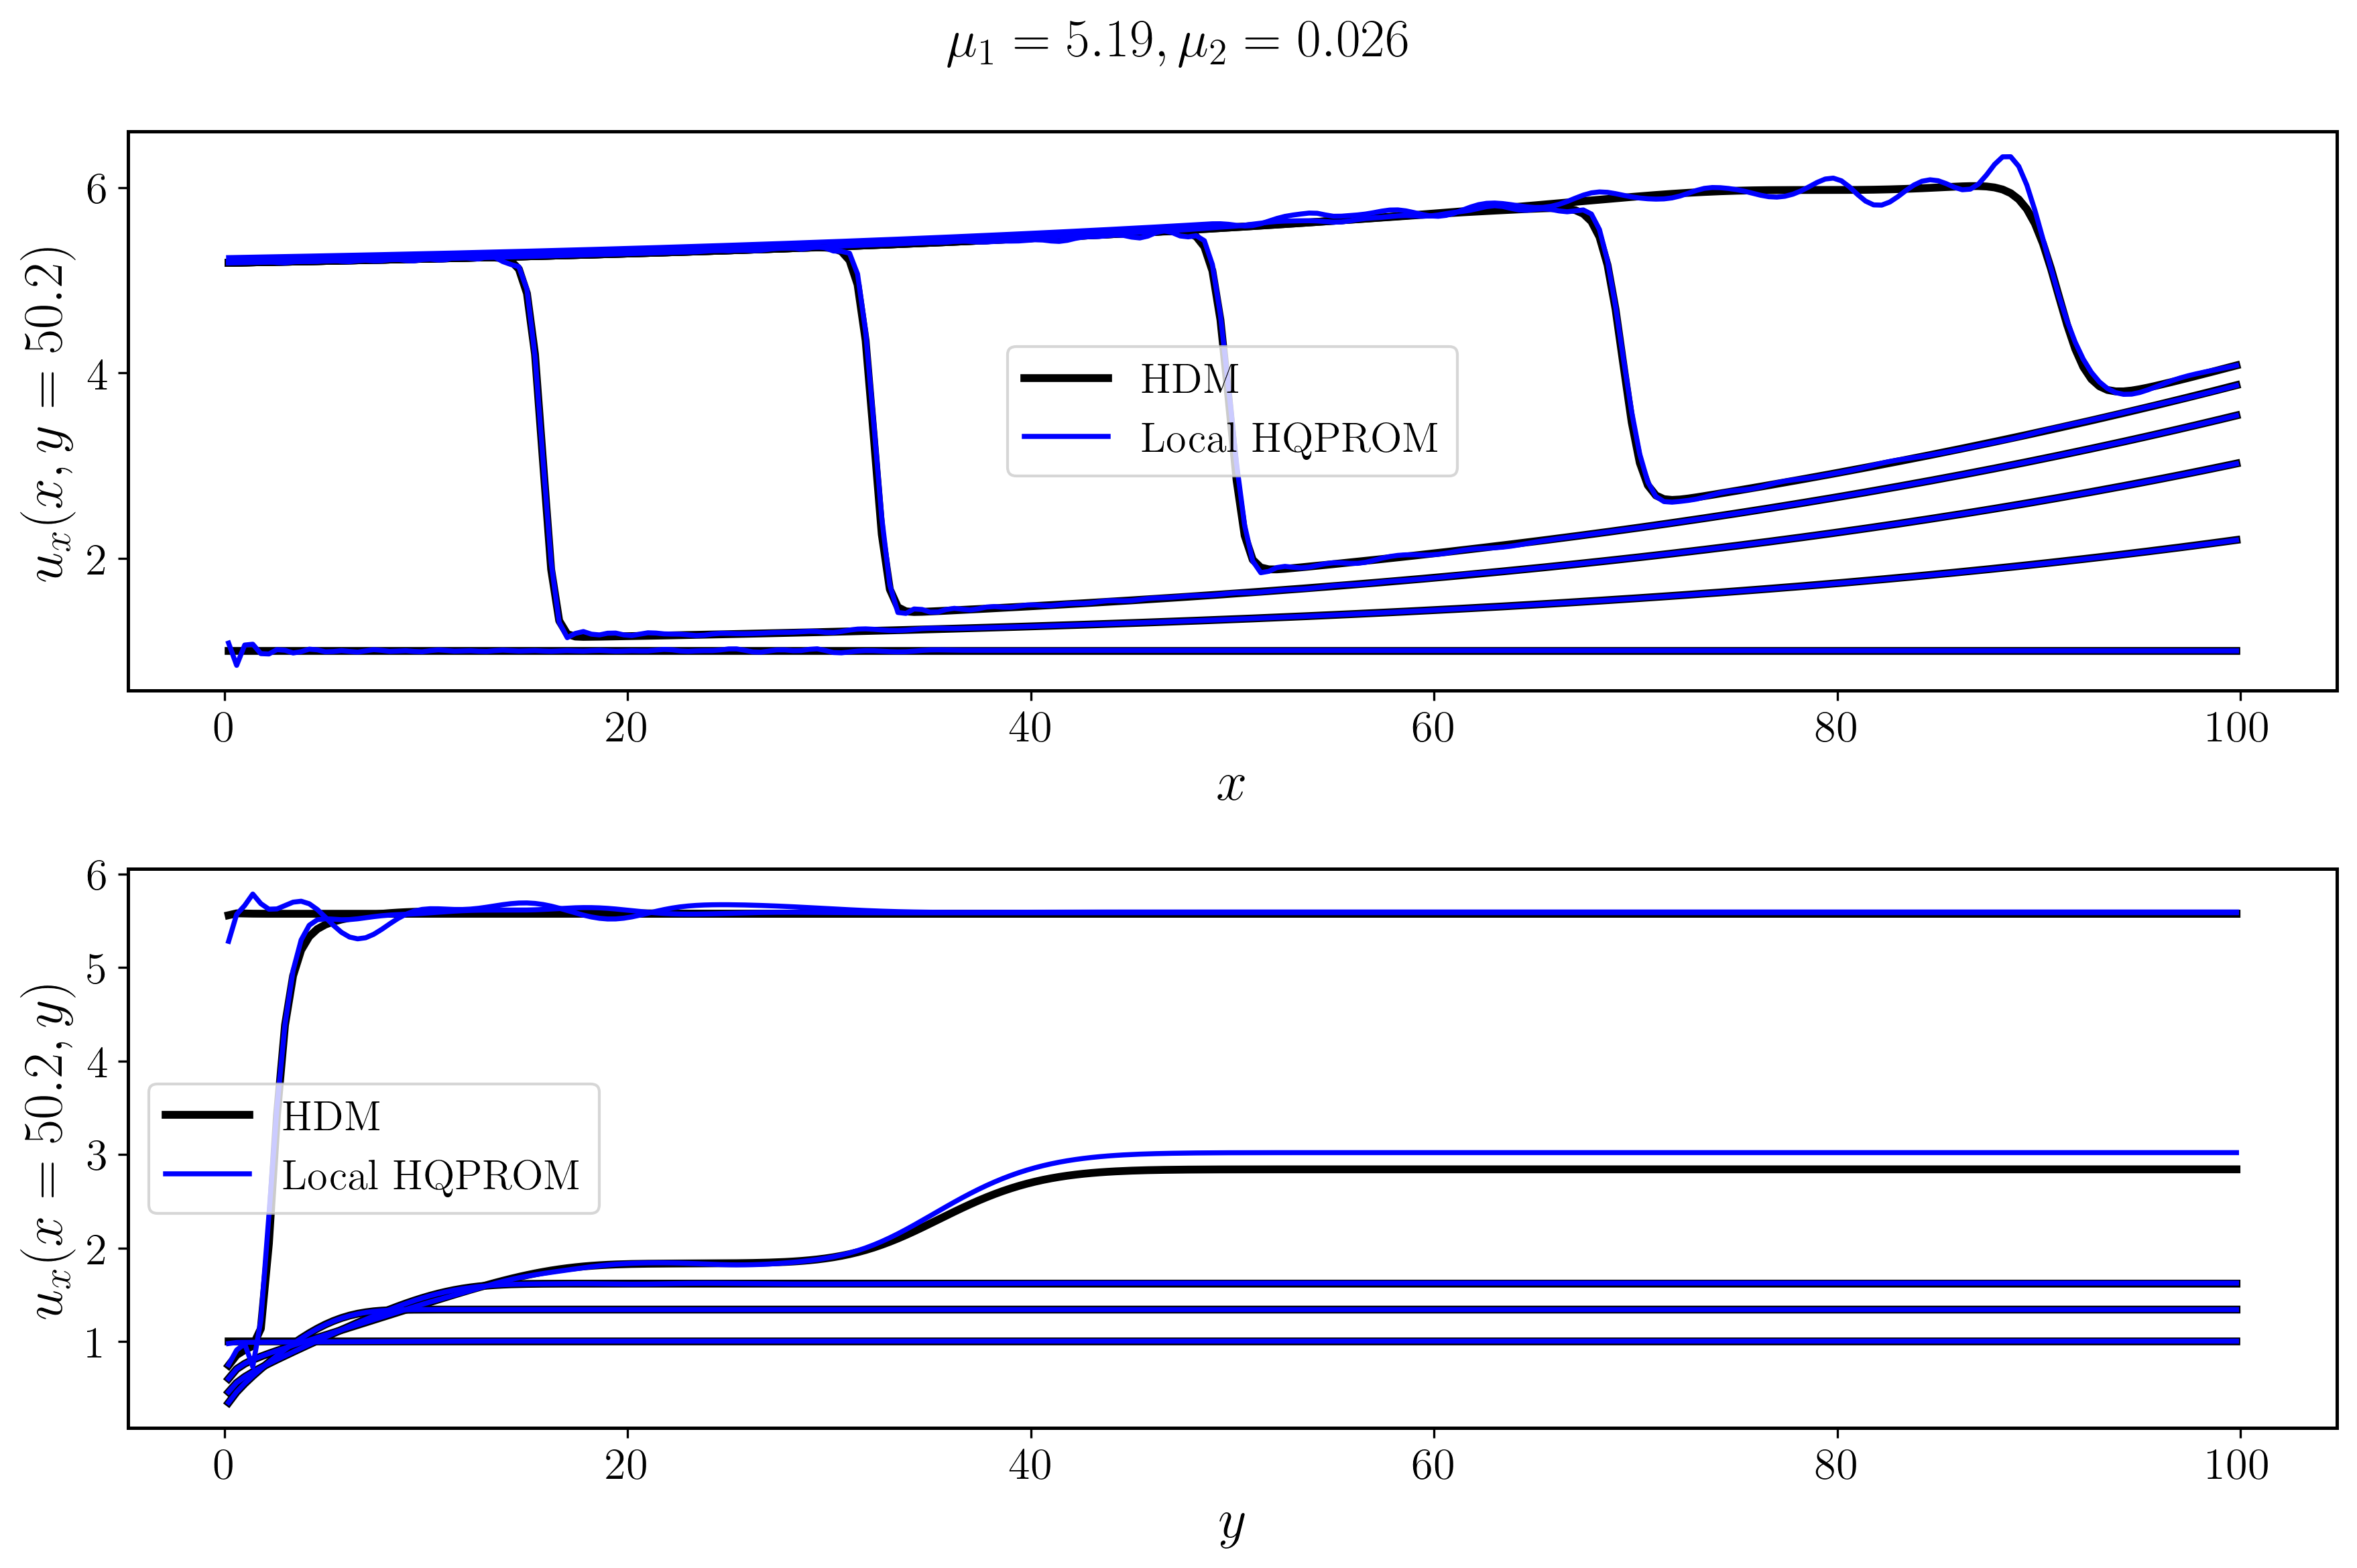
\includegraphics[width=0.82\textwidth,height=0.70\textheight,keepaspectratio]{Figures/local_hqprom_vs_hdm_mu1_5.19_mu2_0.026.png}
\end{frame}

\begin{frame}{HPROM-GPR vs HDM: $\boldsymbol\mu=(4.56,\,0.019)$}
\centering
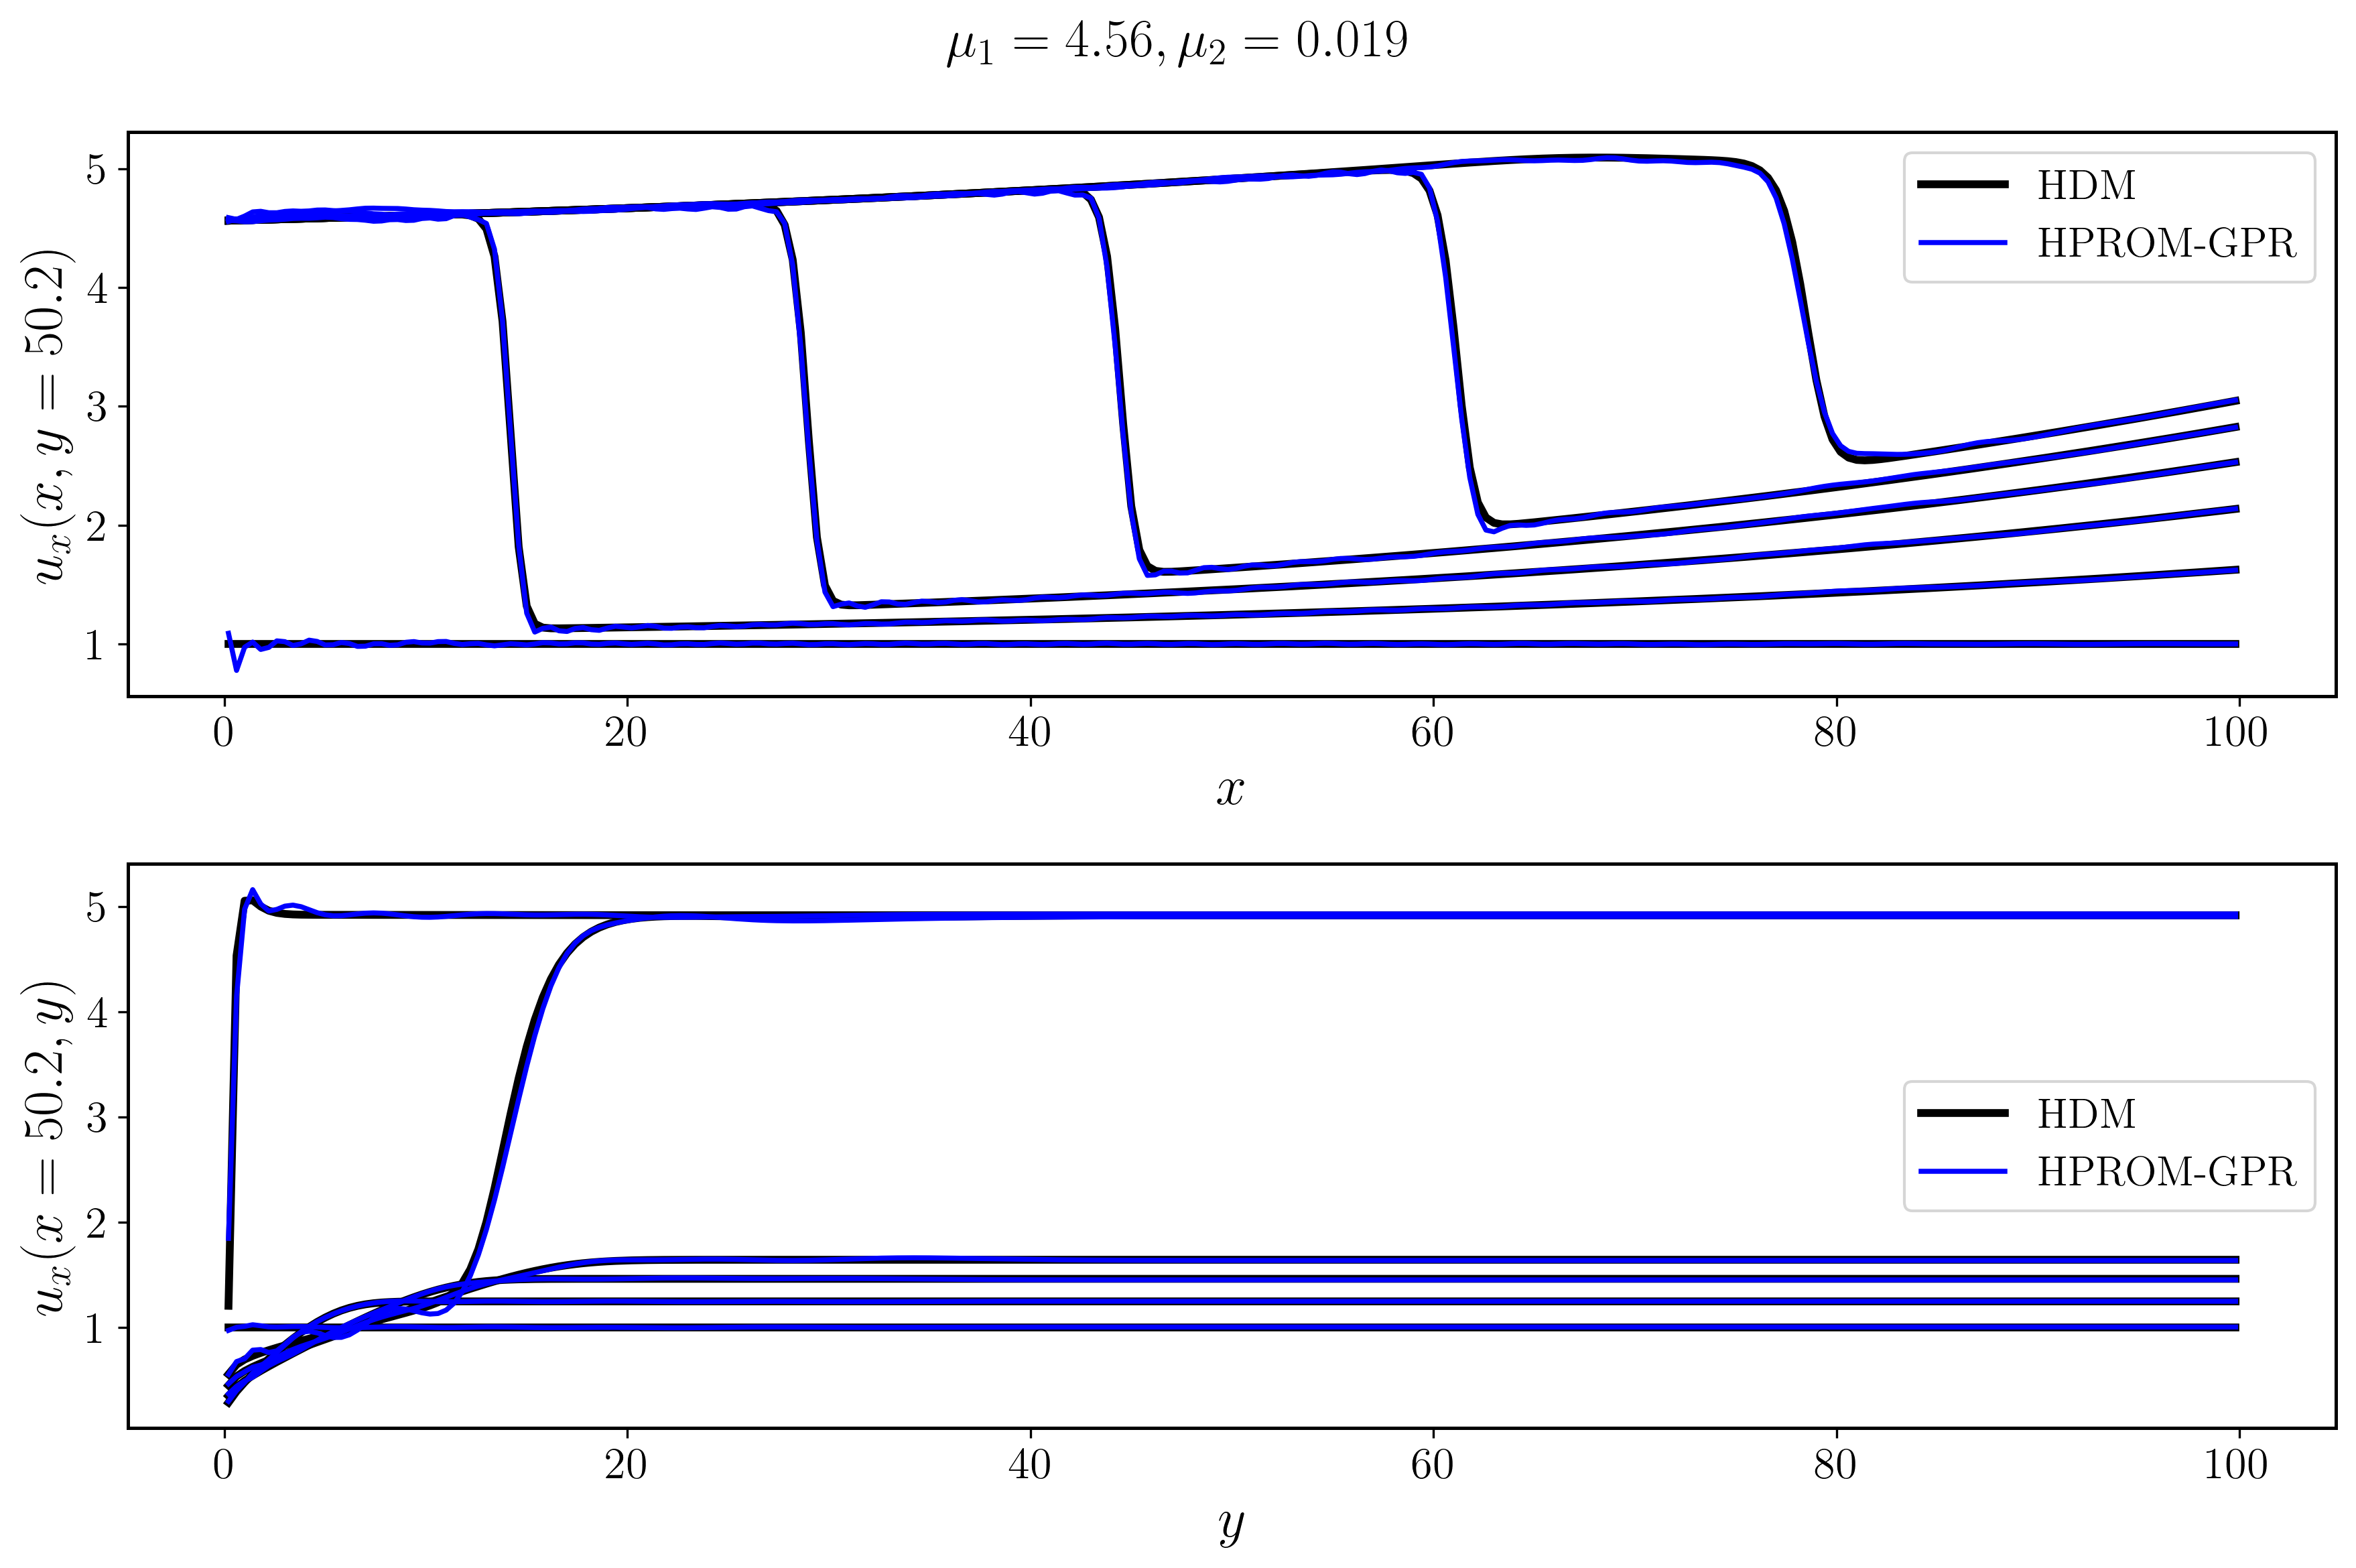
\includegraphics[width=0.82\textwidth,height=0.70\textheight,keepaspectratio]{Figures/hprom_gpr_vs_hdm_mu1_4.56_mu2_0.019.png}
\end{frame}

\begin{frame}{HPROM-GPR vs HDM: $\boldsymbol\mu=(4.75,\,0.020)$}
\centering
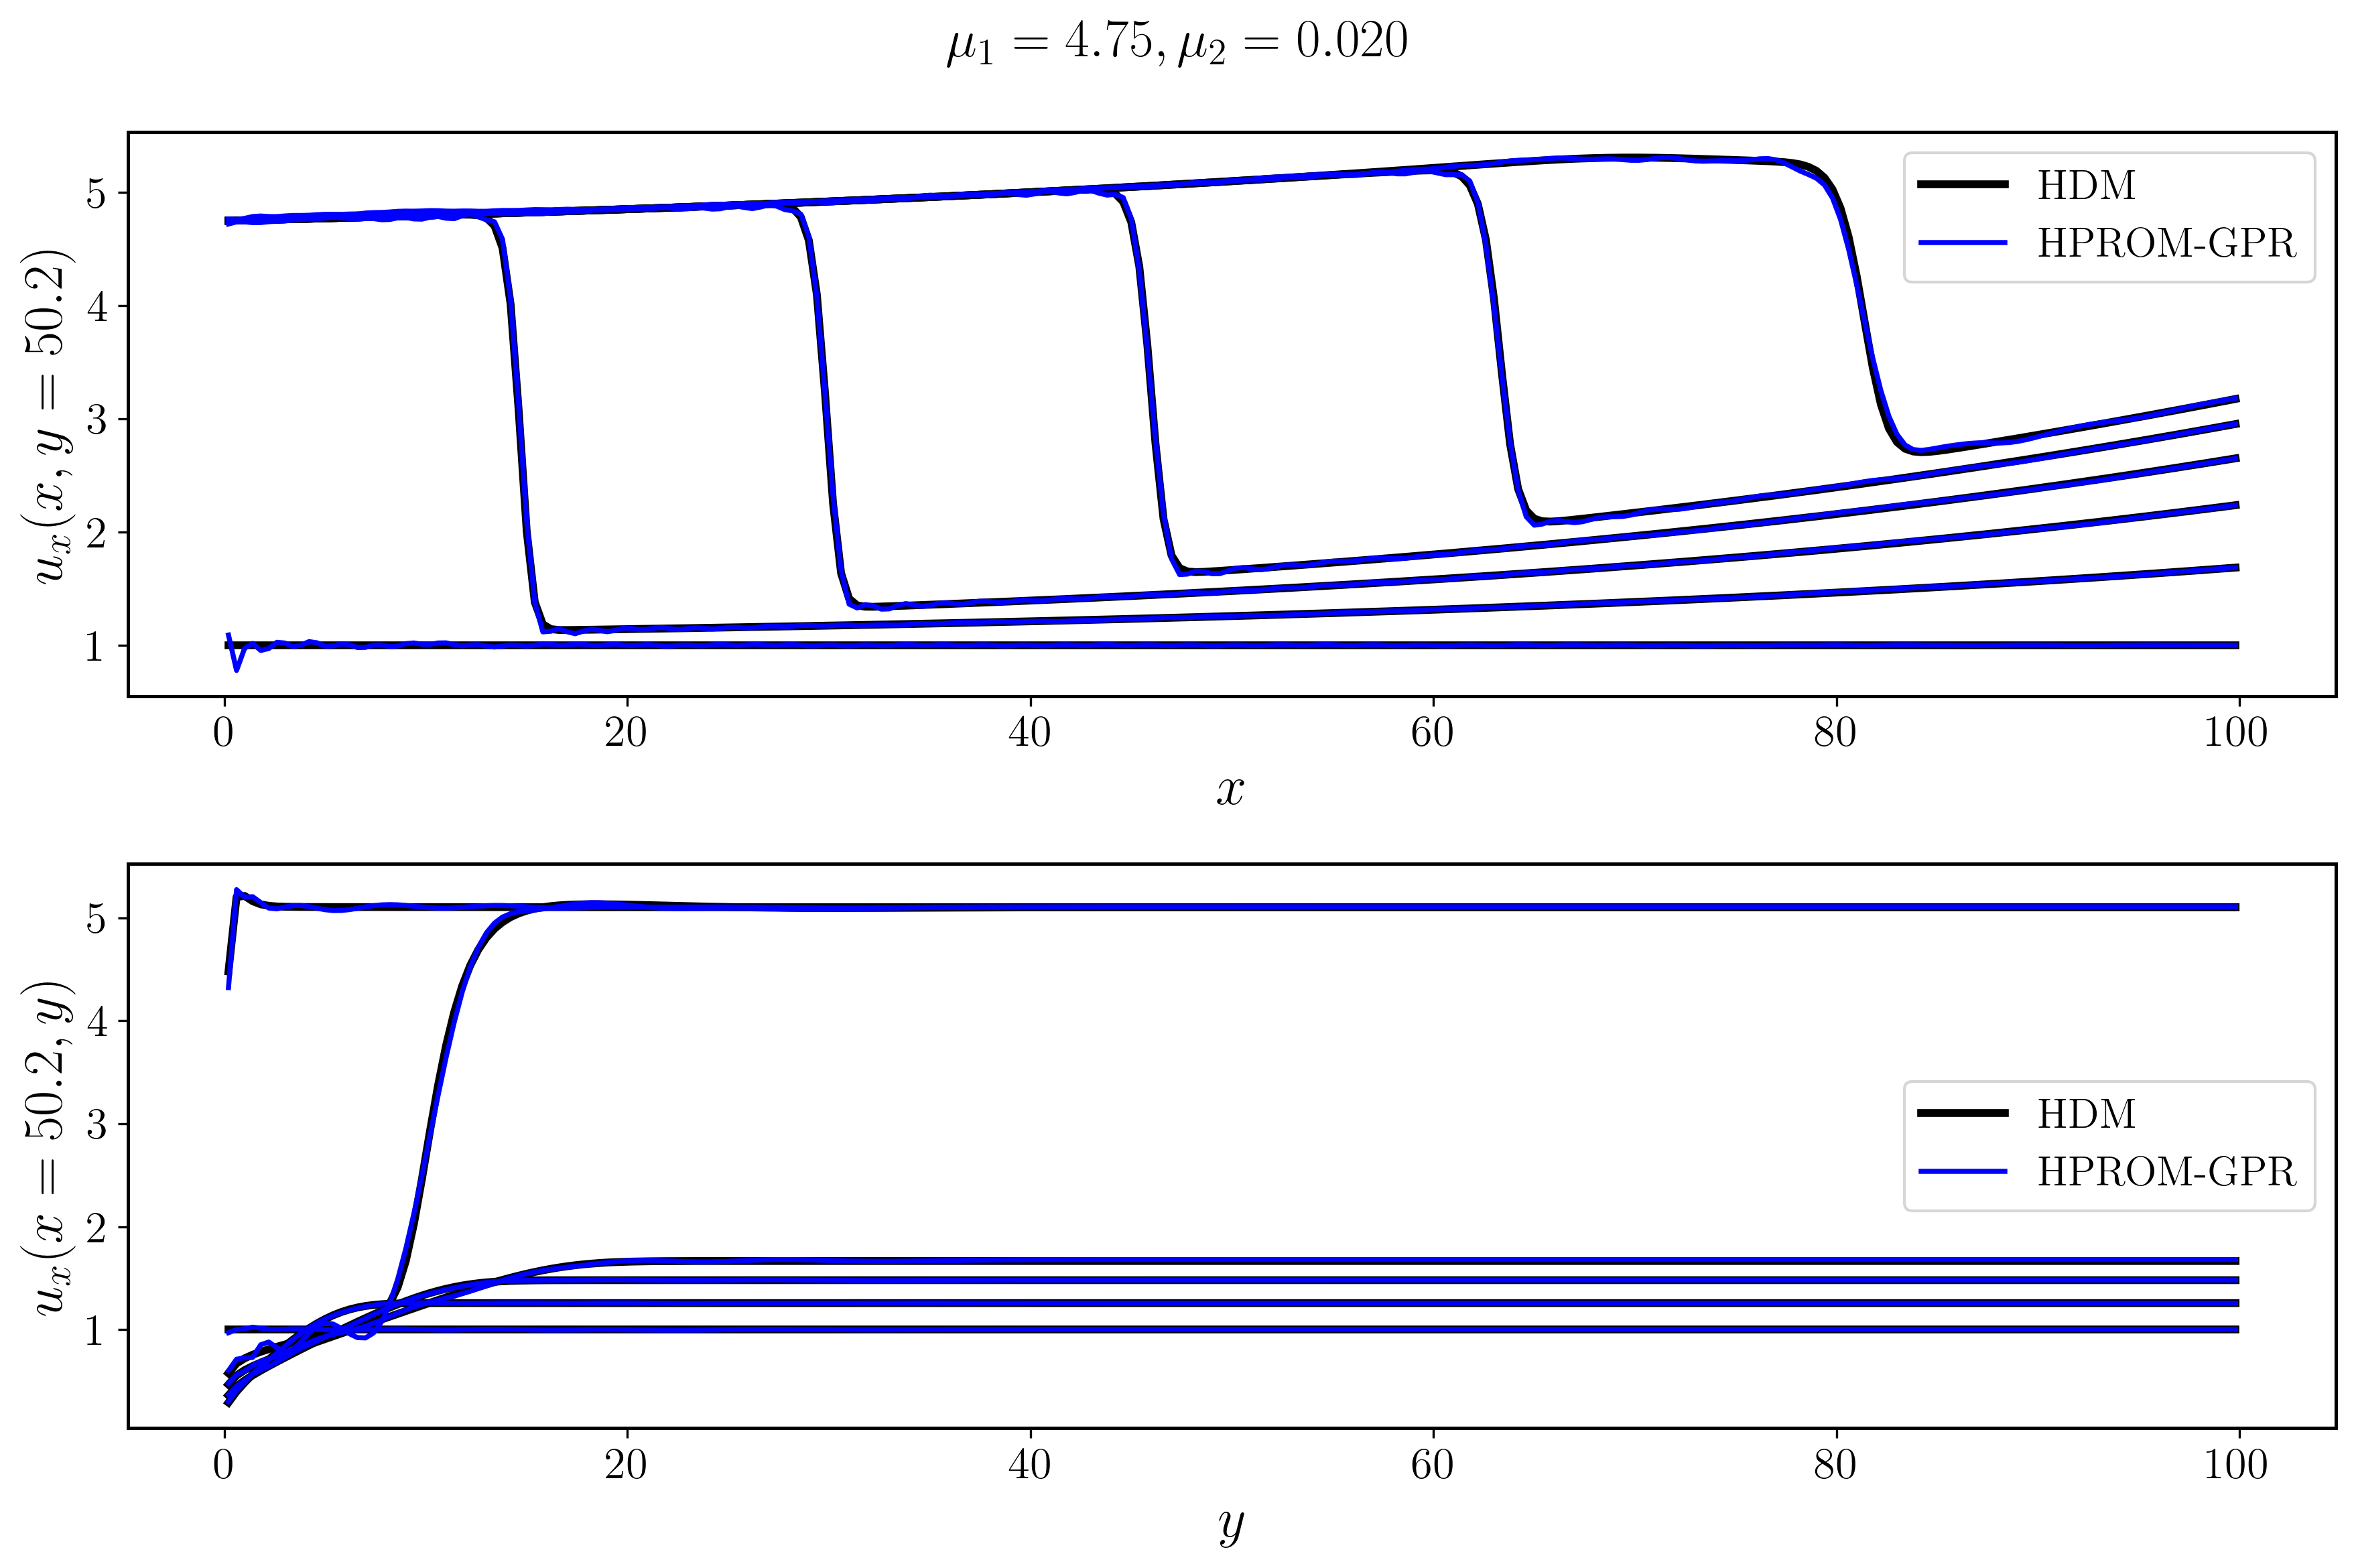
\includegraphics[width=0.82\textwidth,height=0.70\textheight,keepaspectratio]{Figures/hprom_gpr_vs_hdm_mu1_4.75_mu2_0.020.png}
\end{frame}

\begin{frame}{HPROM-GPR vs HDM: $\boldsymbol\mu=(5.19,\,0.026)$}
\centering
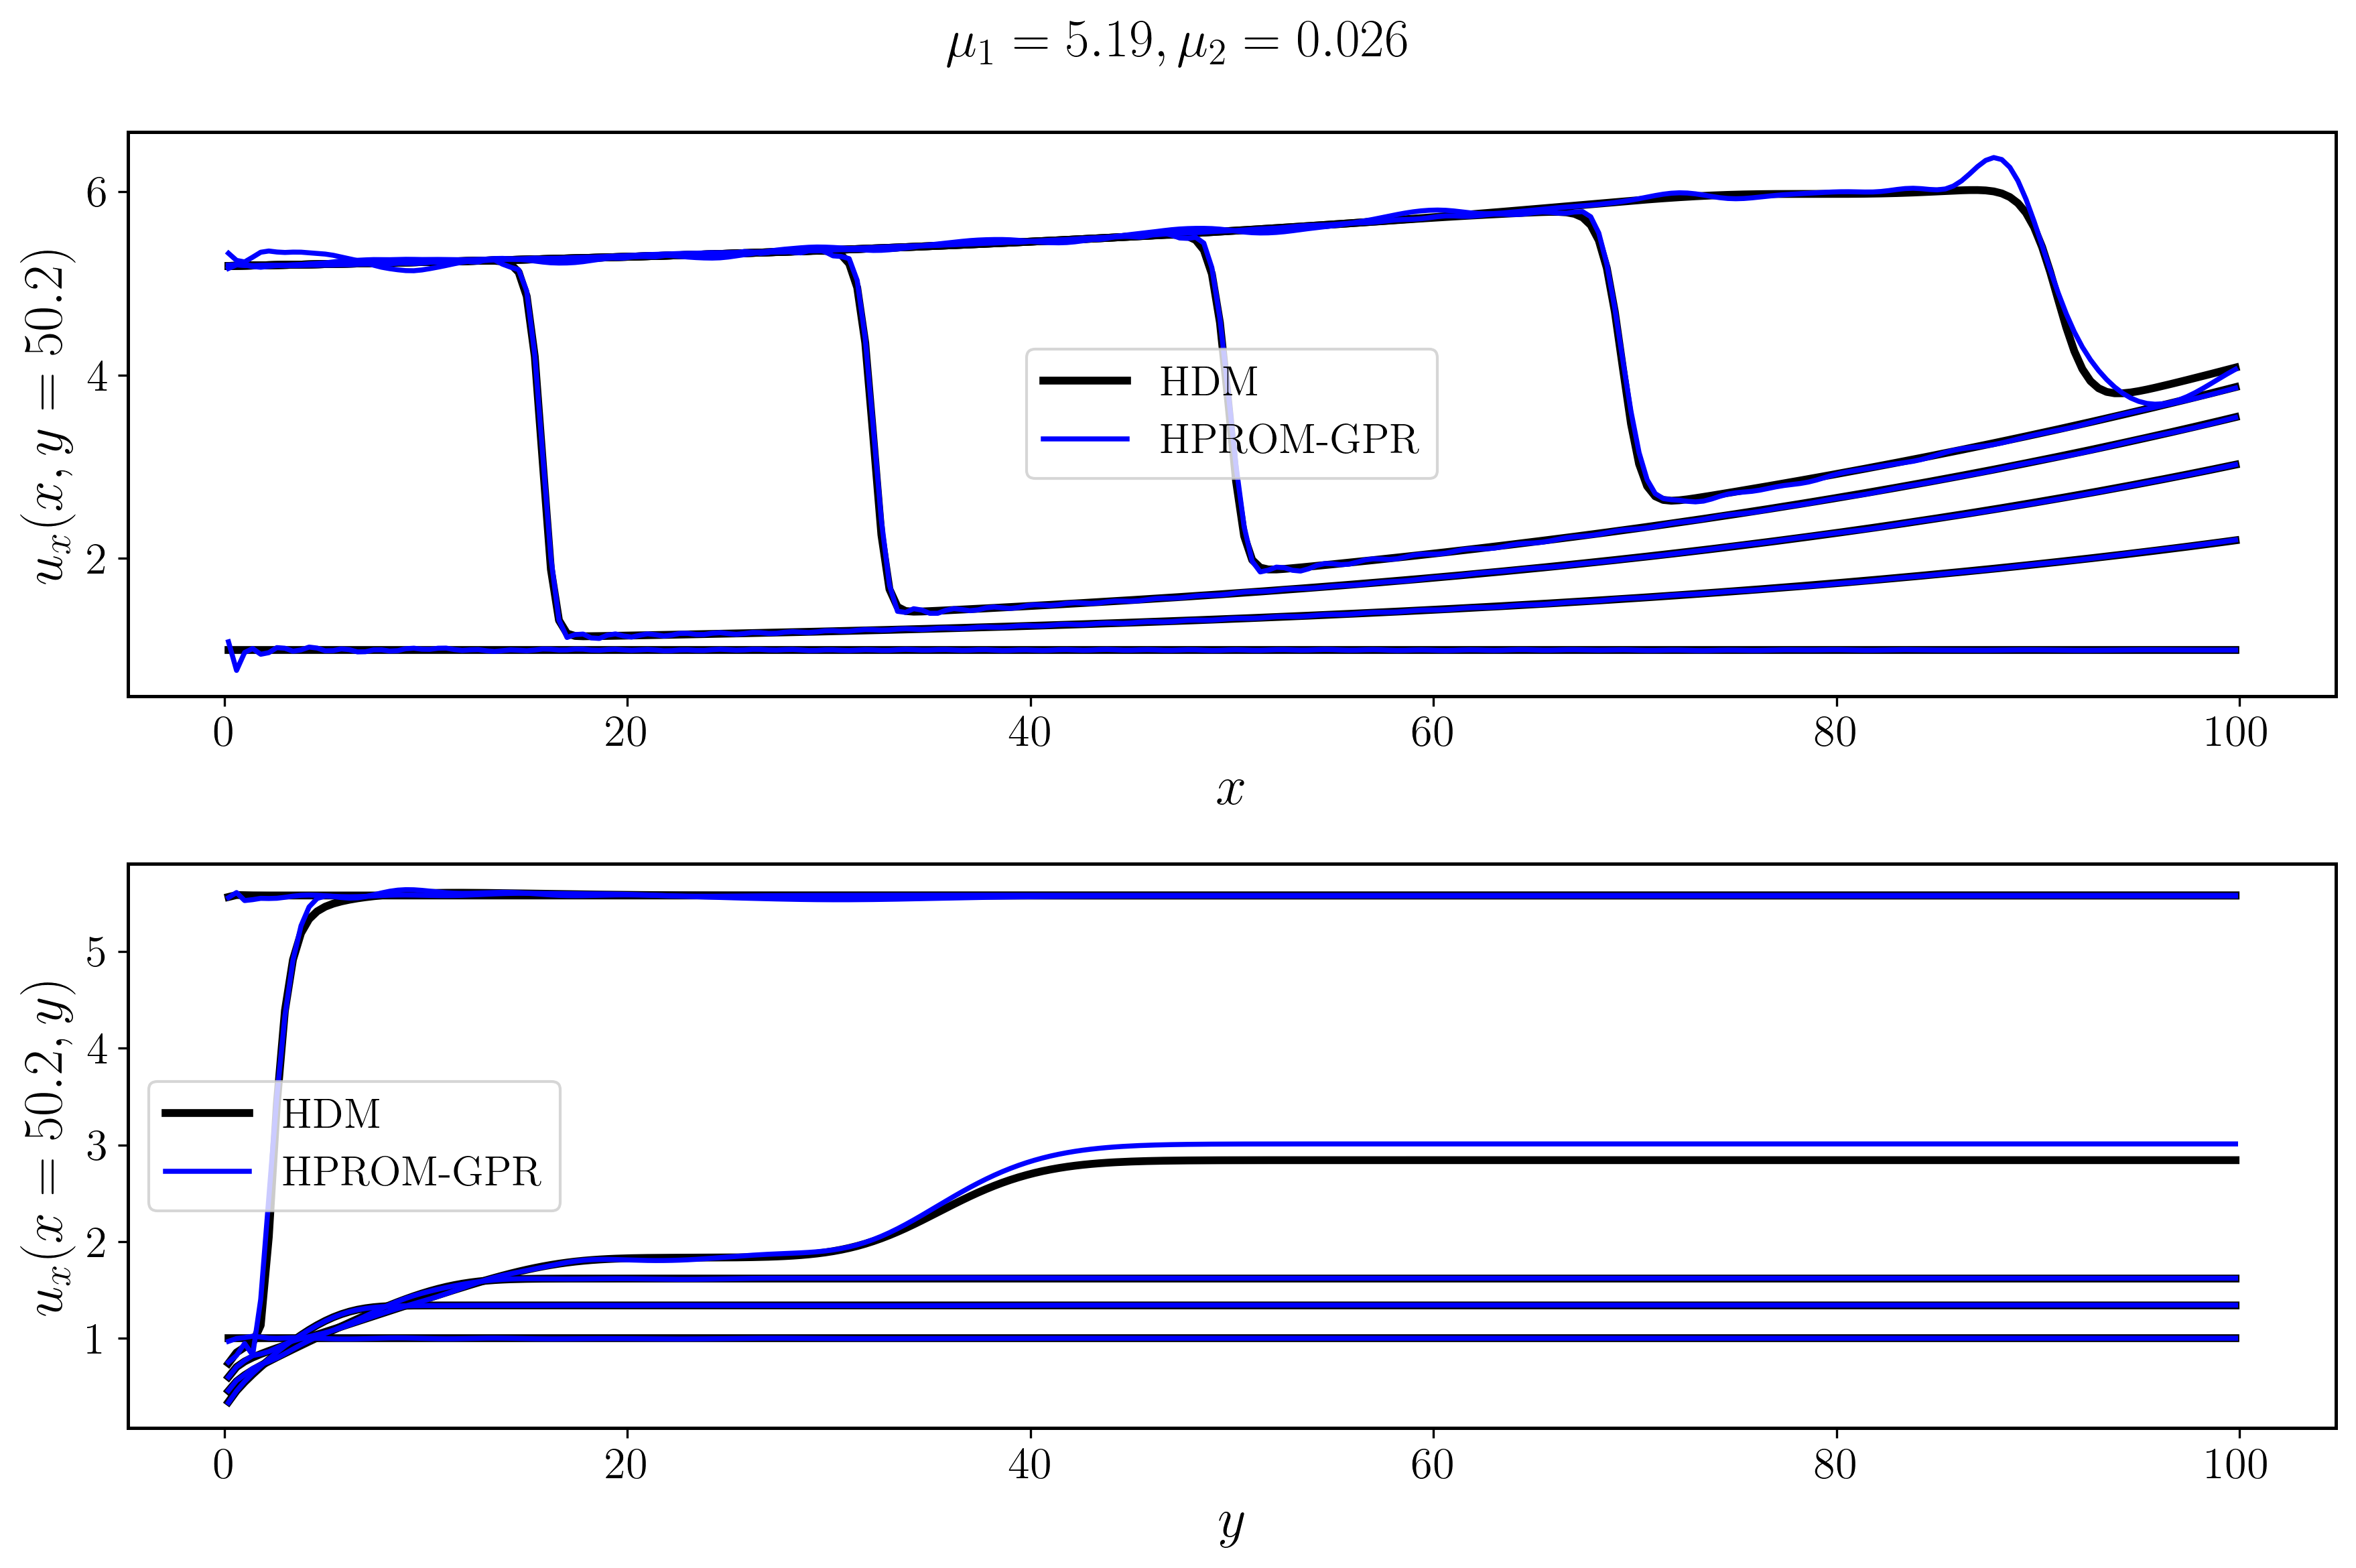
\includegraphics[width=0.82\textwidth,height=0.70\textheight,keepaspectratio]{Figures/hprom_gpr_vs_hdm_mu1_5.19_mu2_0.026.png}
\end{frame}

\begin{frame}{Local HPROM-GPR ($N_c=3$) vs HDM: $\boldsymbol\mu=(4.56,\,0.019)$}
\centering
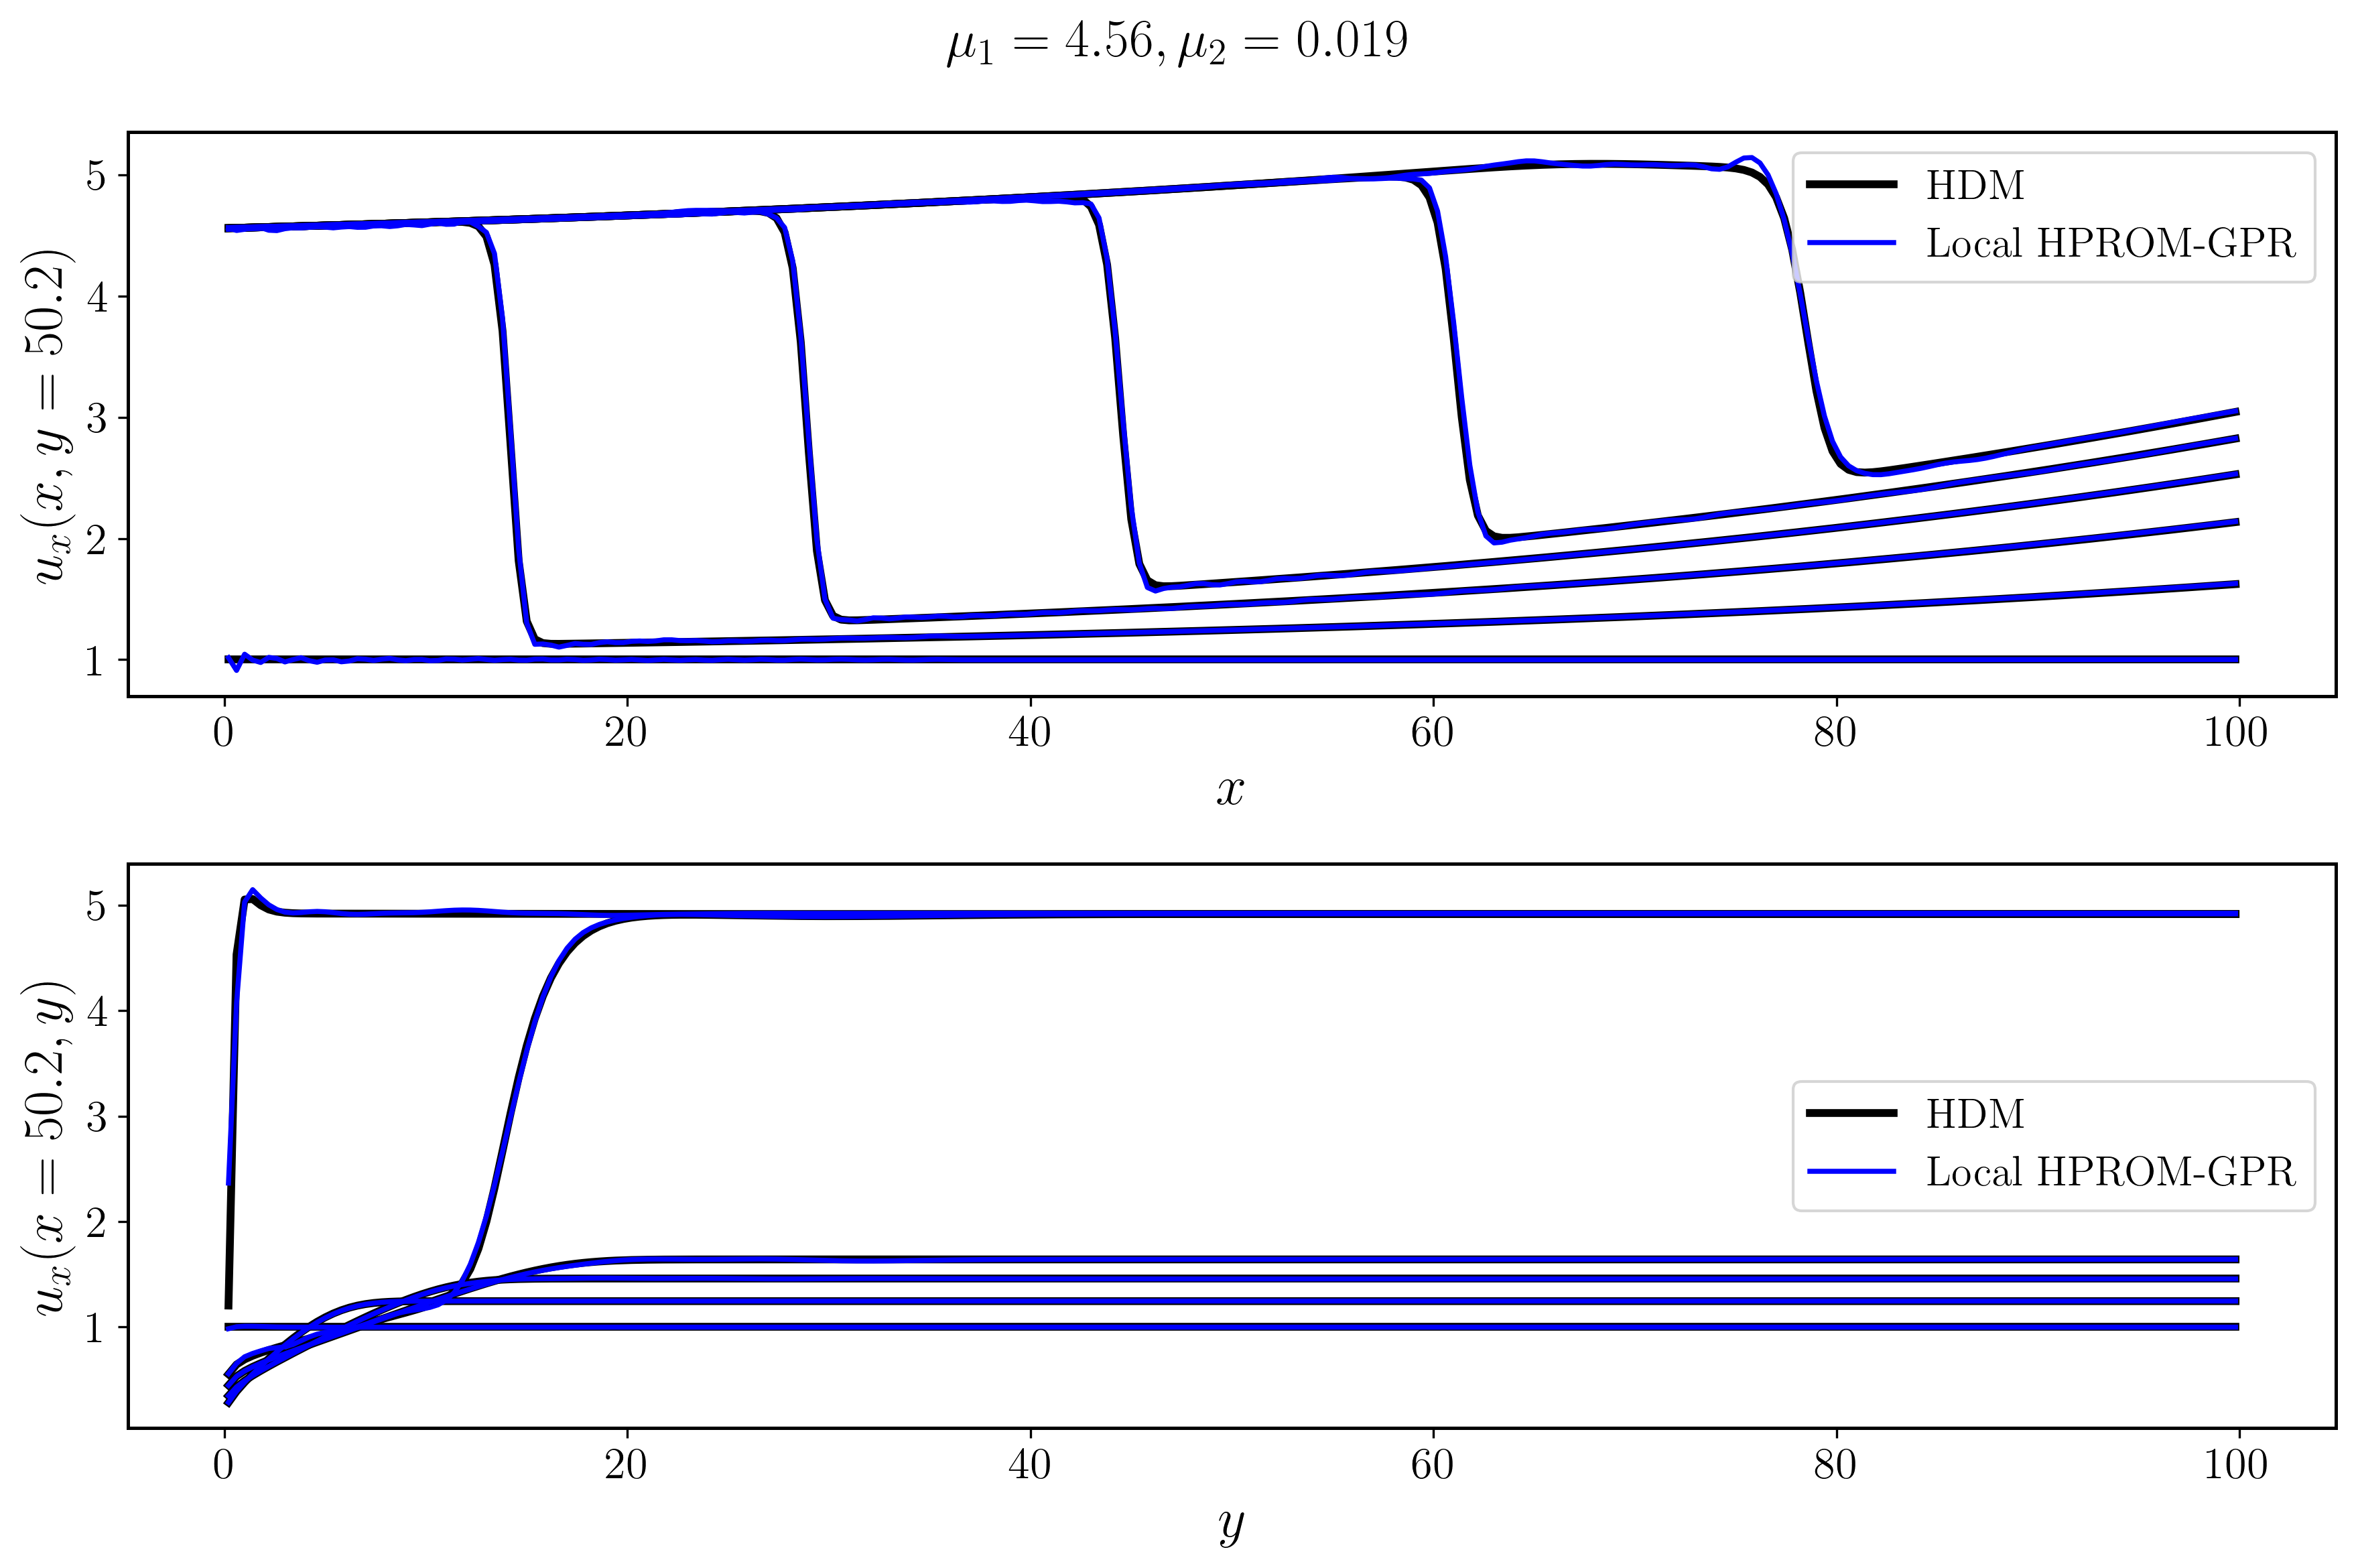
\includegraphics[width=0.82\textwidth,height=0.70\textheight,keepaspectratio]{Figures/local_hprom_gpr_vs_hdm_mu1_4.56_mu2_0.019.png}
\end{frame}

\begin{frame}{Local HPROM-GPR ($N_c=3$) vs HDM: $\boldsymbol\mu=(4.75,\,0.020)$}
\centering
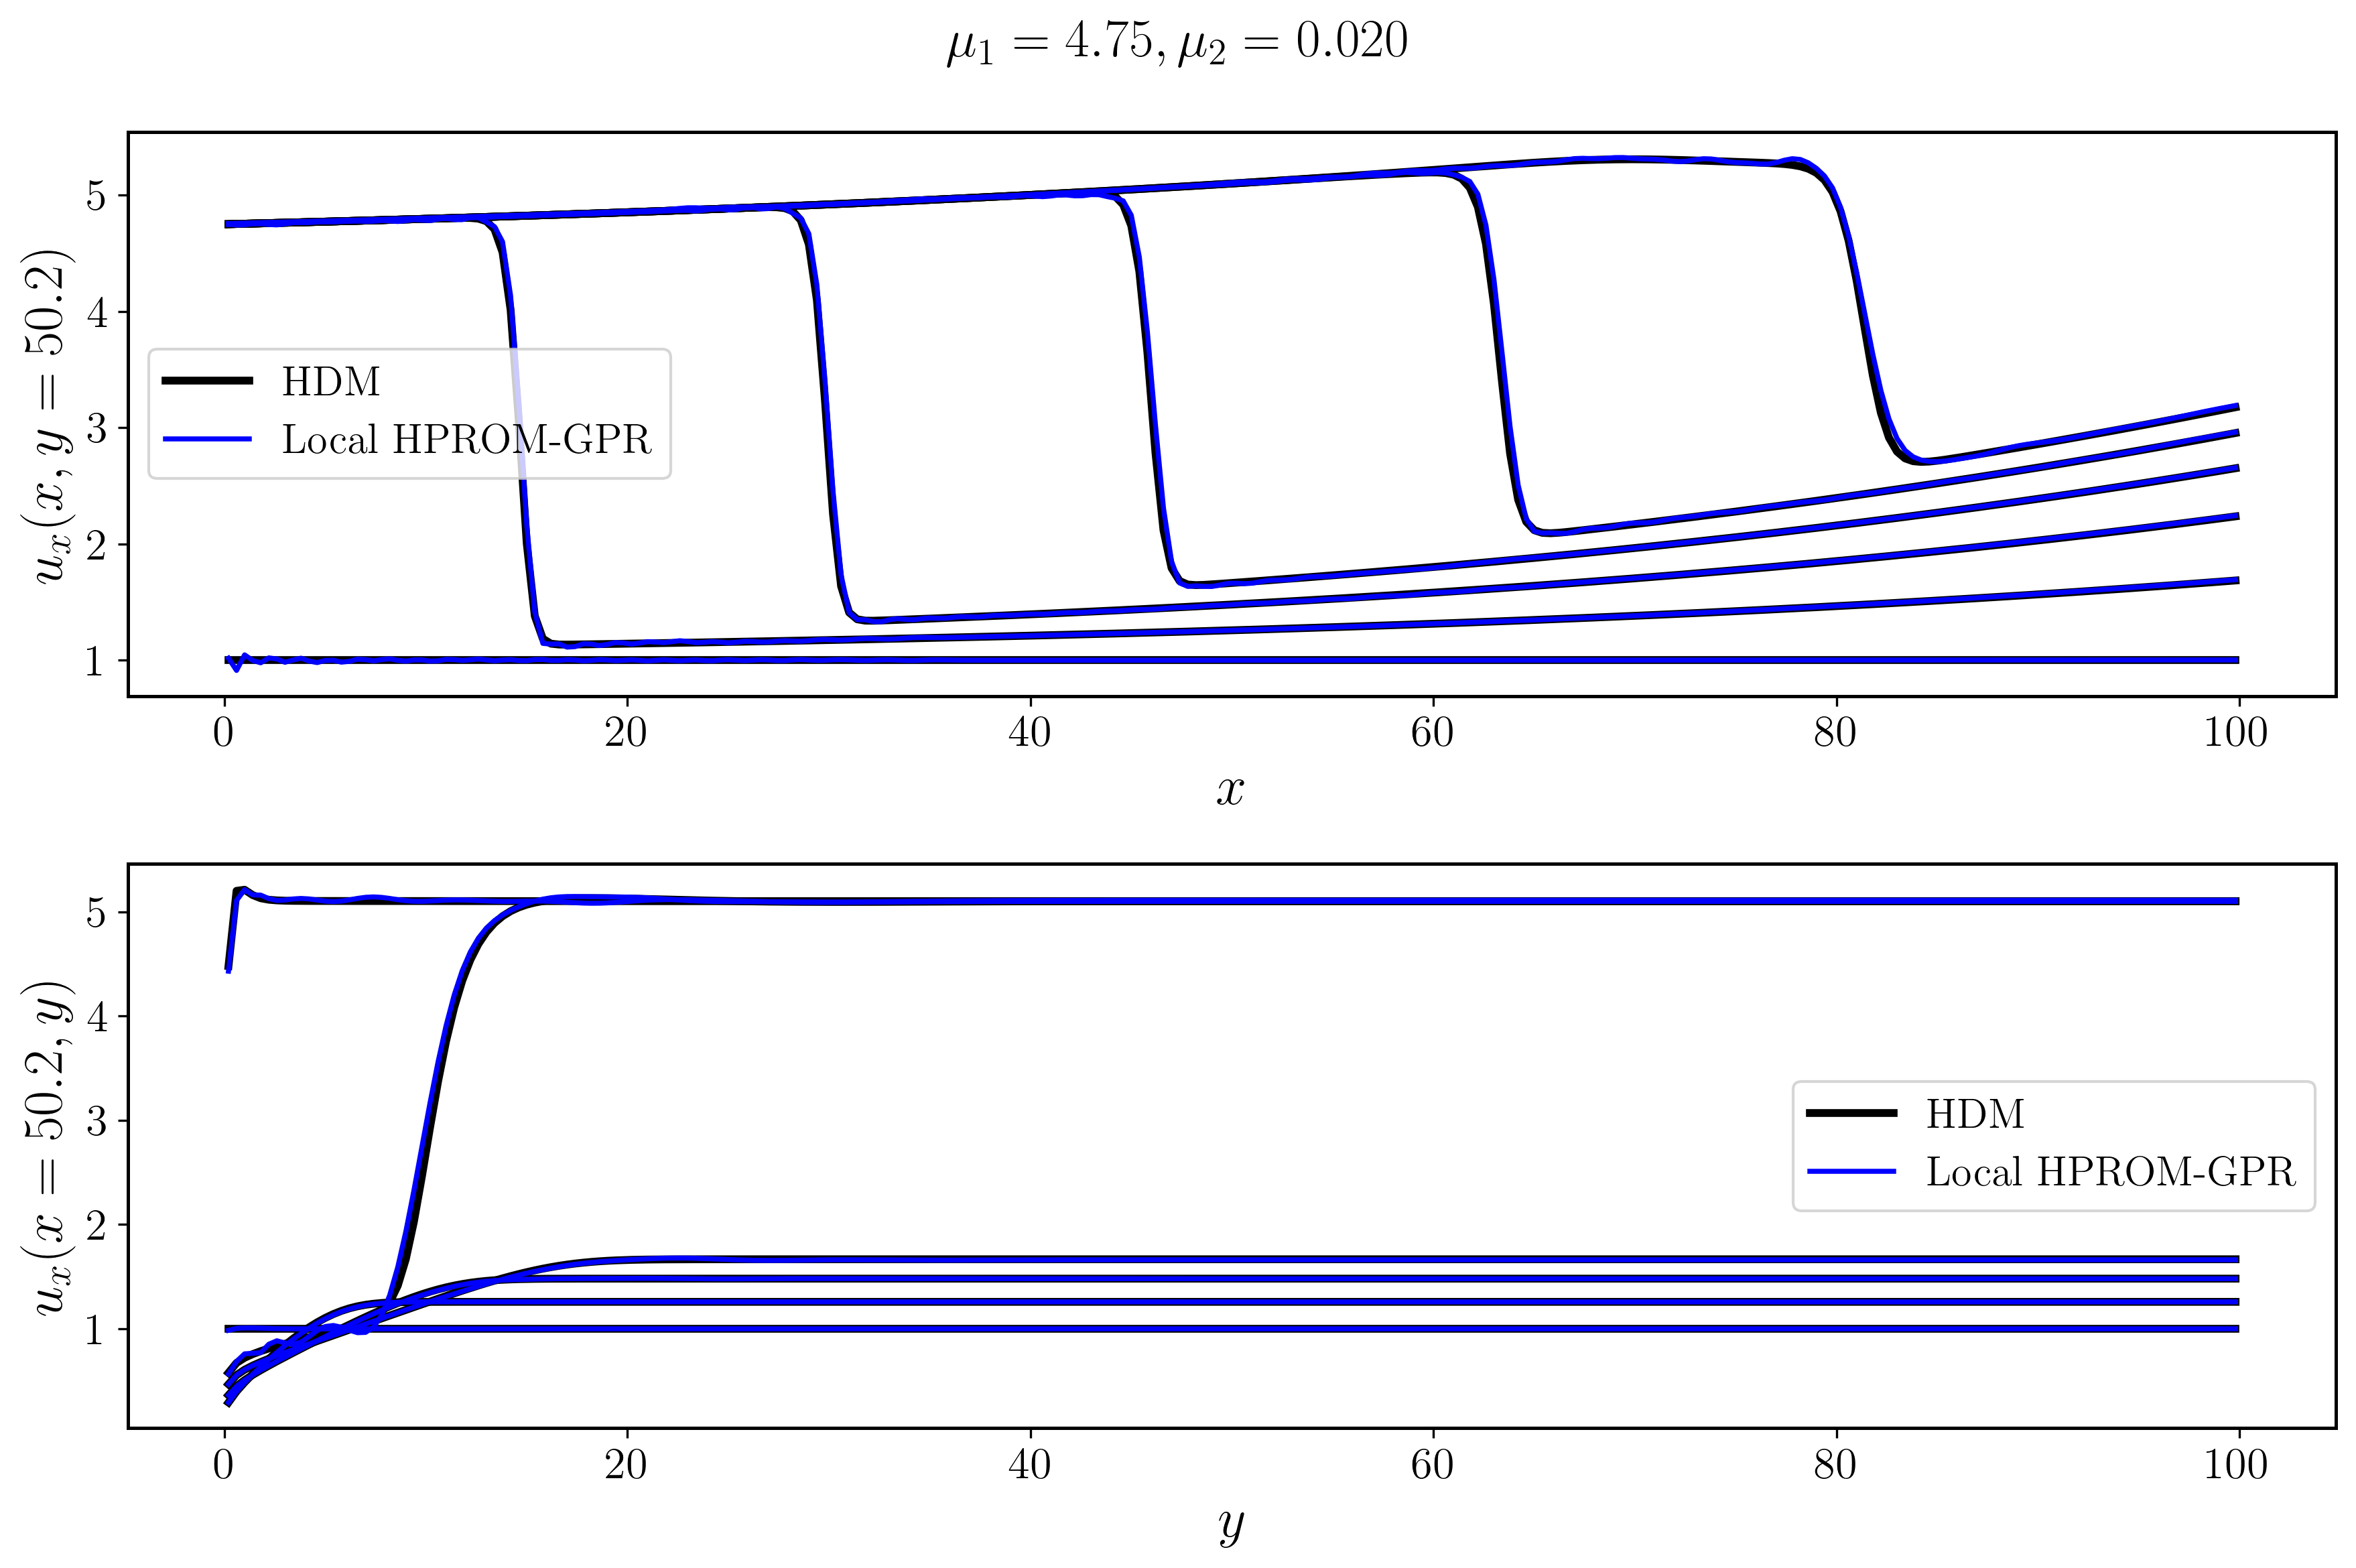
\includegraphics[width=0.82\textwidth,height=0.70\textheight,keepaspectratio]{Figures/local_hprom_gpr_vs_hdm_mu1_4.75_mu2_0.020.png}
\end{frame}

\begin{frame}{Local HPROM-GPR ($N_c=3$) vs HDM: $\boldsymbol\mu=(5.19,\,0.026)$}
\centering
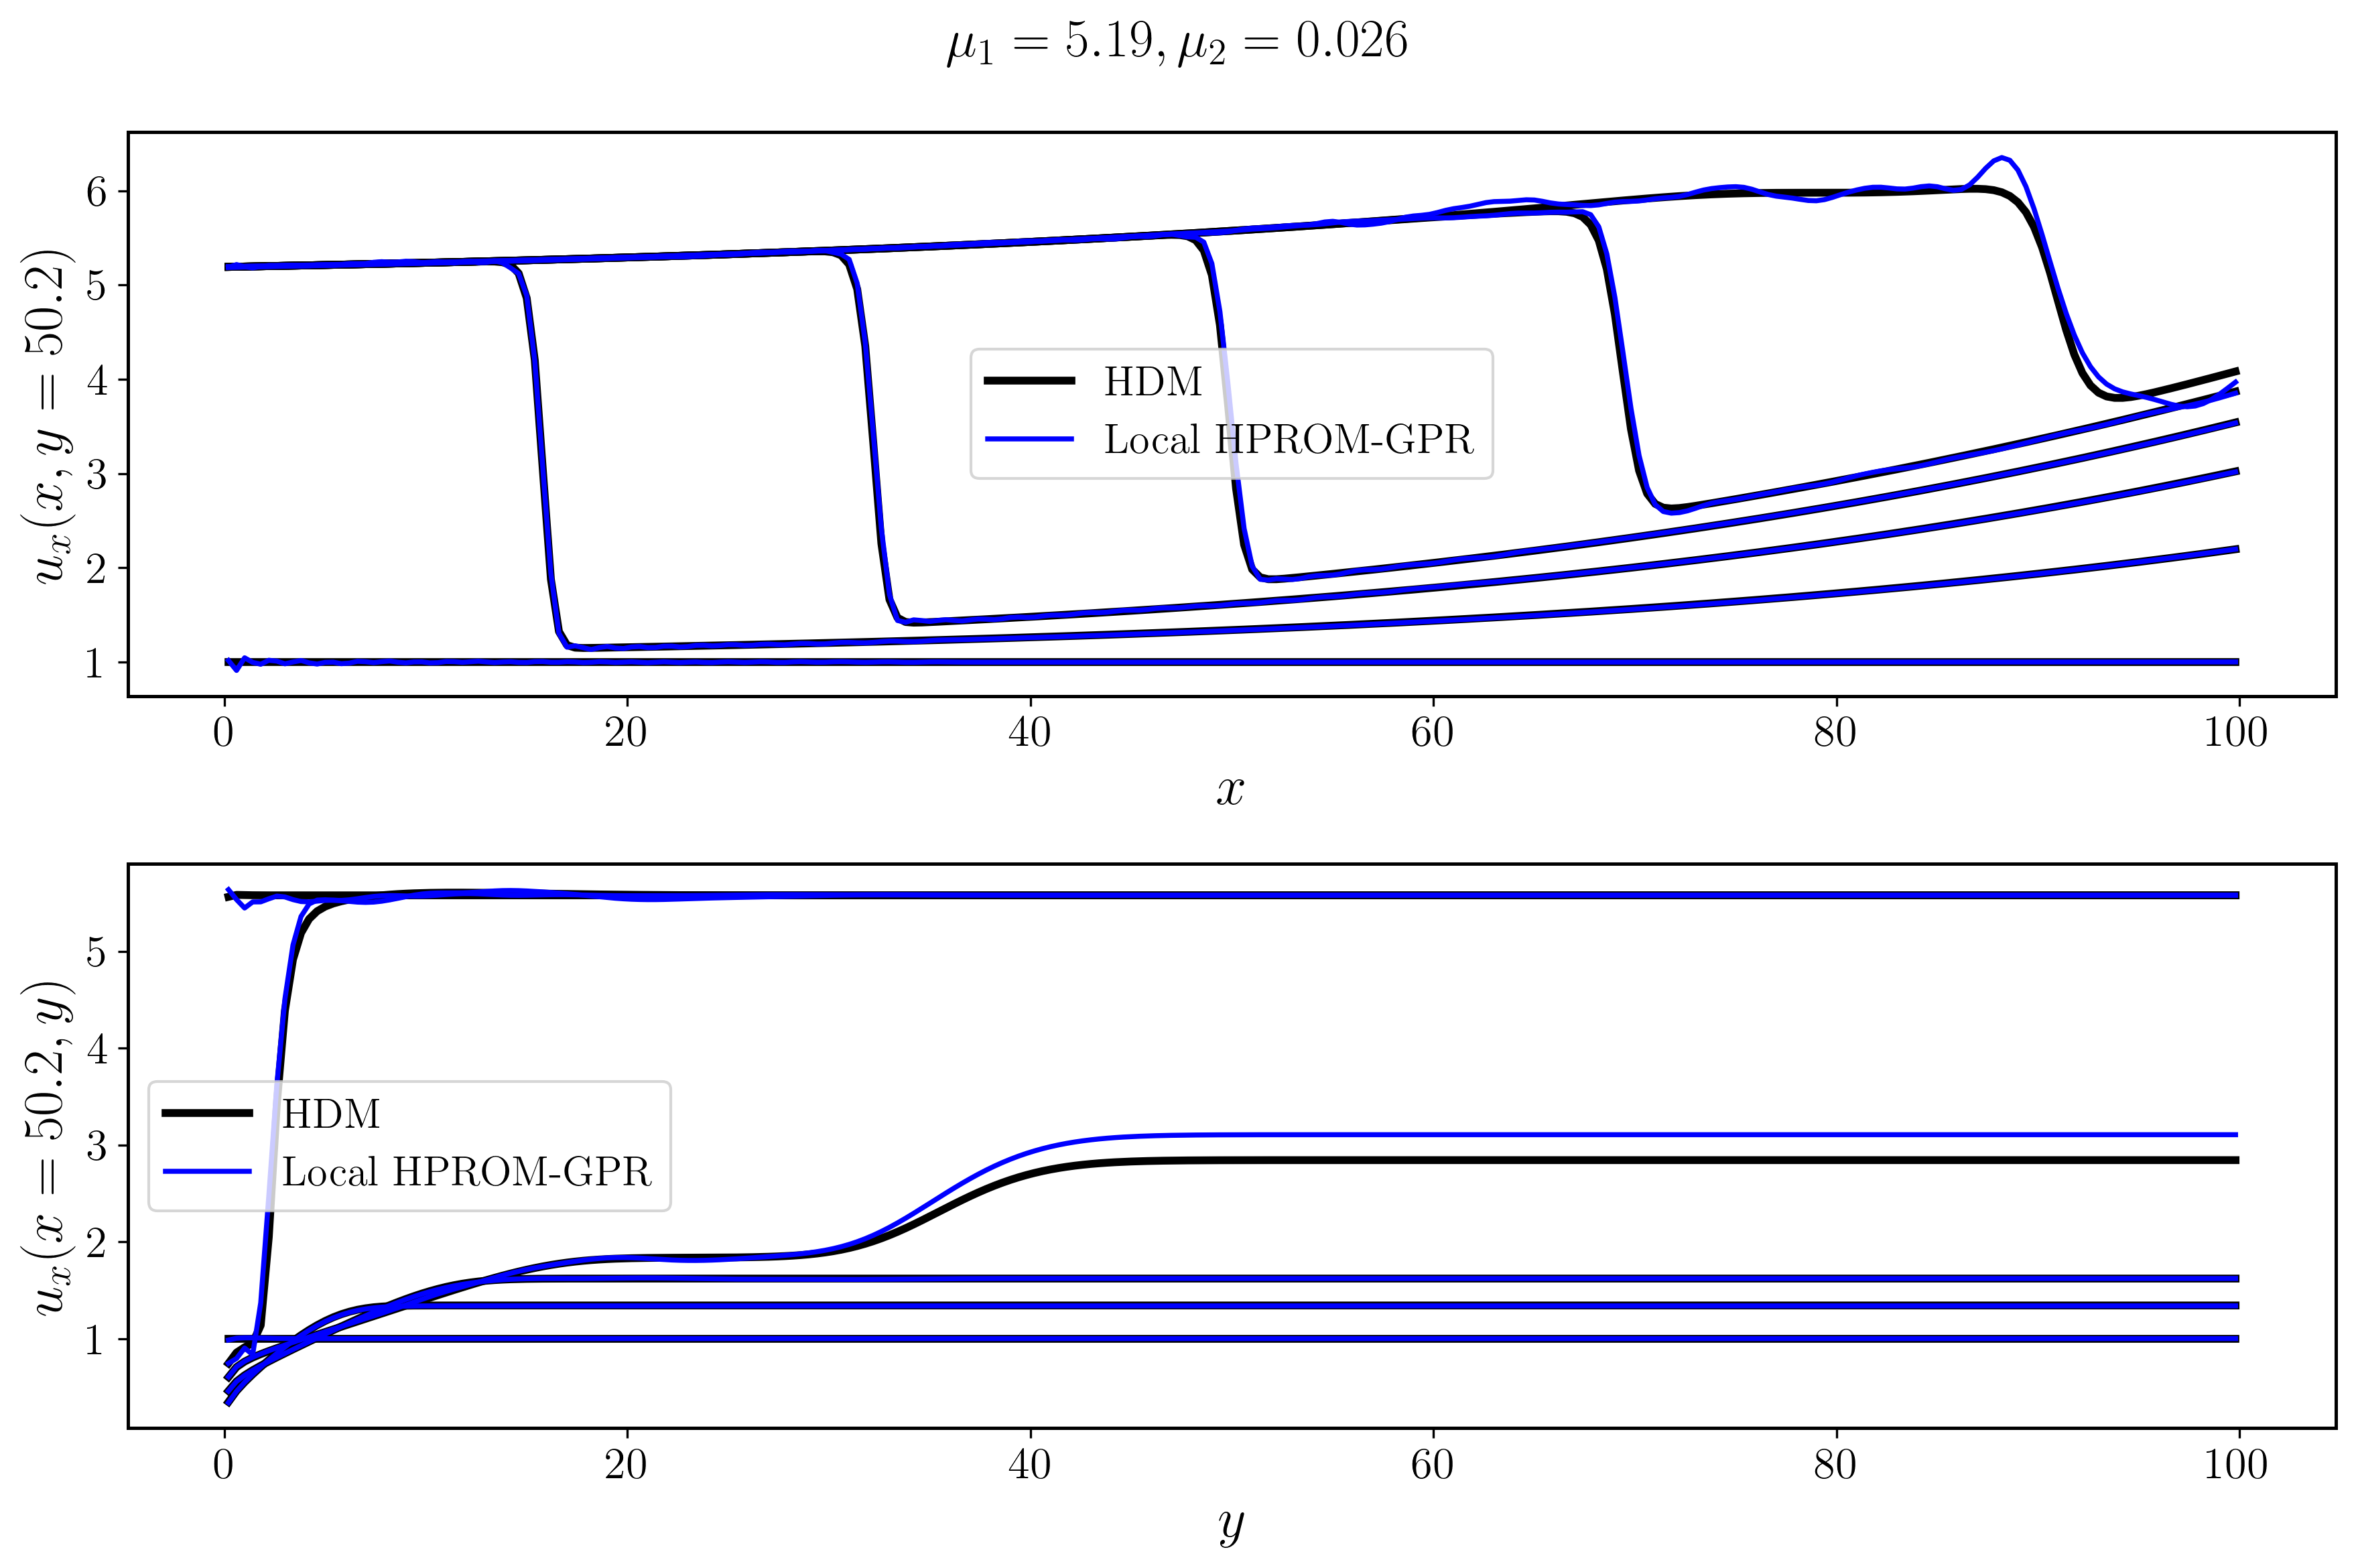
\includegraphics[width=0.82\textwidth,height=0.70\textheight,keepaspectratio]{Figures/local_hprom_gpr_vs_hdm_mu1_5.19_mu2_0.026.png}
\end{frame}

}

\section{Flow Past a Cylinder Campaign}

\begin{frame}{Flow Past a Cylinder Campaign}
\centering
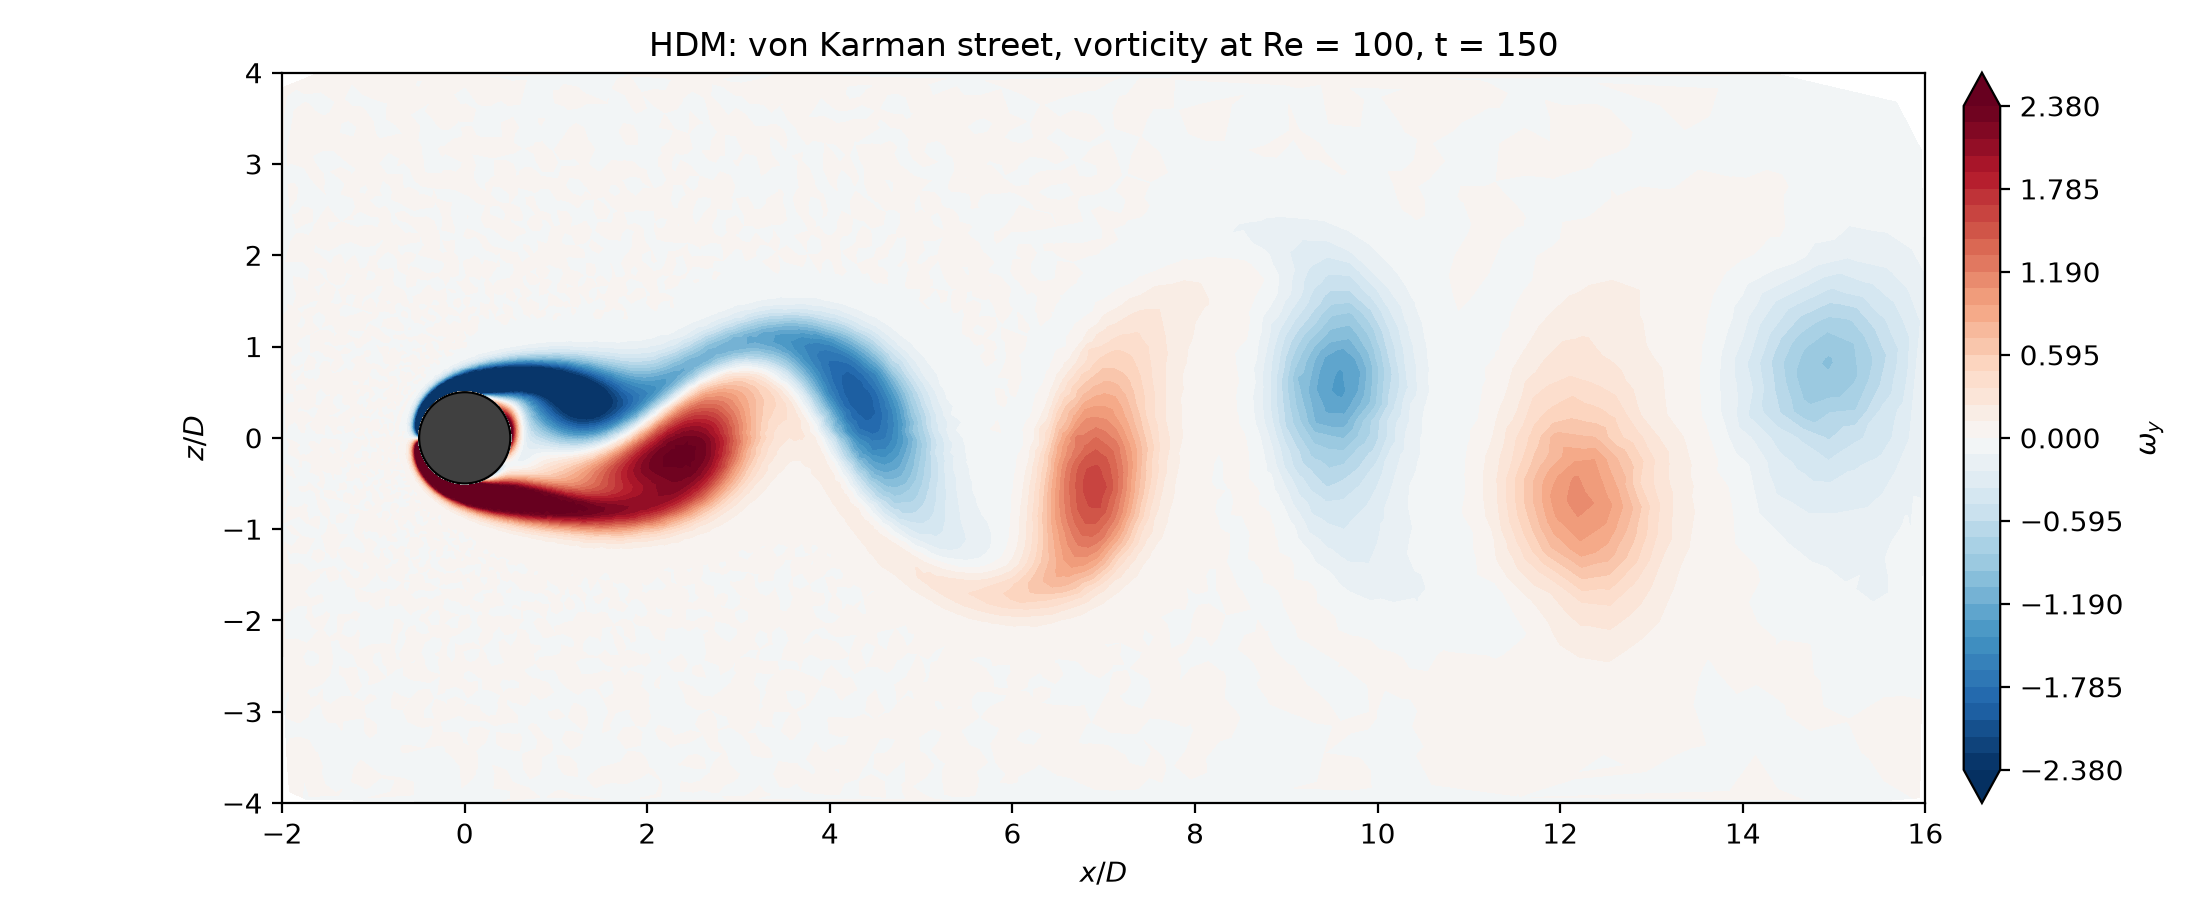
\includegraphics[width=0.86\textwidth]{Figures/cylinder_hdm_vorticity.png}\\[0.18cm]
\normalsize Global and local HPROM validation on an AERO-F CFD model\\[0.10cm]
\small Linear POD bases, quadratic manifolds, and ANN, RBF and GPR manifolds\\[0.10cm]
\small Reproductive regime at $Re=100$, $M_\infty=0.2$: one operating point, no parameter dependence
\end{frame}

\begin{frame}{Cylinder Online Performance and Accuracy ($Re=100$, reproductive)}
\scriptsize
\centering
\resizebox{\textwidth}{!}{%
\begin{tabular}{lrrrrrrr}
\hline
\textbf{Computational model} & $n$ ($N$ for HDM) & $\bar{n}$ & $N_e$ & $\mathbb{W}_{2,C_D}$ (\%) & $\mathbb{W}_{2,C_L}$ (\%) & Wall-clock time (s) & Speedup \\
\hline
HDM & 499\,485 & -- & 284\,700 & -- & -- & 13\,000 & -- \\
\addlinespace[0.35em]
HPROM & 35 & -- & 15\,791 & 0.138 & 0.66 & 8.00 & 1\,625 \\
HQPROM & 10 & -- & 9\,443 & 0.015 & 0.30 & 2.67 & 4\,869 \\
HPROM--ANN & 5 & 30 & 5\,459 & 0.110 & 1.31 & 1.88 & 6\,915 \\
HPROM--RBF & 5 & 30 & 5\,143 & 0.033 & 0.51 & 1.40 & 9\,286 \\
HPROM--GPR & 5 & 30 & 4\,911 & 0.036 & 0.37 & 1.33 & 9\,774 \\
\addlinespace[0.35em]
Local HPROM ($N_c=3$) & 14--35 & -- & 12\,019 & 0.015 & 1.09 & 3.48 & 3\,736 \\
Local HQPROM ($N_c=3$) & 7--10 & -- & 8\,645 & 0.231 & 4.69 & 1.83 & 7\,104 \\
Local HPROM--ANN ($N_c=3$) & 3 & 11--32 & 3\,763 & 0.208 & 2.57 & 1.56 & 8\,333 \\
Local HPROM--RBF ($N_c=3$) & 3 & 11--32 & 4\,340 & 0.027 & 0.81 & 0.87 & 14\,943 \\
Local HPROM--GPR ($N_c=3$) & 3 & 11--32 & 3\,395 & 0.103 & 1.59 & 0.71 & 18\,310 \\
\hline
\end{tabular}}
\vspace{0.2em}

{\tiny Speedup is with respect to $t_{\mathrm{HDM}}=13\,000$ s; timings are the median of five serial repetitions on an idle machine, 8 MPI ranks (CV 2--4\%).}

{\tiny $N_e$ is the number of elements in the ECSW reduced mesh ($284\,700$ for the full mesh).}

{\tiny $\mathbb{W}_2$ is the quadratic Wasserstein distance between the value distributions of the two force histories over the limit cycle, normalized by $\bar{C}_D$ and by $C_L'$ respectively. It measures orbit amplitude and shape and is invariant to phase; frequency accuracy is reported separately in the appendix.}
\end{frame}

\begin{frame}{Cylinder Observations}
\small
\begin{itemize}
  \item The speedup increases monotonically with the degree of nonlinear compression,
        and in the same order globally and locally:
        HPROM $\to$ HQPROM $\to$ ANN $\to$ RBF $\to$ GPR gives
        $1\,625\to4\,869\to6\,915\to9\,286\to9\,774\times$, and
        $3\,736\to7\,104\to8\,333\to14\,943\to18\,310\times$.
  \item Clustering pays in every family: each local model is faster than its global
        counterpart, by $1.21\times$ to $2.30\times$, consistent with the Burgers
        campaign.
\end{itemize}

\vspace{0.3em}
{\footnotesize Preliminary results: no parameter. One operating point, so the models
are tested where they were trained.}

\vspace{0.15em}
{\footnotesize \textbf{Open question:} parameterize this case in $Re$ -- and then, for
the paper, Burgers, the cylinder, or both?}
\end{frame}

\section{Hypersonic Vehicle Campaign}

\begin{frame}{Hypersonic Vehicle Campaign}
\centering
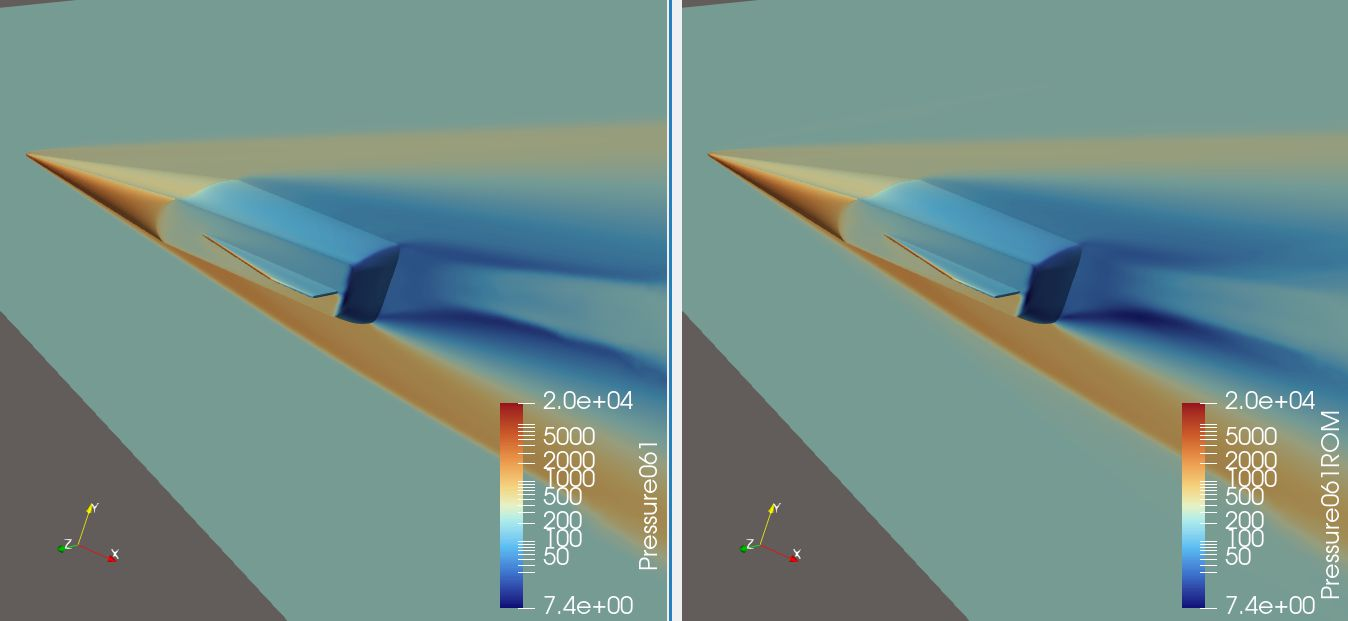
\includegraphics[width=\textwidth,height=0.59\textheight,keepaspectratio]{Figures/img38.jpg}\\[0.25cm]
\Large Global and local HPROM validation\\[0.16cm]
\normalsize Linear POD bases and RBF manifolds
\end{frame}

\begin{frame}{Training and Validation Space}
\centering
\small
363 HDM training cases; 100 independent HDM validation cases; four local clusters with 20\% overlap; ECSW tolerance $10^{-3}$.

\vspace{0.35cm}
\includegraphics[width=0.97\textwidth,height=0.64\textheight,keepaspectratio]{training_validation_space.png}
\end{frame}


\begin{frame}{HGV2 Online Performance and Validation Accuracy}
\scriptsize
\centering
\resizebox{\textwidth}{!}{%
\begin{tabular}{lrrrrrrr}
\hline
\textbf{Computational model} & $n$ ($N$ for HDM) & $\bar{n}$ & $C_D$ (\%) & $C_L$ (\%) & $C_M$ (\%) & Online time (s) & Speedup \\
\hline
HDM & 5\,674\,883 & -- & -- & -- & -- & \textit{pending} & -- \\
\addlinespace[0.35em]
HPROM & 362 & -- & 0.975 & 0.554 & 6.620 & 24.03 & -- \\
HPROM--RBF & 8 & 354 & 1.388 & 1.335 & 7.004 & 1.15 & 21.0 \\
\addlinespace[0.35em]
Local HPROM ($N_c=4$) & 95--168 & -- & 1.101 & 0.444 & 6.242 & 6.80 & 3.5 \\
Local HPROM--RBF ($N_c=4$) & 8 & 117--140 & 1.978 & 2.183 & 7.117 & 0.62 & 38.9 \\
\hline
\end{tabular}}
\vspace{0.2em}

{\tiny Coefficient errors are global relative $L^2$ values over 100 independent validation cases.}

{\tiny Speedup is computed with respect to the HPROM online time, so HPROM itself carries no entry. The HDM runtime is pending.}

{\tiny Timings are means over 10 validation cases, measured on Sherlock using one node, 24 MPI ranks, and 24 cores.}

{\tiny For the HDM, $N$ is the number of mesh nodes. For HPROM, $n$ is the full POD rank. For HPROM--RBF, $n$ and $\bar{n}$ are the primary and secondary dimensions; local $\bar{n}$ is the range across the four cluster bases.}
\end{frame}

\begin{frame}{HGV2 Conclusions}
\small
\begin{itemize}
  \item All four models are equally usable: $C_D$ and $C_L$ within $1$--$2\%$, $C_M$
        within $6.2$--$7.1\%$. The linear models are the most accurate, the RBF models
        the fastest.
  \item RBF closure supplies the compression on its own: $n=8$ against a full POD rank
        of $362$. Clustering does not reduce $n$ further, but it doubles the speed.
  \item The practical gain is where each model runs: the HDM, at $N=5.7$M, needs
        Sherlock, while every ROM here answers in under a second on a single node.
\end{itemize}

\vspace{0.3em}
{\footnotesize HQPROM and Local HQPROM are not included in this campaign.}
\end{frame}

\appendix

\section{Appendix}

\begin{frame}{Appendix}
\centering
\Large Supplementary results and implementation details
\end{frame}

\section{Theory}
\BurgersTheoryFrames

\section{Burgers Setup and Solution Comparisons}

\begin{frame}{Appendix: Burgers Paper Campaign Setup}
\small
\textbf{Two-dimensional parametric inviscid Burgers problem}
\[
\frac{\partial \mathbf U}{\partial t}
+\frac{\partial \mathbf F(\mathbf U)}{\partial x}
+\frac{\partial \mathbf G(\mathbf U)}{\partial y}
=\mathbf S(x;\boldsymbol\mu),
\qquad
\mathbf U=
\begin{bmatrix}
u_x\\u_y
\end{bmatrix}.
\]
\[
\mathbf S(x;\boldsymbol\mu)=
\begin{bmatrix}
0.02\exp(\mu_2 x)\\0
\end{bmatrix},
\qquad
u_x(0,y,t;\boldsymbol\mu)=\mu_1.
\]

\vspace{-0.35em}
\centering
\(\mu_1\): inflow value \qquad
\(\mu_2\): exponential source variation \qquad
\(\boldsymbol\mu\in[4.25,5.50]\times[0.015,0.030]\)
\par

\vspace{0.35em}
\textbf{Test points:}
\[
\boldsymbol\mu_1=(4.56,0.019),\quad
\boldsymbol\mu_2=(4.75,0.020),\quad
\boldsymbol\mu_3=(5.19,0.026).
\]

\vspace{-0.25em}
\begin{columns}[T,onlytextwidth]
\begin{column}{0.42\textwidth}
\textbf{HDM:} $\Omega=[0,100]^2$, $250\times250$ finite-volume cells.
\end{column}
\begin{column}{0.58\textwidth}
\textbf{Methods included:}
\begin{tabular}{ll}
Global HPROM & Local HPROM \\
Global HQPROM & Local HQPROM \\
Global HPROM--GPR & Local HPROM--GPR
\end{tabular}
\end{column}
\end{columns}
\end{frame}

\BurgersSolutionFigureFrames

\section{Cylinder}

\begin{frame}{Appendix: Cylinder Governing Equations and Discretization}
\scriptsize
\textbf{Compressible Navier--Stokes}, perfect gas, laminar (no turbulence closure).
\[
\frac{\partial \mathbf{U}}{\partial t}+\nabla\!\cdot\!\mathbf{F}(\mathbf{U})
=\nabla\!\cdot\!\mathbf{F}_v(\mathbf{U},\nabla\mathbf{U}),
\qquad
\mathbf{U}=[\rho,\ \rho\mathbf{v},\ \rho E]^T \in \mathbb{R}^5 .
\]

\vspace{0.2em}
\begin{columns}[T,onlytextwidth]
\begin{column}{0.49\textwidth}
\textbf{Fluid model}
\begin{tabular}{ll}
$\gamma$              & 1.4 \\
$R$                   & 287.1 J/(kg\,K) \\
viscosity             & constant, $\mu=10^{-2}$ \\
turbulence            & none (laminar) \\
$L_{\mathrm{ref}}$    & 1.0 (cylinder diameter)
\end{tabular}

\vspace{0.5em}
\textbf{Boundary conditions}
\begin{tabular}{ll}
inlet      & external, $M_\infty=0.2$ \\
           & $\alpha=\beta=0$ \\
           & $\rho_\infty=1.0$, $p_\infty=17.857$ \\
wall       & adiabatic, full integration \\
far field  & Steger--Warming
\end{tabular}
\end{column}
\begin{column}{0.49\textwidth}
\textbf{Spatial discretization}
\begin{tabular}{ll}
operator        & finite volume \\
convective flux & Roe \\
reconstruction  & linear, $\beta=1/3$ \\
limiter         & \textbf{none} \\
dissipation     & second order \\
gradients       & least squares
\end{tabular}

\vspace{0.5em}
\textbf{Time integration}
\begin{tabular}{ll}
scheme            & implicit, RK2 \\
$\Delta t$        & 0.1, $t\in[0,150]$ \\
Jacobian          & exact matrix-vector \\
Newton            & 10 its, $\varepsilon=10^{-4}$ \\
linear solver     & GMRES(100), $\varepsilon=10^{-4}$ \\
preconditioner    & RAS, fill 1
\end{tabular}
\end{column}
\end{columns}

\vspace{0.4em}
{\tiny No limiter is used because the flow is smooth and subsonic at $M_\infty=0.2$; the
$\beta=1/3$ linear reconstruction gives the scheme its second-order character. The
domain is $[-20,20]^2$ in units of the diameter, discretized with 98\,140 nodes and
284\,700 elements, for $N=499\,485$ degrees of freedom; it is run as a one-cell-thick
extrusion with symmetry planes. Snapshots are written every two steps, giving 751 per
run. MPI decomposition into 8 subdomains, 8 ranks.}
\end{frame}

\begin{frame}{Appendix: Cylinder ROM and Hyperreduction Settings}
\scriptsize
\begin{columns}[T,onlytextwidth]
\begin{column}{0.49\textwidth}
\textbf{Basis construction}
\begin{tabular}{ll}
snapshots            & 751 (one operating point) \\
reference state      & startup solution \\
normalization        & on \\
compression          & thin SVD via QR \\
energy criterion     & $1-\varepsilon_S^2 = 0.9999$ \\
resulting $n$        & 35
\end{tabular}

\vspace{0.5em}
\textbf{Clustering (local models)}
\begin{tabular}{ll}
algorithm       & k-means++ \\
$N_c$           & 3 \\
max iterations  & 150 \\
overlap         & 10\% \\
random seed     & 42 (pinned) \\
partition       & 167 / 298 / 289
\end{tabular}
\end{column}
\begin{column}{0.49\textwidth}
\textbf{Projection and hyperreduction}
\begin{tabular}{ll}
projection        & LSPG, Gauss--Newton \\
least squares     & normal equations \\
Jacobian          & frozen \\
hyperreduction    & ECSW \\
node selection    & sampling/weighting, QR \\
tolerance         & $10^{-2}$ \\
scaling/centering & off
\end{tabular}

\vspace{0.5em}
\textbf{Quadratic manifold}
\begin{tabular}{ll}
solver            & Tikhonov \\
regularization    & GCV, global \\
SV sampling frac. & 0.6 \\
$n$               & 10 (global) \\
columns of $\mathbf{H}$ & $n(n+1)/2=55$
\end{tabular}
\end{column}
\end{columns}

\vspace{0.4em}
{\tiny Closure maps. ANN: one hidden layer of 1000 ReLU units, internal standardization,
Adam with plateau-based decay, early stopping on a 10\% validation split, exported as
TorchScript. RBF: grid search over Gaussian, inverse-multiquadric, multiquadric and
linear kernels and 100 values of $\epsilon\in[0.2,20]$, min-max scaling, selected on a
10\% validation split. GPR: Mat\'ern-3/2 with optimized hyperparameters, four restarts,
standardized inputs and outputs. All three are seeded, so the reported errors are
reproducible bit for bit.}
\end{frame}

\begin{frame}{Appendix: Cylinder Accuracy Breakdown}
\scriptsize
\centering
\resizebox{0.98\textwidth}{!}{%
\begin{tabular}{lrrrrr}
\hline
\textbf{Computational model} & $St$ & $St$ error (\%) & $C_L'$ error (\%) & $\bar{C}_D$ error (\%) & $\mathbb{RE}_{2,C_L}$ (\%) \\
\hline
HDM & 0.16557 & -- & -- & -- & -- \\
\addlinespace[0.35em]
HPROM ($n=35$) & 0.16560 & $+0.02$ & $-0.71$ & $+0.14$ & 1.74 \\
HPROM ($n=10$) & 0.16586 & $+0.17$ & $-10.68$ & $+0.72$ & 14.98 \\
HQPROM & 0.16559 & $+0.01$ & $+0.09$ & $+0.02$ & 19.07 \\
HPROM--ANN & 0.16516 & $-0.25$ & $-1.39$ & $-0.11$ & 35.78 \\
HPROM--RBF & 0.16520 & $-0.23$ & $-0.27$ & $-0.03$ & 18.99 \\
HPROM--GPR & 0.16545 & $-0.08$ & $-0.22$ & $+0.04$ & 5.64 \\
\addlinespace[0.35em]
Local HPROM ($N_c=3$) & 0.16530 & $-0.16$ & $-0.95$ & $-0.01$ & 5.06 \\
Local HQPROM ($N_c=3$) & 0.16385 & $-1.04$ & $-4.38$ & $+0.23$ & 69.41 \\
Local HPROM--ANN ($N_c=3$) & 0.16470 & $-0.53$ & $-2.66$ & $-0.21$ & 53.67 \\
Local HPROM--RBF ($N_c=3$) & 0.16524 & $-0.20$ & $-0.36$ & $-0.03$ & 9.96 \\
Local HPROM--GPR ($N_c=3$) & 0.16499 & $-0.35$ & $-1.67$ & $-0.10$ & 38.22 \\
\hline
\end{tabular}}
\vspace{0.25em}

{\tiny Measured over $t\in[90,150]$, where the limit cycle is stationary (about 10 shedding cycles); $C_L'$ is the rms lift and $\bar{C}_D$ the mean drag. $\mathbb{RE}_{2,C_L}$ is the time-domain relative $L^2$ error of the lift over $t\in[0,150]$, included for reference.}

{\tiny The last column is why the main table reports the spectral norm instead. Every model resolves the shedding frequency to within $1.04\%$ and the mean drag to within $0.72\%$, yet the time-domain lift error spans $1.7$ to $69.4\%$: a $1\%$ frequency error integrates into tens of percent over the 25 shedding cycles of the window. HQPROM is the clearest case -- $+0.01\%$ in $St$, $+0.09\%$ in $C_L'$ and $+0.02\%$ in $\bar{C}_D$, the most accurate of the set at $n=10$, yet $19.07\%$ in time-domain lift. The $n=10$ linear HPROM is the converse: mid-table on $\mathbb{RE}_{2,C_L}$ while carrying a genuine $10.68\%$ amplitude error.}
\end{frame}

\section{HGV2}

\begin{frame}{Appendix: HGV2 ROM Configurations}
\centering
\small
\renewcommand{\arraystretch}{1.15}
\begin{tabular}{lccc}
\hline
\textbf{Model} & \textbf{Reduction} & \textbf{Closure} & $N_c$ \\
\hline
HPROM & one POD basis & -- & 1 \\
HPROM--RBF & $n=8$ primary coordinates & one RBF map & 1 \\
\addlinespace[0.35em]
Local HPROM & one POD basis per cluster & -- & 4 \\
Local HPROM--RBF & $n=8$ primary coordinates & one RBF map per cluster & 4 \\
\hline
\end{tabular}

\vspace{0.5em}
{\small Every POD basis and RBF map is trained from the same 363 HDM parameter cases.
Each online state is assigned to its nearest cluster. ECSW is an independent offline
construction step.}
\end{frame}


\begin{frame}{Appendix: ECSW Training Data}
\centering
\scriptsize
For \texttt{DataType = Jacobian}, each selected parameter solution assigned to cluster $k$ supplies
$m_k^2$ candidate ECSW rows, where
$m_k=\min\!\left(r_k,\ \texttt{MaxNumResidualComponents}\right)$ and
\texttt{MaxNumResidualComponents} $=30$. With row stride $s$, CM reads every $s$-th row of its \texttt{training\_rows} sequence.

\vspace{0.08cm}
\renewcommand{\arraystretch}{1.10}
\setlength{\tabcolsep}{3pt}
\resizebox{0.98\textwidth}{!}{%
\begin{tabular}{lcccc}
\toprule
\textbf{Model} & \textbf{ECSW cases} & \textbf{Row stride} & $m_k$ & \textbf{Rows read by CM} \\
\midrule
Global linear HPROM & 30 & 1 & $\min(362,30)=30$ & $30\times30^2=27{,}000$ \\
Local linear HPROM, $N_c=4$ & 30 & 1 & $\min(r_k,30)=30$ & $30\times30^2=27{,}000$ \\
Global HPROM--RBF, $n=8$ (ablation) & 30 & 1 & $\min(8,30)=8$ & $30\times8^2=1{,}920$ \\
Global HPROM--RBF, $n=8$ (final) & 363 & 4 & $\min(8,30)=8$ & $363\times8^2/4=5{,}808$ \\
Local HPROM--RBF, $N_c=4$, $n=8$ & 30 & 1 & $\min(8,30)=8$ & $30\times8^2=1{,}920$ \\
\bottomrule
\end{tabular}
}

\vspace{0.08cm}
\begin{block}{Interpretation}
\tiny An ECSW snapshot is a Jacobian-training row, not a physical-time state. The RBF primary dimension $n=8$---not $\bar n$---sets the $8\times8$ count. A row stride of 4 reads rows $0,4,8,\ldots$ within every selected parameter case; it does not subsample the 363 parameter cases and does not refer to online Newton iterations.
\end{block}
\end{frame}

\begin{frame}{Appendix: HGV2 Reduced-Mesh Construction}
\centering
\scriptsize
\renewcommand{\arraystretch}{1.17}
\setlength{\tabcolsep}{2pt}
\begin{tabular}{lrrrrrrr}
\toprule
Model & L0 & L1 & L2 & L3 & Nodes & Elems. & $N_{\neg L2}$ \\
\midrule
Global linear HPROM & 5,089 & 36,971 & 166,878 & 60,623 & 269,561 & 563,301 & 92,683 \\
Local linear HPROM, 4 clusters & 3,484 & 28,145 & 169,798 & 47,183 & 248,610 & 470,649 & 78,812 \\
Global HPROM--RBF, $n=8$ & 1,715 & 15,809 & 173,072 & 28,648 & 219,244 & 350,921 & 46,172 \\
Local HPROM--RBF, 4 clusters, $n=8$ & 1,113 & 10,516 & 175,813 & 20,602 & 208,044 & 298,219 & 32,231 \\
\bottomrule
\end{tabular}

\vspace{0.32cm}
\begin{columns}[T,onlytextwidth]
\begin{column}{0.50\textwidth}
\textbf{L0}: selected ECSW sample nodes.\\
\textbf{L1}: nodes added by edge connectivity for linear reconstruction.
\end{column}
\begin{column}{0.50\textwidth}
\textbf{L2}: lift-surface nodes used only for $C_L$, $C_D$, and $C_M$ postprocessing.\\
\textbf{L3}: nodes added by element connectivity for state reconstruction.
\end{column}
\end{columns}

\vspace{0.18cm}
\footnotesize $N_{\neg L2}$ excludes the postprocessing-only lift-surface nodes.
\end{frame}

\begin{frame}{HGV2 Validation Error Comparison}
\centering
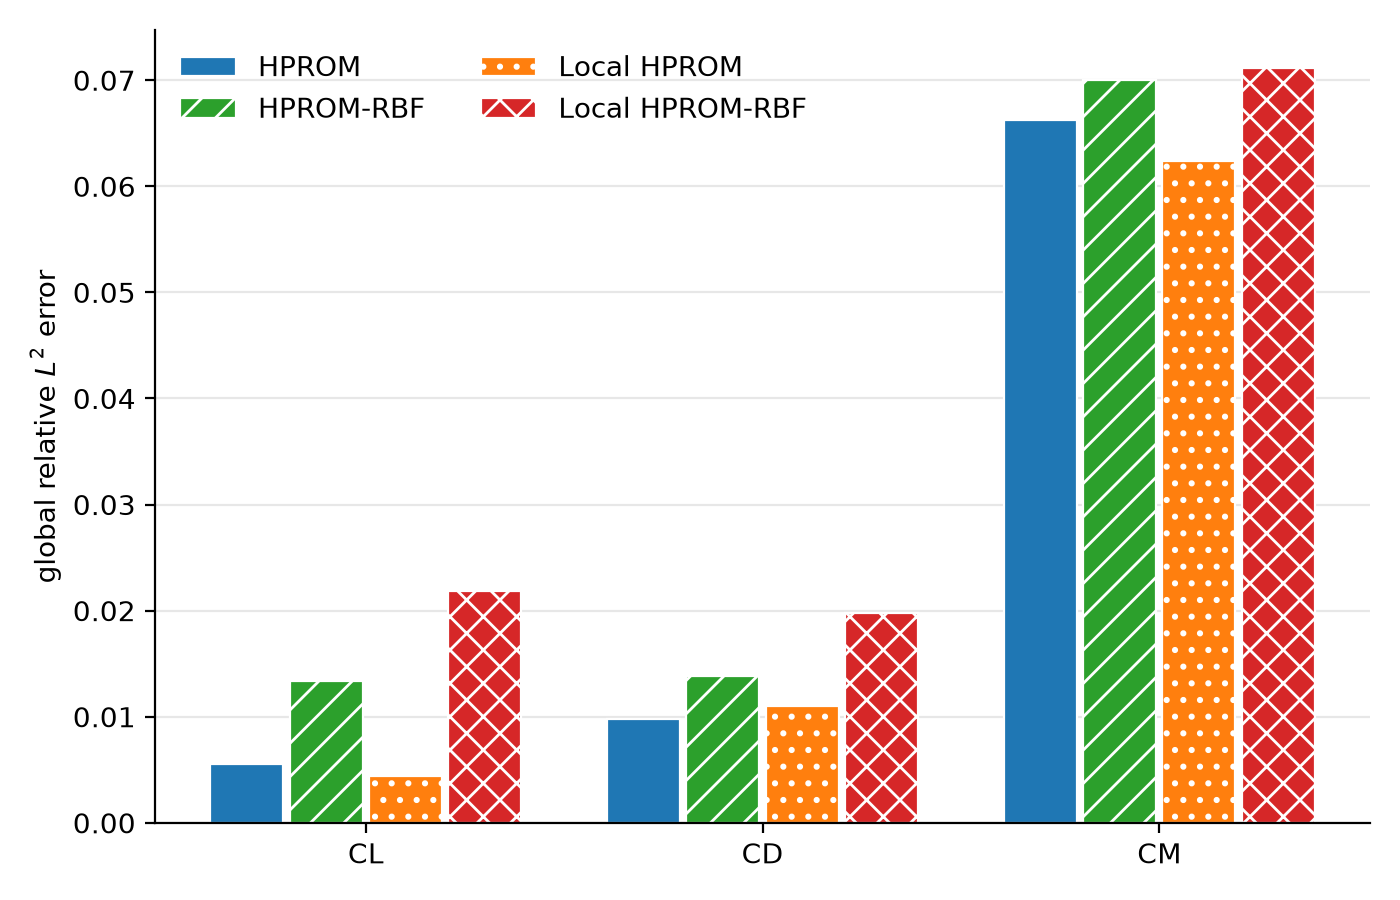
\includegraphics[width=0.91\textwidth,height=0.74\textheight,keepaspectratio]{overall_relative_errors.png}
\end{frame}

\begin{frame}{HGV2 ECSW Offline Cost}
\centering
\scriptsize
\renewcommand{\arraystretch}{1.20}
\resizebox{0.86\textwidth}{!}{%
\begin{tabular}{lrrr}
\hline
\textbf{Computational model} & \textbf{Training rows} & \textbf{Sample nodes} & \textbf{ECSW (h)} \\
\hline
HPROM & 27\,000 & 5\,089 & 30.04 \\
HPROM--RBF & 5\,808 & 1\,715 & 0.43 \\
\addlinespace[0.35em]
Local HPROM ($N_c=4$) & 27\,000 & 3\,484 & 9.95 \\
Local HPROM--RBF ($N_c=4$) & 1\,920 & 1\,113 & 0.38 \\
\hline
\end{tabular}}
\vspace{0.3em}

{\tiny ECSW was run on Sherlock using 20 nodes, 480 MPI ranks, and 480 cores. Times are maximum-rank wall times.}

{\tiny Sample nodes is the size of the reduced mesh. How the training rows are assembled is detailed in the appendix.}
\end{frame}

\begin{frame}{HGV2 Three-Dimensional $C_L$ Error Field}
\centering
\small Each marker is one velocity--altitude pair. Its vertical coordinate is the relative $L^2$ $C_L$ error over the four sampled angles of attack.

\vspace{0.08cm}
\includegraphics[width=0.92\textwidth,height=0.72\textheight,keepaspectratio]{relative_error_3d_CL.png}
\end{frame}

\begin{frame}{HGV2 Two-Dimensional $C_L$ Error Projections}
\centering
\small The front and side projections of the pairwise error field: velocity versus error on the left, altitude versus error on the right.

\vspace{0.08cm}
\includegraphics[width=0.96\textwidth,height=0.72\textheight,keepaspectratio]{relative_error_projections_CL.png}
\end{frame}

\begin{frame}{HGV2 Three-Dimensional $C_D$ Error Field}
\centering
\small Each marker is one velocity--altitude pair. Its vertical coordinate is the relative $L^2$ $C_D$ error over the four sampled angles of attack.

\vspace{0.08cm}
\includegraphics[width=0.92\textwidth,height=0.72\textheight,keepaspectratio]{relative_error_3d_CD.png}
\end{frame}

\begin{frame}{HGV2 Two-Dimensional $C_D$ Error Projections}
\centering
\small The front and side projections of the pairwise error field: velocity versus error on the left, altitude versus error on the right.

\vspace{0.08cm}
\includegraphics[width=0.96\textwidth,height=0.72\textheight,keepaspectratio]{relative_error_projections_CD.png}
\end{frame}

\begin{frame}{HGV2 Three-Dimensional $C_M$ Error Field}
\centering
\small Each marker is one velocity--altitude pair. Its vertical coordinate is the relative $L^2$ $C_M$ error over the four sampled angles of attack.

\vspace{0.08cm}
\includegraphics[width=0.92\textwidth,height=0.72\textheight,keepaspectratio]{relative_error_3d_CM.png}
\end{frame}

\begin{frame}{HGV2 Two-Dimensional $C_M$ Error Projections}
\centering
\small The front and side projections of the pairwise error field: velocity versus error on the left, altitude versus error on the right.

\vspace{0.08cm}
\includegraphics[width=0.96\textwidth,height=0.72\textheight,keepaspectratio]{relative_error_projections_CM.png}
\end{frame}

\begin{frame}{HGV2 Representative Median Pair: $C_L$}
\centering
\small $v=3.495$ km/s, altitude $=59.6$ km. This is the median local-RBF pair after ranking the 25 pairs by the combined $C_L$, $C_D$, and $C_M$ relative-error norm.
\par\vspace{0.06cm}
\includegraphics[width=0.92\textwidth,height=0.70\textheight,keepaspectratio]{coeff_CL_v3495_alt59600.png}
\end{frame}

\begin{frame}{HGV2 Representative Median Pair: $C_D$}
\centering
\small $v=3.495$ km/s, altitude $=59.6$ km. This is the median local-RBF pair after ranking the 25 pairs by the combined $C_L$, $C_D$, and $C_M$ relative-error norm.
\par\vspace{0.06cm}
\includegraphics[width=0.92\textwidth,height=0.70\textheight,keepaspectratio]{coeff_CD_v3495_alt59600.png}
\end{frame}

\begin{frame}{HGV2 Representative Median Pair: $C_M$}
\centering
\small $v=3.495$ km/s, altitude $=59.6$ km. This is the median local-RBF pair after ranking the 25 pairs by the combined $C_L$, $C_D$, and $C_M$ relative-error norm.
\par\vspace{0.06cm}
\includegraphics[width=0.92\textwidth,height=0.70\textheight,keepaspectratio]{coeff_CM_v3495_alt59600.png}
\end{frame}

\begin{frame}{HGV2 Representative Challenging Pair: $C_L$}
\centering
\small $v=3.240$ km/s, altitude $=40.2$ km. This pair has the largest combined local-RBF error across $C_L$, $C_D$, and $C_M$.
\par\vspace{0.06cm}
\includegraphics[width=0.92\textwidth,height=0.70\textheight,keepaspectratio]{coeff_CL_v3240_alt40200.png}
\end{frame}

\begin{frame}{HGV2 Representative Challenging Pair: $C_D$}
\centering
\small $v=3.240$ km/s, altitude $=40.2$ km. This pair has the largest combined local-RBF error across $C_L$, $C_D$, and $C_M$.
\par\vspace{0.06cm}
\includegraphics[width=0.92\textwidth,height=0.70\textheight,keepaspectratio]{coeff_CD_v3240_alt40200.png}
\end{frame}

\begin{frame}{HGV2 Representative Challenging Pair: $C_M$}
\centering
\small $v=3.240$ km/s, altitude $=40.2$ km. This pair has the largest combined local-RBF error across $C_L$, $C_D$, and $C_M$.
\par\vspace{0.06cm}
\includegraphics[width=0.92\textwidth,height=0.70\textheight,keepaspectratio]{coeff_CM_v3240_alt40200.png}
\end{frame}


\end{document}
